\documentclass[12pt]{extreport}
\usepackage[utf8]{vietnam}
\usepackage[left=3.50cm, right=2.00cm, top=1.27cm, bottom=1.27cm]{geometry}
\usepackage{fancybox,graphicx}
\usepackage{mathrsfs} 
\usepackage{amsfonts}
\usepackage{longtable,array}
\usepackage{multirow}
\newlength\mylength
\newcolumntype{C}[1]{>{\centering\arraybackslash}p{#1}}
\usepackage[intlimits]{amsmath}
\usepackage{array}
\usepackage[unicode]{hyperref}
\usepackage{algorithm}
\usepackage{algorithmicx}
\makeatletter
\renewcommand{\ALG@name}{Thuật toán}
\makeatother
\usepackage{algpseudocode}
\usepackage{amsxtra,amssymb,latexsym,amscd,amsthm}
\usepackage{enumitem}
\usepackage{tikz}
\usetikzlibrary{shapes.geometric}
\usetikzlibrary{positioning,automata}
\usepackage{scrextend}
\usepackage{longfbox}
\usepackage{xcolor}
\usepackage{listings}
\usepackage{ragged2e}
\usepackage{caption}
\usepackage{subcaption}
\usepackage{adjustbox}
\usepackage{diagbox}

\definecolor{mGreen}{rgb}{0,0.6,0}
\definecolor{mGray}{rgb}{0.5,0.5,0.5}
\definecolor{mPurple}{rgb}{0.58,0,0.82}
\definecolor{backgroundColour}{rgb}{0.95,0.95,0.92}

\lstdefinestyle{PythonStyle}{
	backgroundcolor=\color{backgroundColour},   
	commentstyle=\color{mGreen},
	keywordstyle=\color{magenta},
	numberstyle=\tiny\color{mGray},
	stringstyle=\color{mPurple},
	basicstyle=\footnotesize,
	breakatwhitespace=false,         
	breaklines=true,                 
	captionpos=b,                    
	keepspaces=true,                 
	numbers=left,                    
	numbersep=5pt,                  
	showspaces=false,                
	showstringspaces=false,
	showtabs=false,                  
	tabsize=2,
	language=Python
}

\bibliographystyle{unsrt}


\begin{document}

\thispagestyle{empty}
\thisfancypage{
    \setlength{\fboxsep}{0pt}
    \fbox}{}

\begin{center}
    {\fontsize{13pt}{1}\selectfont\textbf{TRƯỜNG ĐẠI HỌC BÁCH KHOA HÀ NỘI}}
    \\
    {\fontsize{13pt}{1}\selectfont\textbf{VIỆN CÔNG NGHỆ THÔNG TIN VÀ TRUYỀN THÔNG}}
    \\
    \textbf{--------------------  o0o  ---------------------}\\[1cm]
    
\includegraphics[scale=0.5]{bk-rgb.jpg} \\[1.2cm]
    \textbf{\large{ĐỒ ÁN TỐT NGHIỆP}}\\[1cm]
    \textbf{\large{Sử dụng mô hình StarGAN v2 để \\ đổi chế độ màu ảnh nội soi y tế}}\\[1cm]
    Trần Minh Hiếu - 20160075 \\
    Lớp Chương trình Tài Năng - Công nghệ Thông tin
\end{center}

\vspace{1.5cm}
\begin{center}
    \begin{tabular}{l l c}
        \textbf{Giảng viên hướng dẫn:} & TS. Đinh Viết Sang                  & \hrulefill                                \\
        \textbf{Bộ môn:}               & Khoa học Máy tính                   & \fontsize{8pt}{1}\selectfont{Chữ kí GVHD} \\
        \textbf{Viện:}                 & Công nghệ Thông tin và Truyền thông &                                           \\
    \end{tabular}
\end{center}

\vspace{1.0cm}
\begin{center}
    \textbf{{Hà Nội, tháng 5/2021}}\\
\end{center}

\newpage

\begin{center}
    \fontsize{8pt}{1}\selectfont{
        \begin{tabular}{c c}
            BỘ GIÁO DỤC \& ĐÀO TẠO                   & \textbf{CỘNG HÒA XÃ HỘI CHỦ NGHĨA VIỆT NAM} \\
            \textbf{TRƯỜNG ĐẠI HỌC BÁCH KHOA HÀ NỘI} & \textbf{Độc lập - Tự do - Hạnh phúc}
        \end{tabular}
    }
\end{center}

\vspace{1.0cm}
\begin{center}
    \large\textbf{NHIỆM VỤ \\
        ĐỒ ÁN TỐT NGHIỆP}
\end{center}

\vspace{0.5cm}
\justify
Họ và tên sinh viên: Trần Minh Hiếu \\
Khóa: K62, Viện: Công nghệ Thông tin và Truyền thông, Lớp: Chương trình Tài Năng

\textit{1. Tên đề tài}

Sử dụng mô hình StarGAN v2 để đổi chế độ màu ảnh nội soi y tế.

\textit{2. Nội dung đề tài}

Ung thư đường tiêu hóa là một trong những nguyên nhân gây tử vong hàng đầu trên thế giới. May mắn thay, sự phát triển của công nghệ nội soi đường tiêu hóa giúp chúng ta có thể sớm nhận biết và điều trị các triệu chứng ung thư, đặc biệt là trong giai đoạn đầu của bệnh lý. Từ những năm 2000, các kĩ thuật tăng cường chất lượng ảnh nội soi bằng phần cứng (hardware-based image-enhanced endoscopy hay IEE) như BLI (Blue Laser Imagining) hay LCI (Linked Color Imagining) bắt đầu trở nên phổ biến, dần thay thế các kĩ thuật nội soi sử dụng đèn trắng nhuộm màu như WLI (White Light Imagining). Tuy nhiên, do những hạn chế về ngân sách và chính sách đầu tư, việc triển khai các dụng cụ nội soi tích hợp các chức năng này còn gặp nhiều khó khăn.

Đồ án này hướng tới việc đào tạo mô hình học sâu (Deep Learning) StarGAN v2 để đổi màu hình ảnh nội soi thuộc chế độ màu sắc cơ bản sang các chế độ màu sắc cao cấp, cũng như tích hợp mô hình này vào hệ thống gắn nhãn ảnh nội soi y tế Polyp-Labeler đang được triển khai trên thực tế. Qua đồ án tốt nghiệp này, em hy vọng có thể giúp các bác sĩ nội soi tiếp cận với những chức năng nội soi tiên tiến mà không bị rào cản về kinh tế ngăn cản.

\textit{3. Cán bộ hướng dẫn}

TS. Đinh Viết Sang, giảng viên bộ môn Khoa học Máy tính, viện Công nghệ Thông tin và Truyền thông, trường Đại học Bách khoa Hà Nội.

\textit{4. Thời gian giao đề tài}

Tháng 2 năm 2021.

\textit{5. Thời gian hoàn thành}

Tháng 6 năm 2021.

\vspace{1cm}
\begin{center}
    \fontsize{10pt}{1}\selectfont{
        \begin{tabular}{c c c}
            \textit{Hà Nội, ngày 5 tháng 5 năm 2021} &                           &                                \\
            \textbf{LÃNH ĐẠO BỘ MÔN}                 & \textbf{CÁN BỘ HƯỚNG DẪN} & \textbf{SINH VIÊN THỰC HIỆN}   \\
                                                     &                           & \textit{(Ký và ghi rõ họ tên)}
        \end{tabular}
    }
\end{center}

\chapter*{Lời cảm ơn}

Em xin chân thành cảm ơn thầy Đinh Viết Sang, giảng viên hướng dẫn bộ môn Đồ án Tốt nghiệp đã hướng dẫn và tài trợ cơ sở hạ tầng để em có thể hoàn thiện được đồ án này.

Em cũng xin gửi lời cảm ơn tới các bác sĩ của Viện nghiên cứu và đào tạo tiêu hoá gan mật IGH đã cung cấp bộ dữ liệu ảnh nội soi gắn nhãn được sử dụng trong đề tài, cũng như vì đã nhiệt tình giúp đỡ trong toàn bộ quá trình thực hiện dự án Polyp-Labeler.

\tableofcontents

\chapter{Tổng quan về bài toán và đặt vấn đề}

Ung thư đường tiêu hóa là một trong những nguyên nhân gây tử vong hàng đầu trên thế giới. Chỉ tính riêng trong năm 2018, đã có hơn 1 triệu bệnh nhân được chẩn đoán ung thư dạ dày trên toàn cầu, với khoảng 783,000 ca tử vong. Ung thư dạ dày là bệnh lý ung thư phổ biến thứ 5 và gây ra tử vong nhiều thứ 3 trên thế giới \cite{https://doi.org/10.3322/caac.21492}. May mắn thay, ung thư đường tiêu hóa có thể được điều trị và chữa khỏi nếu được phát hiện kịp thời. Những tiến bộ trong công nghệ nội soi đóng vai trò quan trọng trong việc phát hiện những biểu hiện bệnh lý giai đoạn đầu, qua đó giúp các bác sĩ có thể kịp thời đưa ra pháp đồ điều trị.

Phương pháp nội soi cơ bản nhất - nội soi sử dụng đèn trắng (White Light Imagining hay WLI) - được đưa vào sử dụng rộng rãi trong việc phát hiện ung thư trực tràng từ cuối những năm 50 của thế kỉ trước \cite{pmid26668791}. Qua thời gian, các bác sĩ nội soi bắt đầu sử dụng đèn nhuộm màu để làm rõ các thương tổn trong đường tiêu hóa và dễ dàng đưa ra chẩn đoán hơn. Phương pháp nhuộm màu lăng kính thủ công được sử dụng phổ biến vào những năm 90 của thế kỉ trước: sau khi nội soi lần một để tìm các điểm quan trọng, lăng kính được nhuộm màu bằng thuốc nhuộm dạng xịt, và bác sĩ tập trung quan sát khối u để đưa ra nhận xét cuối cùng \cite{pmid10613481}.

Tới những năm 2000, phương pháp này bị thay thế bởi các công nghệ đổi màu bằng phần cứng (hardware-based Image-Enhanced Endoscopy, viết tắt là IEE). Các phương pháp IEE tiện lợi hơn phương pháp nhuộm màu lăng kính vì cho phép bác sĩ có thể tăng cường chất lượng ảnh chỉ bằng một thao tác bên ngoài, thay vì phải rút ống để nhuộm màu và nội soi lại lần hai.

Các phương pháp IEE đời đầu bao gồm NBI - Narrow Band Imagining \cite{pmid15578301}, FICE - Flexible spectral Imagining Color Enhancement \cite{TOGASHI2009734} và i-Scan \cite{HOFFMAN201045}. Nhược điểm của các phương pháp thế hệ đầu này là ảnh nội soi bị tối màu và độ phân giải ảnh kém. Trong các thử nghiệm lâm sàng cỡ lớn, các phương pháp này không thật sự nâng cao xác suất chẩn đoán đúng khối u so với phương pháp đèn trắng cổ điển có độ phân giải cao \cite{REX200742} \cite{pmid20628363}.

Vào năm 2013, Fujifilm Corporation cho ra công nghệ Blue Laser Imagining (BLI). BLI có thể cho ra hình ảnh có màu sắc sáng sủa và rõ ràng kể cả ở khoảng cách xa đầu dò, giúp cải thiện độ chính xác trong chẩn đoán ung thư của bác sĩ \cite{pmid24373002}. Fujifilm Corporation tiếp tục phát triển và cho ra công nghệ màu Linked Color Imagining (LCI) vào năm 2014, tích hợp cả khả năng tiền xử lý và hậu xử lý ảnh để tăng cường sự tương phản giữa khối u ác tính và niêm mạc xung quanh \cite{pmid30291440}. Nhờ những chức năng cao cấp này, ảnh nội soi sử dụng BLI và LCI giúp giảm khả năng bỏ sót tổn thương trong quá trình nội soi so với các công nghệ IEE khác.

\begin{figure}[H]
    \centering
    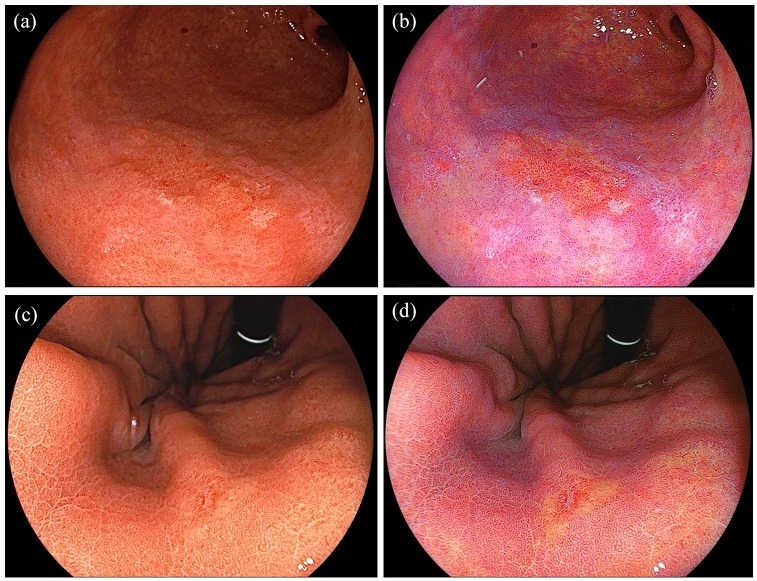
\includegraphics[width=0.7\textwidth]{figure1}
    \caption{So sánh ảnh nội soi ung thư dạ dày giai đoạn đầu. (a) và (c) là ảnh nội soi sử dụng WLI, không làm rõ khối u tuyến trong dạ dày. (b) và (d) là ảnh nội soi sử dụng LCI tại cùng vị trí làm nổi bật rõ khối u tuyến so với niêm mạc xung quanh. Nguồn ảnh: \cite{pmid31700545}.}
    \label{wli-lci}
\end{figure}

Tuy hiệu quả của các công nghệ nội soi mới này đã được chỉ ra trên thực tế, song việc triển khai các thiết bị có tích hợp các công nghệ này còn gặp nhiều khó khăn. Trong một bài báo trên tạp chí Therap Adv Gastroenterol năm 2016, nhóm nghiên cứu chỉ ra rằng phần lớn bác sĩ nội soi tại Nhật Bản vẫn chưa quen sử dụng các thiết bị được trang bị BLI - 3 năm sau khi BLI được phát triển - do các thiết bị này chưa được triển khai rộng rãi tại các cơ sở y tế \cite{pmid26770267}. Hạn chế về chi phí là rào cản lớn ngăn cản các bác sĩ nội soi có thể tiếp cận với các công nghệ mới này, đặc biệt là ở các cơ sở y tế địa phương và vùng sâu vùng xa.

Để khắc phục hạn chế về cơ sở hạ tầng, ta có thể sử dụng phần mềm để tái tạo lại các chức năng nội soi cao cấp này. Trong thời gian gần đây, các giải pháp học máy (Machine Learning) nói chung và học sâu (Deep Learning) nói riêng đang trở nên rất phổ biến - thay vì chỉnh sửa các thông số thuật toán một cách thủ công, lập trình viên có thể cho mô hình trí tuệ nhân tạo tiếp xúc với một lượng lớn dữ liệu, và các thông số của mô hình sẽ được tối ưu tự động (\textit{"học"}) để tối đa mục tiêu của bài toán. Với thiết kế mô hình và chiến lược luyện tập mô hình hợp lý, ta có thể tạo ra những mô hình chất lượng cao.

\textit{\textbf{Trong đồ án tốt nghiệp này, em hướng tới việc sử dụng mô hình học máy StarGAN v2, phát triển bởi các nhà nghiên cứu của Clova AI thuộc tập đoàn NAVER, để thực hiện chức năng đổi màu cho ảnh nội soi giữa 4 chế độ màu tiêu biểu - BLI, FICE, LCI và WLI.}}

Báo cáo đồ án được chia làm 6 chương:
\begin{enumerate}
    \item \textbf{Chương 1 - Tổng quan về bài toán và đặt vấn đề}, giải thích bài toán và ứng dụng của đề tài trong thực tế.
    \item \textbf{Chương 2 - Cơ sở lý thuyết và nghiên cứu liên quan}, đi qua các cơ sở lý thuyết về Machine Learning, Deep Learning, Generative Adversarial Network (GAN) cùng với các nghiên cứu có liên quan tới đề tài, trước khi giải thích lý do lựa chọn mô hình StarGAN v2.
    \item \textbf{Chương 3 - Phương pháp đề xuất}, giải thích kiến trúc mô hình StarGAN v2 và các hàm mục tiêu được sử dụng trong quá trình luyện tập mô hình.
    \item \textbf{Chương 4 - Thử nghiệm và đánh giá}, mô tả môi trường luyện tập mô hình và kết quả đánh giá chất lượng sản phẩm.
    \item \textbf{Chương 5 - Ứng dụng thực tế - áp dụng vào hệ thống Polyp-Labeler}, nói về dự án Polyp-Labeler, hiện đang được sử dụng bởi các bác sĩ của Viện nghiên cứu và đào tạo tiêu hoá gan mật IGH, và quá trình ứng dụng sản phẩm của đề tài vào hệ thống của dự án.
    \item \textbf{Chương 6 - Kết luận và hướng phát triển}.
\end{enumerate}

\chapter{Cơ sở lý thuyết và nghiên cứu liên quan}

\section{Một số khái niệm cơ bản về học máy}

\subsection{Học máy là gì?}

Học máy (Machine Learning) là một lĩnh vực con của trí tuệ nhân tạo, xoay quanh việc thiết kế các thuật toán có khả năng tự cải thiện thông qua việc tiếp xúc với dữ liệu luyện tập, thay vì được cài đặt lời giải cụ thể một cách thủ công. Học máy được áp dụng rộng rãi để giải nhiều bài toán khó, gần như không thể được giải quyết bằng những thuật toán thủ công trong nhiều lĩnh vực như y học, thị giác máy tính, xử lý ngôn ngữ tự nhiên\dots

Các thuật toán học máy tiêu biểu gồm có Decision Tree, Naive Bayes, SVM, K-Means, Neural Network, vân vân... Các thuật toán này có thể được phân chia làm nhiều nhóm, tùy vào mục đích, kiến trúc và lượng dữ liệu cần sử dụng.

\subsection{Phân loại học máy}

Các thuật toán học máy thường được chia làm ba phân loại lớn, tùy theo đặc điểm của dữ liệu mà máy được cung cấp là Supervised Learning, Unsupervised Learning và Reinforcement Learning.

\subsubsection{Học có giám sát (Supervised Learning)}

Các thuật toán học có giám sát hướng tới việc xây dựng một mô hình toán học dựa trên dữ liệu mẫu có sẵn đầu vào và đầu ra kì vọng. Bằng cách tối ưu một hoặc nhiều hàm số mục tiêu, ta xây dựng được ước lượng hàm gần đúng, có khả năng ánh xạ từ đầu vào tới đầu ra trong dữ liệu luyện tập. Với mô hình học máy phù hợp, chiến lược luyện tập hợp lý cùng với đủ dữ liệu, mô hình học máy có thể dự đoán chính xác kết quả đầu ra với đầu vào chưa gặp từ trước.

Các mô hình học có giám sát có thể được phân chia nhỏ hơn thành mô hình phân loại (classification) và mô hình suy biến (regression). Mô hình phân loại có thể phân loại dữ liệu đầu vào theo một số lớp dữ liệu đã biết từ trước, trong khi mô hình suy biến hướng tới việc tính ra giá trị thực trong khoảng bất kì.

Các ứng dụng tiêu biểu của học có giám sát bao gồm việc nhận diện chữ viết tay, nhận diện lệnh giọng nói, dự đoán biến động giá cổ phiếu, vân vân\dots

\subsubsection{Học không giám sát (Unsupervised Learning)}

Các thuật toán học không giám sát nhận vào một tập dữ liệu tự do, không có đầu vào đầu ra kì vọng, và hướng tới việc tìm kiếm những xu hướng tiêu biểu trong dữ liệu.

Ứng dụng quen thuộc nhất của các thuật toán học không giám sát là bài toán phân cụm dữ liệu. Giải thuật phân cụm có nhiệm vụ chia dữ liệu đầu vào thành các cụm con, sao cho các dữ liệu trong cùng một cụm có đặc điểm giống nhau, dữ liệu giữa các cụm khác nhau có đặc điểm khác nhau. Sự "giống nhau" và "khác nhau" này được đo đạc bằng các hàm số mục tiêu như khoảng cách Euler, khoảng cách Mahattan, vân vân\dots

\subsubsection{Học tăng cường (Reinforcement Learning)}

Các thuật toán học tăng cường giải quyết bài toán huấn luyện một tác tử thông minh trong một môi trường định sẵn, để tác tử đó có thể tối đa hóa một giá trị phần thưởng tích lũy qua thời gian. Môi trường học tăng cường thường được mô tả dưới dạng một chuỗi quyết định Markov (Markov Decision Process) với công thức toán học không thể định nghĩa được chính xác. Bằng cách xây dựng một ước lượng gần đúng của chuỗi quyết định, tác tử thông minh có thể dần học được cách hoạt động độc lập hiệu quả trong môi trường.

Xe tự lại và trí tuệ nhân tạo chơi trò chơi là các ứng dụng tiêu biểu của phương pháp học tăng cường.

Trong báo cáo đồ án tốt nghiệp này, ta chủ yếu quan tâm tới các phương pháp học có giám sát. Khả năng tìm ra ước lượng hàm thỏa mãn mục tiêu đặt ra là cơ sở xây dựng nên nhiều thuật toán học máy cao cấp, trong đó có mô hình Generative Adversarial Network (GAN) được sử dụng trong đồ án tốt nghiệp này.

\section{Giới thiệu về mạng Nơ-ron (Neural Network)}

Mạng nơ-ron (Neural Network) là một trong những thuật toán học máy có giám sát phổ biến nhất. Lấy cảm hứng từ cơ chế hoạt động của nơ-ron thần kinh trong cơ thể sinh học, mạng nơ-ron là các đồ thị tính toán cực kì phức tạp và hiệu quả trong việc ước lượng mối tương quan giữa dữ liệu đầu vào và đầu ra.

\subsection{Nơ-ron nhân tạo và mạng kết nối đầy đủ (Fully Connected Neural Network)}

\subsubsection{Định nghĩa}

Trong mạng nơ-ron, một nơ-ron nhận vào một số dữ liệu đầu vào $ x_i $ và cho ra một giá trị đầu ra $ y $. Nơ-ron cũng sử dụng một hàm kích hoạt (activation function) $ f(x) $, thường là phi tuyến tính, để biểu diễn sự "kích hoạt" của nơ-ron với một số trạng thái đầu vào nhất định.

Để thực hiện tính toán với một nơ-ron, ta thực hiện lấy tổng có trọng số của các giá trị đầu vào, và đưa giá trị này qua hàm kích hoạt. Tổng có trọng số này thường được bổ sung thêm một giá trị bias $ \beta $, có thể được biểu diễn như là một giá trị độc lập, hoặc như là hệ số $ w_0 $ của giá trị đầu vào hằng số $ x_0 = 1 $:
$$ y = f(\sum_{i=1}^{n} x_i w_i + \beta) = f(\sum_{i=0}^{n} x_i w_i) $$

\begin{figure}[H]
    \centering
    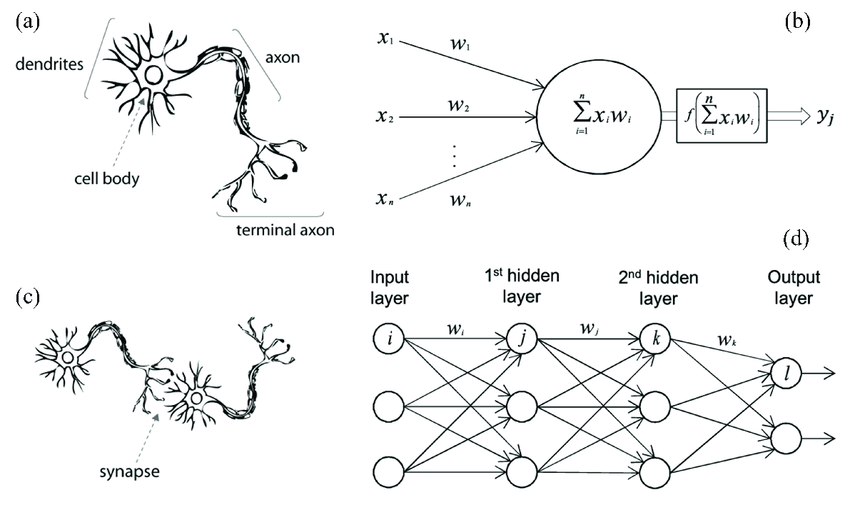
\includegraphics[width=0.8\textwidth]{figure4}
    \caption{So sánh giữa nơ-ron thực tế và nơ-ron trong mạng đầy đủ. Nguồn ảnh: \cite{article}.}
\end{figure}

Mạng nơ-ron được tổ chức thành các lớp, mỗi lớp gồm có nhiều nơ-ron, lấy kết quả đầu ra của lớp trước làm đầu vào cho lớp sau. Lớp đầu tiên của mạng nơ-ron là các thuộc tính của dữ liệu đầu vào, lớp cuối cùng của mạng cho ra kết quả của thuật toán. Giả sử một lớp mạng nhận vào $ n $ giá trị đầu vào và cho ra $ m $ giá trị đầu ra, ta có thể biểu diễn công thức của lớp mạng đó thành:

\begin{center}
    \begin{math}
        Y = \begin{bmatrix}
            y_1 \\
            y_2 \\
            ... \\
            y_m
        \end{bmatrix} = f \left(\begin{bmatrix}
                w_{1,0}, w_{1,1}, \dots, w_{1,n} \\
                w_{2,0}, w_{2,1}, \dots, w_{2,n} \\
                \dots                            \\
                w_{m,0}, w_{m,1}, \dots, w_{m,n} \\
            \end{bmatrix} * \begin{bmatrix}
                1,  \\
                x_1 \\
                x_2 \\
                ... \\
                x_n
            \end{bmatrix} \right) = f(Wx)
    \end{math}
\end{center}

Một lớp mạng nơ-ron dạng này được gọi là lớp mạng nơ-ron đầy đủ (Fully Connected), vì khi biểu diễn trên đồ thị tính toán, mọi phần tử giữa hai lớp mạng sẽ được kết nối với nhau bằng các cạnh có trọng số $ W $. Huấn luyện mạng nơ-ron đầy đủ hướng tới việc tìm ra các giá trị trọng số $ W $ hiệu quả nhất để biểu diễn mối quan hệ giữa đầu vào và đầu ra. Mạng nơ-ron hoạt động hiệu quả nhờ việc tổng hợp tri thức cơ bản học được ở các lớp đầu để cho ra kết quả phức tạp hơn ở các lớp sau. Đây cũng là nguồn gốc của tên gọi Học sâu (Deep Learning) - các mạng nơ-ron thường có rất, rất nhiều lớp - rất "sâu".

\begin{figure}[H]
    \centering
    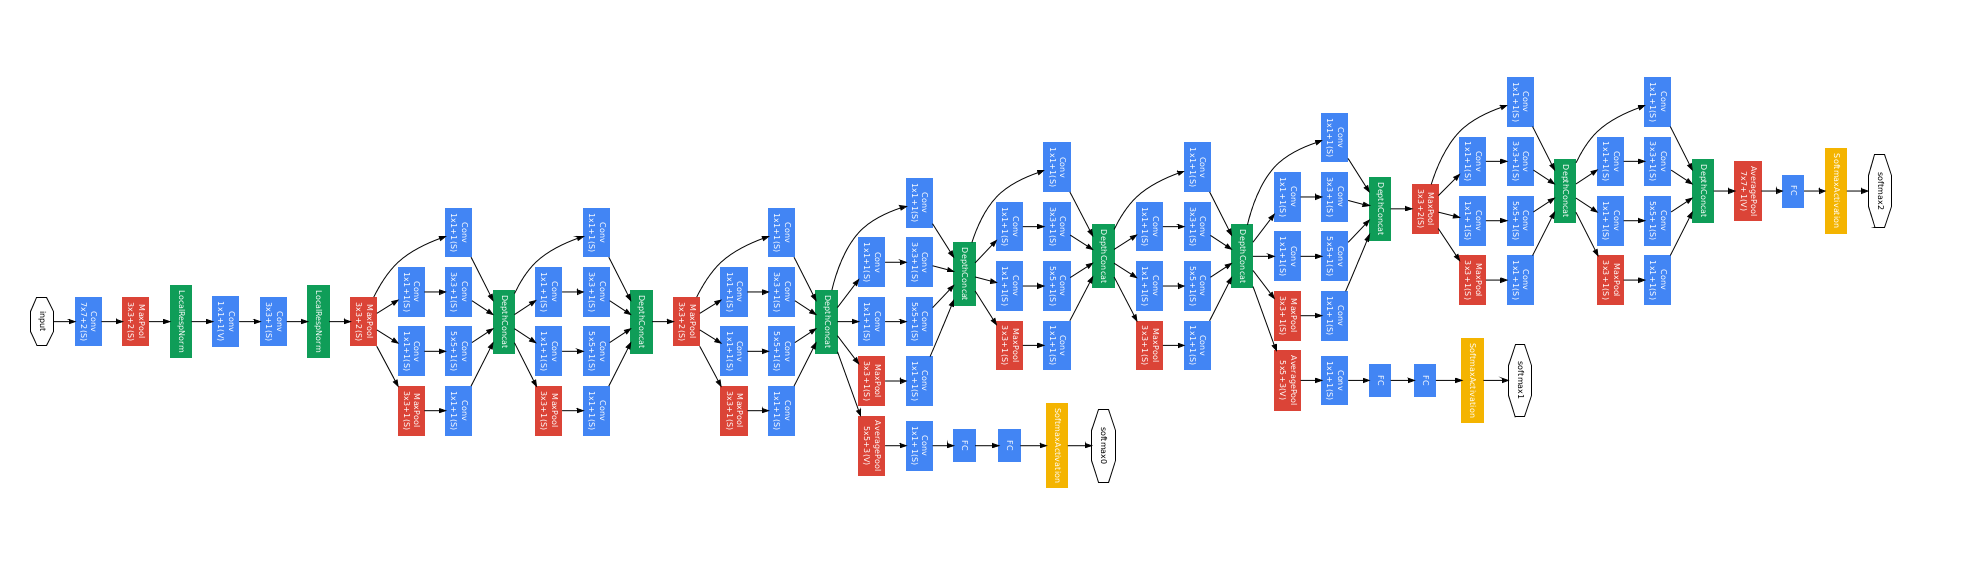
\includegraphics[width=\textwidth]{figure5}
    \caption{Kiến trúc của mạng GoogLeNet có 22 khối Convolutional, mỗi khối bao gồm một nhiều lớp.}
\end{figure}

\subsubsection{Hàm kích hoạt}

Hàm kích hoạt thể hiện trạng thái kích hoạt đầu ra của nơ-ron. Hàm kích hoạt có thể là hàm tuyến tính (hàm đồng nhất $ f(x) = x $) ở lớp cuối cùng, nếu mạng được luyện tập để giải bài toán regression. Tuy nhiên, chỉ có các hàm kích hoạt phi tuyến tính mới cho phép mạng nơ-ron biểu diễn các mối quan hệ phức tạp. Điều này có thể dễ dàng chứng minh được từ công thức của mạng kết nối đầy đủ:

Với hai lớp mạng $ Y_1 = f_1(W_1x) $ và $ Y_2 = f_2(W_2x) $ xếp kế tiếp nhau, $ f_1(x) $ là hàm tuyến tính có dạng $ f_1(x) = Cx $, ta có:
$$ Y_2(x) =  f_2z_2 = f_2(W_2f_1(W_1x)) = f_2((W_2CW_1)x) $$

Nói cách khác, phép tính toán qua hai lớp mạng sử dụng hàm kích hoạt tuyến tính có thể giản lược được thành một lớp duy nhất, không hề làm tăng độ phức tạp của mô hình.

Một số hàm kích hoạt tiêu biểu có thể kể đến:
\begin{itemize}
    \item Hàm sigmoid: $ \cfrac{1}{1 + e^{-x}} $. Hàm sigmoid được sử dụng trong thuật toán logistic regression để giới hạn output trong khoảng $ (0, 1) $, thể hiện giá trị dự đoán false-true.
    \item Hàm tanh: $ \cfrac{e^{x} + e^{-x}}{e^{x} - e^{-x}} $. Giá trị đầu ra của hàm tanh nằm trong khoảng $ (-1, 1) $, giúp ta đưa chuẩn hóa giá trị đầu ra kì vọng về 0.
    \item Hàm ReLU: $ max\{x, 0\} $. Khác với sigmoid và tanh, hàm ReLU có công thức tính toán vô cùng đơn giản và dễ lấy đạo hàm, giúp tăng tốc quá trình luyện tập.
    \item Hàm Leaky ReLU: $ max\{x, \alpha x\} $. Khi giá trị của $ x $ về âm, hàm ReLU cơ bản có đạo hàm bằng 0, dẫn tới việc chết gradient và ngăn cản quá trình luyện tập. Leaky ReLU là một phiên bản cải tiến giúp giải quyết vấn đề này.
\end{itemize}

\subsection{Mạng nơ-ron tích chập (Convolutional Neural Network)}

Tuy mạng nơ-ron kết nối đầy đủ có thể dễ dàng biểu diễn mối quan hệ giữa mọi nơ-ron với nhau, số lượng tham số khổng lồ khiến cho việc tính toán vô cùng khó khăn. Giữa hai lớp mạng có $ n $ và $ m $ nơ-ron, ta cần ma trận trọng số $ W $ với $ (n + 1) \times m $ phần tử. Đây là một trở ngại đặc biệt lớn đối với dữ liệu hình ảnh - một bức ảnh HD có kích thước $ 1280 \times 720 $ pixel, tương ứng với gần 1 triệu giá trị đầu vào. Xây dựng ma trận trọng số $ W $ đầy đủ cho dữ liệu đầu vào này là điều không thể.

Quan sát dữ liệu hình ảnh, ta nhận thấy các pixel ở gần thường có quan hệ chặt chẽ với nhau hơn là các pixel ở xa. Do đó, ta không nhất thiết phải biểu diễn quan hệ giữa tất cả các pixel với nhau - chỉ cần tìm ra quan hệ giữa các cụm pixel ở gần nhau trên ảnh là đủ. Mạng nơ-ron tích chập (Convolutional Neural Network hay CNN) được xây dựng dựa trên tư tưởng này.

\subsubsection{Lớp tích chập}
\label{convolutional-layer}

Với ma trận ảnh đen trắng kích thước $ n \times n $:
\begin{center}
    \begin{math}
        x = \begin{bmatrix}
            x_{1,1}, x_{1,2},..., x_{1,n} \\
            x_{2,1}, x_{2,2},..., x_{2,n} \\
            ...                           \\
            x_{n,1}, x_{n,2},..., x_{n,n} \\
        \end{bmatrix}
    \end{math}
\end{center}
\begin{figure}[H]
    \centering
    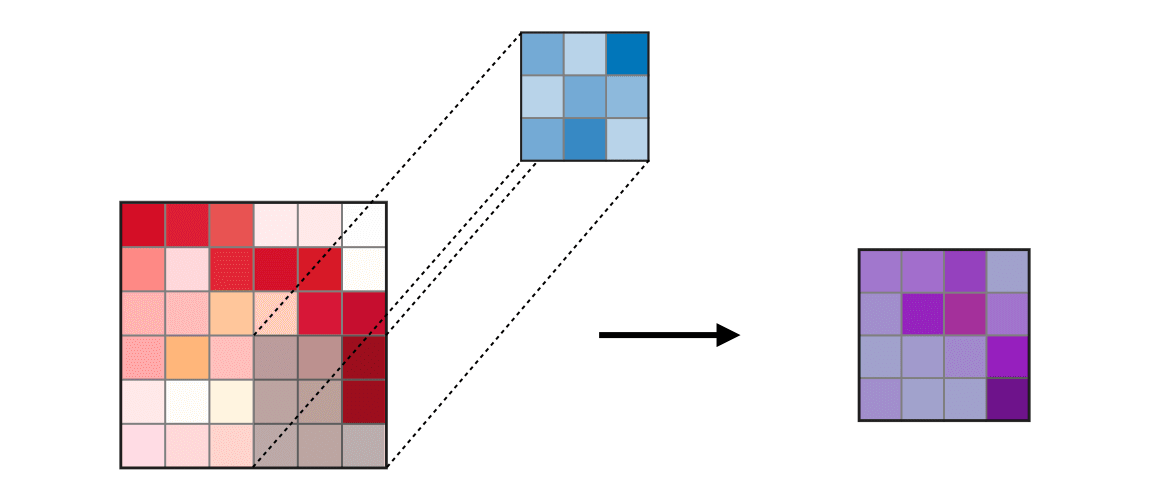
\includegraphics[width=0.7\textwidth]{figure6}
    \caption{Cơ chế hoạt động của kernel. Nguồn ảnh: \cite{CS230}}
\end{figure}
ta định nghĩa kernel là một ma trận kích thước nhỏ $ m \times m $:
\begin{center}
    \begin{math}
        k = \begin{bmatrix}
            k_{1,1}, k_{1,2},..., k_{1,m} \\
            k_{2,1}, k_{2,2},..., k_{2,m} \\
            ...                           \\
            k_{m,1}, k_{m,2},..., k_{m,m} \\
        \end{bmatrix}
    \end{math}
\end{center}
và phép toán tích chập $ x \circledast k $ cho ra ma trận kết quả $ x' $, kích thước $ (n - m + 1) \times (n - m + 1) $, với:
$$ x'_{u,v} = \sum_{i=0}^{m-1} \sum_{j=0}^{m-1} x_{u+i,v+j} \cdot k_{i+1,j+1} $$

Bằng cách lựa chọn trọng số phù hợp, phép tích chập với kernel có thể thực hiện được nhiều thao tác xử lý ảnh như làm mờ, làm sắc ảnh, nhận diện cạnh,\dots Qua đó, kernel đóng vai trò như bộ lọc thông tin, tìm ra các đặc điểm hữu ích từ dữ liệu.

\begin{figure}[H]
    \centering
    \begin{subfigure}[H]{0.35\textwidth}
        \centering
        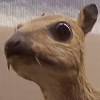
\includegraphics[width=0.5\linewidth]{figure7.png}
        \caption{Ảnh gốc}
    \end{subfigure}
    \begin{subfigure}[H]{0.25\textwidth}
        \centering
        \begin{math}
            \begin{bmatrix}
                -1, -1, -1 \\
                -1, 8, -1  \\
                -1, -1, -1
            \end{bmatrix}
        \end{math}
        \caption{Kernel}
    \end{subfigure}
    \begin{subfigure}[H]{0.35\textwidth}
        \centering
        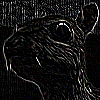
\includegraphics[width=0.5\linewidth]{figure8.png}
        \caption{Kết quả}
    \end{subfigure}
    \caption{Nhận diện cạnh bằng kernel}
\end{figure}

Trên thực tế, ta thường làm việc với dữ liệu ảnh có nhiều kênh (channel), ví dụ ảnh RGB có 3 kênh biểu diễn giá trị màu đỏ - xanh lá - xanh lam. Kernel cho dữ liệu dạng này cũng có số channel tương ứng, và phép tích chập được thực hiện trên tất cả các chiều.

Mạng CNN sử dụng các lớp tích chập (convolutional), mỗi lớp được cấu thành bởi nhiều kernel. Lớp tích chập nhận vào dữ liệu có nhiều kênh (thường là dữ liệu ảnh) và trả về kết quả cũng có nhiều kênh, mỗi kênh là kết quả tích chập với một kernel. Kết quả này có thể được sử dụng bởi các lớp tích chập hoặc kết nối đẩy đủ kế tiếp. Quá trình luyện tập hướng tới việc học ra trọng số tốt nhất cho cả các kernel và ma trận kết nối đầy đủ.

Lớp tích chập có thể được tinh chỉnh bằng một số tham số:
\begin{itemize}
    \item Kích thước các chiều và số kênh của dữ liệu đầu vào. Đối với dữ liệu ảnh RGB, ta có hai chiều rộng $ W $ và cao $ H $, số kênh $ C = 3 $. Ta thường sử dụng ảnh vuông với $ W = H $.
    \item Kích thước các chiều của kernel. Ta cũng thường sử dụng kernel vuông với kích thước hai chiều $ K $ nhỏ, không vượt quá 7.
    \item Số lượng kernel $ C' $. Giá trị này thường là số mũ của 2, và tăng dần ở các lớp sau của mô hình.
    \item Bước nhảy (stride) $ S $ của phép tích chập. Lớp sẽ tính tích chập của các cụm phần tử cách nhau $ S $ bước. Đối với phép tích chập cơ bản, $ S = 1 $.
    \item Kích thước đệm (padding) $ P $ cho ma trận đầu vào. Bằng cách đệm xung quanh ma trận đầu vào (thường là bằng giá trị 0), ta có thể điều chỉnh kích cỡ ma trận đầu ra. Đối với phép tích chập cơ bản, $ P = 0 $.
    \item Hàm kích hoạt. Do phép tích chập là phép toán tuyến tính, hàm kích hoạt đóng vai trò tương tự như đối với lớp kết nối đầy đủ.
\end{itemize}

Với các tham số trên, lớp tích chập có tất cả $ C' \times C \times K \times K $ tham số, cho ra đầu ra kích thước $ C' \times W' \times H' $, với $ W' = H' = \cfrac{W - K + 2P}{S} + 1 $. Số lượng tham số của lớp tích chập chỉ phụ thuộc vào số kênh của dữ liệu đầu vào (thường là nhỏ), giúp giảm đáng kể kích thước của mô hình mà vẫn đảm bảo thực hiện được những tính toán phức tạp.

\subsubsection{Lớp pooling}

Tuy số lượng tham số của lớp tích chập rất nhỏ, song kích thước đầu ra vẫn còn rất lớn, khiến việc tính toán còn khó khăn. Để giảm kích thước đầu ra mà vẫn giữ được những thông tin quan trọng, ta sử dụng lớp pooling ở giữa các lớp tích chập.

\begin{figure}[H]
    \centering
    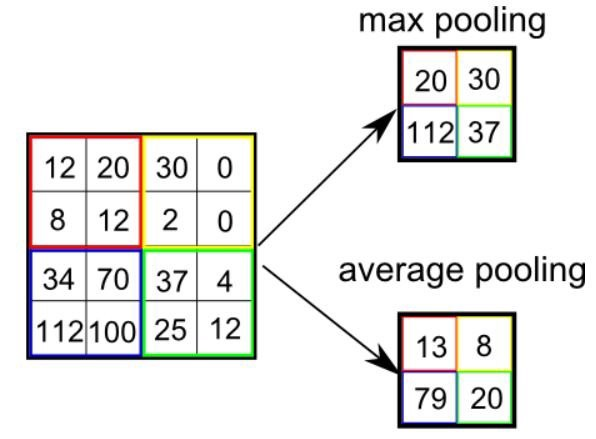
\includegraphics[width=0.7\textwidth]{figure9.jpg}
    \caption{Cơ chế hoạt động của Max pooling và Average pooling với size 2, stride 2}
\end{figure}

Lớp pooling tổng hợp giá trị của các vùng lân cận trên dữ liệu bằng phép lấy max hoặc phép tính trung bình thành để cho ra một kết quả đầu ra duy nhất. Lớp pooling có thể tùy chỉnh được bằng hai tham số kích thước và bước nhảy, giống như với các lớp tích chập. Một lớp pooling có kích thước $ K = 2 $, bước nhảy $ S = 2 $ sẽ giảm được một nửa kích thước mỗi chiều của dữ liệu:
$$  W' = H' = \cfrac{W - 2}{2} + 1 = \cfrac{W}{2} $$

Lớp pooling không có tham số cần học.

\subsection{Hàm mục tiêu và thuật toán huấn luyện}

\subsubsection{Bài toán huấn luyện mô hình mạng nơ-ron}

Như đã chỉ ra trong các mục trên, mục tiêu của quá trình huấn luyện mạng nơ-ron là tìm ra trọng số cho các lớp mạng để mạng hoạt động tốt nhất. Gọi tập hợp trọng số của mạng nơ-ron là $ W $, ta viết lại yêu cầu này thành bài toán tối ưu:
$$ minimize \; J(W) \; \forall \; W \in R^{n} $$

$ J(W) $ được gọi là hàm mục tiêu hoặc hàm thiệt hại (loss function), có chức năng đánh giá sai số của mô hình so với kết quả kì vọng. Tùy vào mục đích của bài toán mà ta lựa chọn hàm mục tiêu khác nhau. Hai hàm mục tiêu tiêu biểu có thể kể đến là:
\begin{itemize}
    \item Sai số toàn phương trung bình (Mean Square Error hay MSE): $ \cfrac{1}{n} \sum_{i=1}^{n} (Y_i - \hat{Y}_i)^2 $, với $ n $ là kích thước bộ dữ liệu, $ Y_i $ và $ \hat{Y}_i $ là giá trị đầu ra thực tế và đầu ra của mô hình. Hàm mục tiêu này được sử dụng cho các mô hình regression.
    \item Hàm cross entropy: $ - \sum_{i=1}^{n} \sum_{j=1}^{m} Y_{i, j} \log(\hat{Y}_{i, j}) $, với $ n $ là kích thước bộ dữ liệu, $ m $ là số lượng lớp của bài toán phân loại, $ Y_i $ và $ \hat{Y}_i $ là giá trị đầu ra thực tế và đầu ra của mô hình. Hàm mục tiêu này được sử dụng cho các mô hình phân loại.
\end{itemize}

Một mô hình học sâu hiện đại có thể có hàng chục triệu, thậm chí hàng trăm triệu, hàng tỷ tham số. Miền tìm kiếm của hàm mục tiêu vì thế cũng vô cùng lớn, không thể tính toán trực tiếp để giải ra giá trị cực tiểu được. Thay vào đó, ta sử dụng các thuật toán tối ưu tuần tự: xuất phát từ một lời giải ngẫu nhiên trong miền tìm kiếm, các thuật toán này sẽ dần cập nhật lời giải tốt dần lên cho tới khi hội tụ ở giá trị cực tiểu địa phương.

\subsubsection{Thuật toán xuống đồi cổ điển}

Thuật toán xuống đồi cổ điển (Stochastic Gradient Descent) là thuật toán tối ưu tuần tự cơ bản nhất - từ vị trí lời giải hiện tại, di chuyển ngược chiều gradient của hàm mục tiêu một đoạn nhỏ ("xuống đồi") để tìm lời giải mới. Tốc độ học (learning rate) $ \alpha $ quyết định độ dài bước nhảy xuống đồi và được chỉ định bởi người dùng.

Để có thể tính toán nhanh gradient của hàm mục tiêu theo tất cả các tham số, ta sử dụng thuật toán dẫn truyền ngược backpropagation. Cho hai lớp mạng kế tiếp nhau $ Y_1 $ và $ Y_2 $. Vì phép nhân ma trận của mạng kết nối đầy đủ và phép tích chập của mạng CNN đều là phép toán tuyến tính, ta có thể viết lại công thức của hai lớp mạng này thành:
$$ Y_1 = f_1(z_1) = f_1(W_1x) $$
$$ Y_2 = f_2(z_2) = f_2(W_2Y_1) $$
với $ f_1(x) $ và $ f_2(x) $ là hàm kích hoạt.

Theo quy tắc chuỗi đạo hàm, ta có:
\begin{align*}
    \cfrac{\delta J(W)}{\delta W_2} & = \cfrac{\delta J(W)}{\delta z_2} \times \cfrac{\delta z_2}{\delta W_2} \\
                                    & = \cfrac{\delta J(W)}{\delta z_2} \times Y_1
\end{align*}
và:
\begin{align*}
    \cfrac{\delta J(W)}{\delta z_2} & = \cfrac{\delta J(W)}{\delta Y_2} \times \cfrac{\delta Y_2}{\delta z_2}      \\
                                    & = \cfrac{\delta J(W)}{\delta Y_2} \times \cfrac{\delta f_2(z_2)}{\delta z_2}
\end{align*}

Giả sử $ Y_2 $ là lớp đầu ra của mô hình, ta có:
\begin{itemize}
    \item $ Y_1 $ là kết quả đầu ra của lớp liền trước nó.
    \item $ \cfrac{\delta J(W)}{\delta Y_2} $ là đạo hàm của hàm mục tiêu theo kết quả dự đoán.
    \item $ \cfrac{\delta f_2(z_2)}{\delta z_2} $ là đạo hàm của hàm kích hoạt $ f_2(x) $ tại $ x = z_2 $.
\end{itemize}

Nói cách khác, nếu có công thức đạo hàm của hàm mục tiêu và hàm kích hoạt, ta có thể nhanh chóng tính được đạo hàm thành phần của các trọng số lớp cuối cùng.

Tương tự, ta có thể tính được đạo hàm thành phần của lớp liền trước, sử dụng công thức đạo hàm của hàm kích hoạt:
\begin{align*}
    \cfrac{\delta J(W)}{\delta W_l} & = \cfrac{\delta J(W)}{\delta z_l} \times \cfrac{\delta z_l}{\delta W_l} \\
                                    & = e_l \times Y_{l - 1}
\end{align*}
với:
\begin{align*}
    e_l = \cfrac{\delta J(W)}{\delta z_l} & = \cfrac{\delta J(W)}{\delta z_{l + 1}} \times \cfrac{\delta z_{l + 1}}{\delta Y_l} \times \cfrac{\delta Y_l}{\delta z_l} \\
                                          & = e_{l + 1} \times W_{l + 1} \times \cfrac{\delta f_{l + 1}(z_l)}{\delta z_l}
\end{align*}
Tiếp tục như vậy, ta tính được đạo hàm thành phần cho trọng số của tất cả các lớp mạng. Tên của thuật toán backpropagation cũng giải thích cơ chế hoạt động của nó - ta tìm gradient của mạng từ lớp cuối cùng tới lớp đầu tiên, ngược với quá trình tính toán hàm mục tiêu đi từ lớp đầu tới lớp cuối.

\begin{algorithm}[H]
    \caption{Thuật toán backpropagation}
    \begin{algorithmic}[1]
        \Procedure{backprop}{mạng nơ-ron $ l $ lớp, $ J(x) $}
        \State $ e_l \gets \cfrac{\delta J(W)}{\delta \hat{Y}} \times \cfrac{\delta f_l(z_l)}{\delta z_m} $
        \State $ \cfrac{\delta J(W)}{\delta W_l} = e_l \times Y_{l - 1} $
        \For{i từ $ l - 1 $ tới 1}
        \State $ e_i = e_{i + 1} \times W_{i + 1} \times \cfrac{\delta f_{i + 1}(z_i)}{\delta z_i} $
        \State $ \cfrac{\delta J(W)}{\delta W_i} = e_i \times Y_{i - 1} $
        \EndFor
        \State \textbf{return} $ \cfrac{\delta J(W)}{\delta W} $
        \EndProcedure
    \end{algorithmic}
\end{algorithm}

\begin{algorithm}[H]
    \caption{Thuật toán xuống đồi cổ điển}
    \begin{algorithmic}[1]
        \Procedure{SGD}{mạng nơ-ron, $J(x), \alpha, epochs$}
        \State Khởi tạo $ W $ ngẫu nhiên.
        \For{i từ 1 tới $ epochs $}
        \State Tính $ J(W) $, lưu lại giá trị output của các lớp
        \State $ gradient \gets \text{BACKPROP}(\text{mạng nơ-ron}, J(x)) $
        \State $ W \gets W - \alpha \times gradient $
        \EndFor
        \State \textbf{return} $ W $
        \EndProcedure
    \end{algorithmic}
\end{algorithm}

Tốc độ học của thuật toán xuống đồi ảnh hưởng trực tiếp tới chất lượng của mô hình được huấn luyện. Nếu tốc độ học quá nhỏ, thuật toán phải mất một thời gian dài mới có thể hội tụ. Nếu tốc độ học quá lớn, bước nhảy của thuật toán có thể bỏ qua cực tiểu địa phương, thậm chí càng lúc càng bỏ xa cực tiểu, dẫn tới mô hình không bao giờ hội tụ. Để khắc phục hiện tượng này, ta có thể sử dụng kĩ thuật learning rate decay - bắt đầu huấn luyện từ một giá trị learning rate cao để xuất phát nhanh, và giảm dần qua thời gian khi mô hình đã ổn định, cần bước tinh chỉnh nhỏ.

\begin{figure}[H]
    \centering
    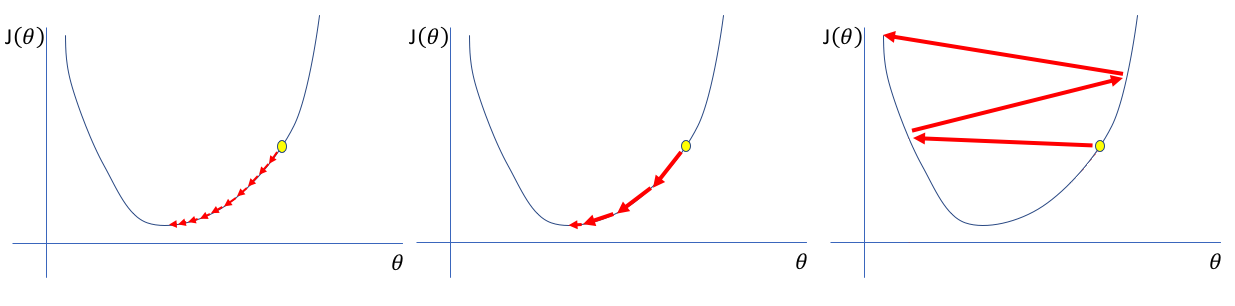
\includegraphics[width=\textwidth]{figure11.png}
    \caption{Ảnh hưởng của việc lựa chọn tốc độ học đối với việc huấn luyện mô hình. Từ trái qua: mô hình có tốc độ học quá nhỏ, hội tụ chậm; mô hình có tốc độ học vừa phải; mô hình có tốc độ học quá lớn, dẫn tới không thể hội tụ.}
\end{figure}

Trên thực tế, các bộ dữ liệu được dùng để tối ưu mô hình học máy có thể có kích cỡ lên tới hàng triệu, hàng chục triệu phần tử. Khả năng tính toán của phần cứng hiện tại không cho phép ta trực tiếp tính gradient cho toàn bộ bộ dữ liệu cùng một lúc. Thay vào đó, ta chia bộ dữ liệu thành các lô (batch) nhỏ, vừa bộ nhớ để tính toán. Gradient lúc này được lấy theo trung bình của lô, thay vì của toàn bộ bộ dữ liệu - điều này khiến cho lời giải không thể di chuyển thẳng theo hướng gradient thực, giá trị hàm thiệt hại không giảm liên tục, và thuật toán có thể không hội tụ chặt tới cực tiểu địa phương. Tuy nhiên, thuật toán tối ưu theo lô nhìn chung vẫn thực hiện tốt nhiệm vụ tối ưu mô hình.

\subsubsection{Các thuật toán tối ưu cải tiến}

Thuật toán xuống đồi cổ điện sẽ gặp khó khăn nếu hàm mục tiêu chịu ảnh hưởng bởi một số biến nhiều hơn các biến khác khác, do giá trị lời giải phải liên tục di chuyển qua lại trong vùng "thung lũng", thay vì tập trung vào hướng đi có tốc độ giảm lớn nhất. Để khắc phục nhược điểm này, Ning Qian đề xuất kĩ thuật momentum (quán tính) \cite{QIAN1999145} - không sử dụng trực tiếp gradient, thay vào đó cập nhật lời giải hiện tại bằng vector:
$$ v_t = \gamma v_{t-1} - \alpha \nabla_{W} J(W)  $$
với $ v_t $ là vector cập nhật ở bước duyệt thứ $ t $, $ \gamma $ là hệ số momentum, thường mang giá trị trong khoảng $ [0.9, 1) $. Việc xây dựng vector cập nhật tích lũy dần như vậy giúp thuật toán có thể bám theo hướng đi tốt đã biết từ trước (quán tính) thay vì đột ngột chuyển hướng ngẫu nhiên.

\begin{figure}[H]
    \centering
    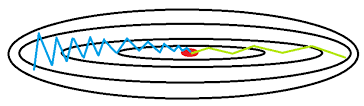
\includegraphics[width=0.5\textwidth]{figure12.png}
    \caption{So sánh giữa việc tối ưu sử dụng thuật toán cổ điển (đường xanh dương) với tối ưu sử dụng momentum (đường xanh lá.)}
\end{figure}

Thuật toán xuống đồi cổ điển cũng sử dụng chung một tốc độ học cho toàn bộ mạng. Nếu dữ liệu không được phân bố đều - ví dụ, khi một số đặc tính phổ biến hơn các đặc tính khác, các trọng số liên quan sẽ không được cập nhật đều nhau, dẫn tới việc mô hình không học được đầy đủ thông tin. Dean, J., Corrado và cộng sự khắc phục hạn chế này bằng kĩ thuật Adagrad (ADAptive GRADient) để điều chỉnh tốc độ học độc lập cho từng tham số \cite{duchi2011adaptive}:

Đặt $ g_{t, i} = \nabla_{W_i} J(W) $ tại thời điểm $ t $, $ G_{t, i} = \sum_{u = 1}^{t} g_{u, i}^2 $, ta có công thức của bước cập nhật thứ $ t + 1 $ là:

$$ W_{t + 1, i} = W_{t, i} - \cfrac{\alpha}{\sqrt{G_{t, i} + \epsilon}} \times g_{t, i}  $$

$ \epsilon $ là một giá trị dương cực nhỏ để tránh xảy ra hiện tượng chia cho 0.

Từ công thức trên, dễ thấy các tham số được cập nhật thường xuyên sẽ có tổng $ G_{t, i} $ lớn hơn, khiến cho các bước cập nhật kế tiếp trở nên nhỏ và ít hiệu lực hơn. Ngược lại, nếu một tham số không được cập nhật thường xuyên, tổng $ G_{t, i} $ của nó sẽ nhỏ hơn, và tham số đó sẽ được tập trung tối ưu hơn trong các bước kế tiếp. Adagrad loại bỏ nhu cầu cần phải cập nhật tốc độ học bằng tay, thay vào đó tốc độ học được tự động tối ưu trong quá trình chạy. Nhược điểm của Adagrad là khi số lượng bước lặp càng lớn, tổng $ G_{t, i} $ càng lớn, dẫn tới triệt tiêu hoàn toàn gradient và dừng quá trình học.

Để khắc phục nhược điểm triệt tiêu gradient, các biến thể của Adagrad chỉ điều chỉnh tốc độ học sử dụng một phần tổng bình phương gradient, thay vì sử dụng toàn bộ tổng tích lũy. Một trong những biến thể hay được sử dụng là RMSprop, được đề xuất bởi Geoff Hinton:
$$ E[g^2]_t = \gamma E[g^2]_{t - 1} + (1 - \gamma) g_t^2 $$
$$ W_{t + 1, i} = W_{t, i} - \cfrac{\alpha}{\sqrt{E[g^2]_t + \epsilon}} \times g_{t, i} $$

Tổng có trọng số $ E[g^2]_t $ đảm bảo chỉ các gradient mới nhất có ảnh hưởng lớn tới tốc độ học của tham số, ngăn không cho gradient bị biến mất khi $ t \to +\infty $. Hinton đề xuất sử dụng giá trị $ \gamma = 0.9 $.

Thuật toán tối ưu được sử dụng trong báo cáo tốt nghiệp này là thuật toán Adam (ADAptive Moment Estimation) \cite{kingma2017adam}, là sự kết hợp của hai phương pháp momentum và RMSprop:
\begin{align*}
    m_t       & = \beta_1m_{t - 1} + (1 - \beta_1) g_t                        \\
    v_t       & = \beta_1v_{t - 1} + (1 - \beta_1) g_t^2                      \\
    \hat{m_t} & = \cfrac{m_t}{1 - \beta_1^t}                                  \\
    \hat{v_t} & = \cfrac{v_t}{1 - \beta_2^t}                                  \\
    W_{t + 1} & = W_t - \cfrac{\alpha}{\sqrt{\hat{v_t}} + \epsilon} \hat{m_t}
\end{align*}

Hai giá trị $ \hat{m_t} $ và $ \hat{v_t} $ được sử dụng thay cho  $ m_t $ và  $ v_t $ để khắc phục tình trạng thuật toán xuất phát chậm trong các vòng lặp đầu tiên.

\section{Generative Adversarial Network (GAN)}

Khả năng ước lượng hàm phức tạp với độ chính xác cao của các mô hình học sâu có giám sát mở ra nhiều hướng nghiên cứu triển vọng trong lĩnh vực trí tuệ nhân tạo. Generative Adversarial Network - mạng đối nghịch tạo sinh, gọi tắt là GAN - là một trong số đó.

\subsection{Định nghĩa}

GAN được đề xuất lần đầu tiên bởi Ian Goodfellow và cộng sự vào năm 2014 \cite{NIPS2014_5ca3e9b1}. Một mô hình GAN cơ bản bao gồm hai phần:

\begin{itemize}
    \item Một mạng sinh dữ liệu (generator). Generator thường nhận vào một vector ngẫu nhiên - gọi là vector biểu diễn tiềm thức (latent vector) - và cho ra một dữ liệu giả tương ứng với vector đó.
    \item Một mạng phân loại dữ liệu (discriminator). Discriminator thường nhận vào dữ liệu thật hoặc dữ liệu giả của generator, và cho ra kết quả phân loại dữ liệu này là thật hay giả.
\end{itemize}

Hai mạng này được tối ưu song song để chống lại nhau - Output của generator được đưa làm input của discriminator để luyện tập phân biệt thật/giả. Ngược lại, generator luyện tập để có thể sinh dữ liệu giả đánh lừa được discriminator. Ban đầu, generator chỉ có thể cho ra kết quả giả, song qua thời gian, generator dần học được cách để tạo ra dữ liệu có thể đánh lừa discriminator. Tương tự, discriminator cũng phải dần học cách đối phó với năng lực của generator. Mục tiêu cuối cùng của GAN là xây dựng được generator chất lượng cao, sinh được dữ liệu với phân bố giống với dữ liệu thật, khiến cho discriminator phải dự đoán ngẫu nhiên và đánh lừa được cả con người.

\begin{figure}[H]
    \centering
    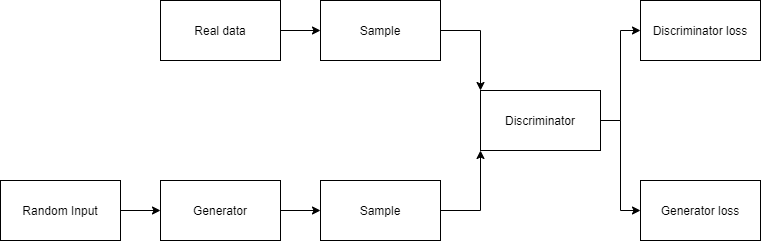
\includegraphics[width=\textwidth]{figure13.png}
    \caption{Kiến trúc GAN cơ bản}
\end{figure}

\subsection{Luyện tập mô hình GAN}
\label{gan}

Quá trình luyện tập GAN liên tục hoán đổi giữa hai bước:
\begin{enumerate}
    \item Thực hiện một hoặc nhiều bước tối ưu discriminator, giữ nguyên các trọng số của generator.
    \item Thực hiện một hoặc nhiều bước tối ưu generator, giữ nguyên các trọng số của discriminator.
\end{enumerate}

Hàm mục tiêu sử dụng để tối ưu hai thành phần của GAN có thể là các hàm mục tiêu của mô hình học có giám sát - trong bài báo giới thiệu GAN, Ian Goodfellow sử dụng hàm thiệt hại Minimax, về cơ bản là một biến thể của hàm cross entropy:
$$ E_x[\log(D(x))] + E_z[\log(1 - D(G(z)))] $$
với $ E_x $ là giá trị kì vọng trên toàn bộ tập dữ liệu thật, $ E_z $ là giá trị vì vọng trên toàn bộ tập dữ liệu giả, $ G(z) $ và $ D(x) $ lần lượt là kết quả đầu ra của mạng generator và discriminator. Generator cố gắng tối giảm hàm thiệt hại này, trong khi discriminator lại cố gắng tối đa; chính vì lí do đó mà hàm thiệt hại này được gọi là Minimax - đây là một trò chơi minimax giữa hai tác tử.

Ta giữ nguyên trọng số của generator khi tối ưu discriminator, vì mục tiêu của discriminator là học được các thiếu sót của dữ liệu giả, khác với mục tiêu của generator. Tri thức discriminator học được trong giai đoạn này không giúp cho generator hoạt động tốt lên. Ngược lại, ta giữ nguyên trọng số của discriminator khi cập nhật generator, để mô hình này có thể hội tụ tới một mục tiêu cố định.

Khác với mô hình học có giám sát hội tụ ở điểm cực tiểu địa phương, ta không thể xác định được thời điểm GAN hội tụ. Một khi generator trở nên đủ tốt để đánh lừa discriminator, discriminator buộc phải đưa ra dự đoán ngẫu nhiên để phân loại dữ liệu thật/giả. Điều này dẫn tới việc generator cũng bị cập nhật dựa trên các tri thức không có giá trị, khiến cho chất lượng đầu ra đi xuống. Do đó, GAN không thể duy trì trạng thái hội tụ lâu dài.

Một vấn đề khác khiến cho việc luyện tập mô hình GAN trở nên khó khăn là hiện tượng mode collapse. Hiện tượng này xảy ra khi generator tập trung sinh ra một số rất ít dữ liệu tốt để đánh lừa discriminator, hoàn toàn bỏ qua tính đa dạng. Trong trường hợp này, hướng đi tốt nhất đối với discriminator là gắn nhãn tất cả các dữ liệu bị lặp lại thành dữ liệu giả, tuy nhiên điều này có thể không xảy ra nếu mạng bị mắc kẹt ở cực tiểu địa phương. Một số phương án được đề xuất để đối phó với tình trạng này bao gồm hàm mục tiêu Wasserstein và Unrolled GANs.

\section{Vấn đề bias-variance trade off}

\subsection{Định nghĩa}

Khi xây dựng các mô hình học có giám sát, sai số có thể xuất hiện dưới hai dạng: bias và variance.

\begin{itemize}
    \item Sai số bias xuất hiện khi mô hình đưa ra những giả thiết không chính xác về dữ liệu đầu vào. Khi bias cao, mô hình có thể không mô tả được mối tương quan giữa đầu vào và đầu ra (underfitting).
    \item Sai số variance xuất hiện khi mô hình bám quá sát vào dữ liệu đầu vào. Khi variance cao, mô hình có thể không hoạt động tốt với những dữ liệu mới chưa từng gặp trước đó (overfitting).
\end{itemize}

Mô hình học máy lý tưởng có thể mô phỏng chính xác mối tương quan giữa dữ liệu đầu vào và đầu ra mẫu (bias thấp), đồng thời cũng phải hoạt động tốt với dữ liệu mới (variance thấp).

\begin{figure}[H]
    \centering
    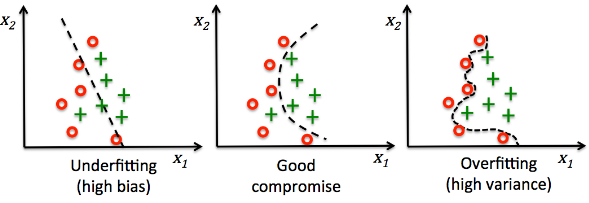
\includegraphics[width=0.7\textwidth]{figure2}
    \caption{Với cùng một bộ dữ liệu, mô hình có bias cao không thể mô phỏng chính xác mối quan hệ giữa đầu vào và đầu ra. Mô hình có variance cao quá phức tạp và dễ sai khi gặp phải dữ liệu mới. Mô hình ở giữa ở mức độ cân bằng chấp nhận được.}
\end{figure}

Tuy nhiên, thực tế thường khó thực hiện được cả hai mục tiêu này. Nếu sử dụng những mô hình học máy phức tạp, ta có thể dễ dàng biểu diễn được sự liên hệ của dữ liệu mẫu, song lại có nguy cơ overfitting và hoạt động kém với dữ liệu ngoài. Mô hình đơn giản hơn có thể khái quát hóa lời giải tốt hơn, nhưng lại không đủ để biểu diễn các quan hệ thực tế phức tạp.

Vấn đề bias-variance trade off mô tả mâu thuẫn khi hai loại sai số trong các mô hình học máy bù trừ cho nhau, và giảm được một sai số thường dẫn tới việc tăng sai số còn lại. Việc tìm ra điểm cân bằng giữa bias và variance là vô cùng quan trọng để xây dựng được một mô hình học máy tốt.

\subsection{Phương hướng giải quyết}

Trên thực tế, chúng ta thường quan tâm giải quyết vấn đề overfitting hơn, vì:
\begin{enumerate}
    \item Underfitting có thể dễ dàng nhận ra được, do mô hình không hoạt động tốt ngay từ trong quá trình luyện tập. Overfitting chỉ có thể bị phát hiện khi đánh giá mô hình với dữ liệu mới.
    \item Các mô hình học máy hiện đại, đặc biệt là các mô hình học sâu (Deep Learning) có xu hướng càng ngày càng phức tạp, và do đó càng dễ mắc phải tình trạng overfitting.
\end{enumerate}

Các phương pháp phòng tránh overfitting thường hướng tới (1) kiểm tra khả năng khái quát hóa và (2) kiểm soát độ phức tạp của mô hình. Đối với các mô hình mạng nơ-ron, một số phương án phổ biến có thể kể đến:

\subsubsection{Cross-validation}

Kĩ thuật cross-validation (kiểm chứng chéo) phân chia bộ dữ liệu thành hai phần - một bộ dữ liệu luyện tập (training set) và một bộ dữ liệu kiểm chứng (validation set). Mô hình sau khi đã được luyện tập trên training set sẽ được kiểm tra trên validation set để kiểm tra chất lượng với dữ liệu chưa được gặp.

Để giảm thiểu nhiễu trong tập kiểm chứng, phần lớn kĩ thuật kiểm chứng chéo sẽ thực hiện nhiều vòng kiểm tra, mỗi vòng phân chia dữ liệu thành các phần khác nhau. Kết quả các vòng được tính trung bình để cho ra đánh giá cuối cùng.

\subsubsection{Regularization}

Kĩ thuật regularization bổ sung thêm hàm số regularization vào hàm mục tiêu, đánh vào độ phức tạp của mô hình. Tối ưu hàm regularization sẽ ép một số trọng số về 0 - nói cách khác, mạng nơ-ron phải chọn giữ lại những trọng số quan trọng nhất, tránh việc phức tạp hóa dẫn tới overfitting.

Gọi $ W $ là vector trọng số của mạng, ta có công thức của hai hàm số regularization phổ biến:

\begin{itemize}
    \item Ridge Regression: $ \sum W_i^2 $
    \item Lasso: $ \sum |W_i| $
\end{itemize}

\subsubsection{Dropout}

Khi luyện tập mạng nơ-ron sử dụng kĩ thuật dropout, một số giá trị đầu ra sẽ bị bỏ qua (đặt về 0) một cách ngẫu nhiên với xác suất $ p $. Điều này ép các lớp trong mạng nơ-ron phải học cách tận dụng đa dạng thông tin khác nhau từ lớp trước, thay vì phụ thuộc vào một số ít thông tin cụ thể, có thể dễ dàng biến mất do dropout. Qua đó, ta giảm thiểu được hiện tượng overfitting.

Việc sử dụng dropout cũng có một tác dụng phụ khác: dữ liệu đầu vào được luyện tập với nhiều cấu hình mạng ngẫu nhiên khác nhau, do đó mô hình sau luyện tập cũng sử dụng tri thức của nhiều mạng nơ-ron cùng một lúc. Kkhi số lượng lớp mạng gia tăng, số lượng cấu hình mạng con cũng gia tăng theo cấp số mũ. Điều này khiến cho sức mạnh của mạng nơ-ron được gia tăng đang kể.

\begin{figure}[H]
    \centering
    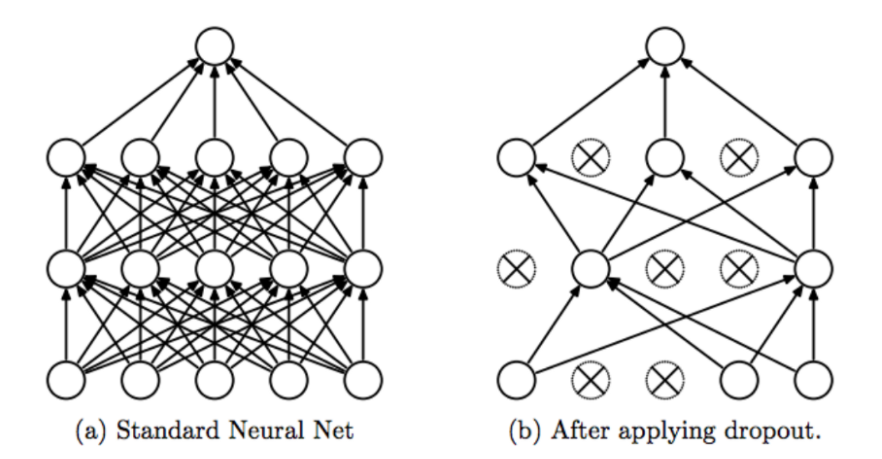
\includegraphics[width=0.7\textwidth]{figure3}
    \caption{Mô hình trước và sau khi áp dụng dropout. Nguồn ảnh: \cite{JMLR:v15:srivastava14a}.}
\end{figure}

\section{Các nghiên cứu có liên quan}

Chuyển chế độ màu ảnh nội soi thuộc vào lớp bài toán Image Translation - chuyển đổi từ dữ liệu ảnh này sang dữ liệu ảnh khác thỏa mãn yêu cầu nhất định. Với khả năng tự động học cách sinh dữ liệu thực tế, GAN trở thành một hướng tiếp cận hiển nhiên để xử lý các bài toán dạng này.

Dưới đây điểm qua ưu điểm và nhược điểm của một số nghiên cứu về sử dụng GAN vào việc giải bài toán Image Translation, qua đó giải thích lý do lựa chọn mô hình StarGAN v2 cho đồ án tốt nghiệp này.

\subsection{Pix2pix}

\begin{figure}[H]
    \centering
    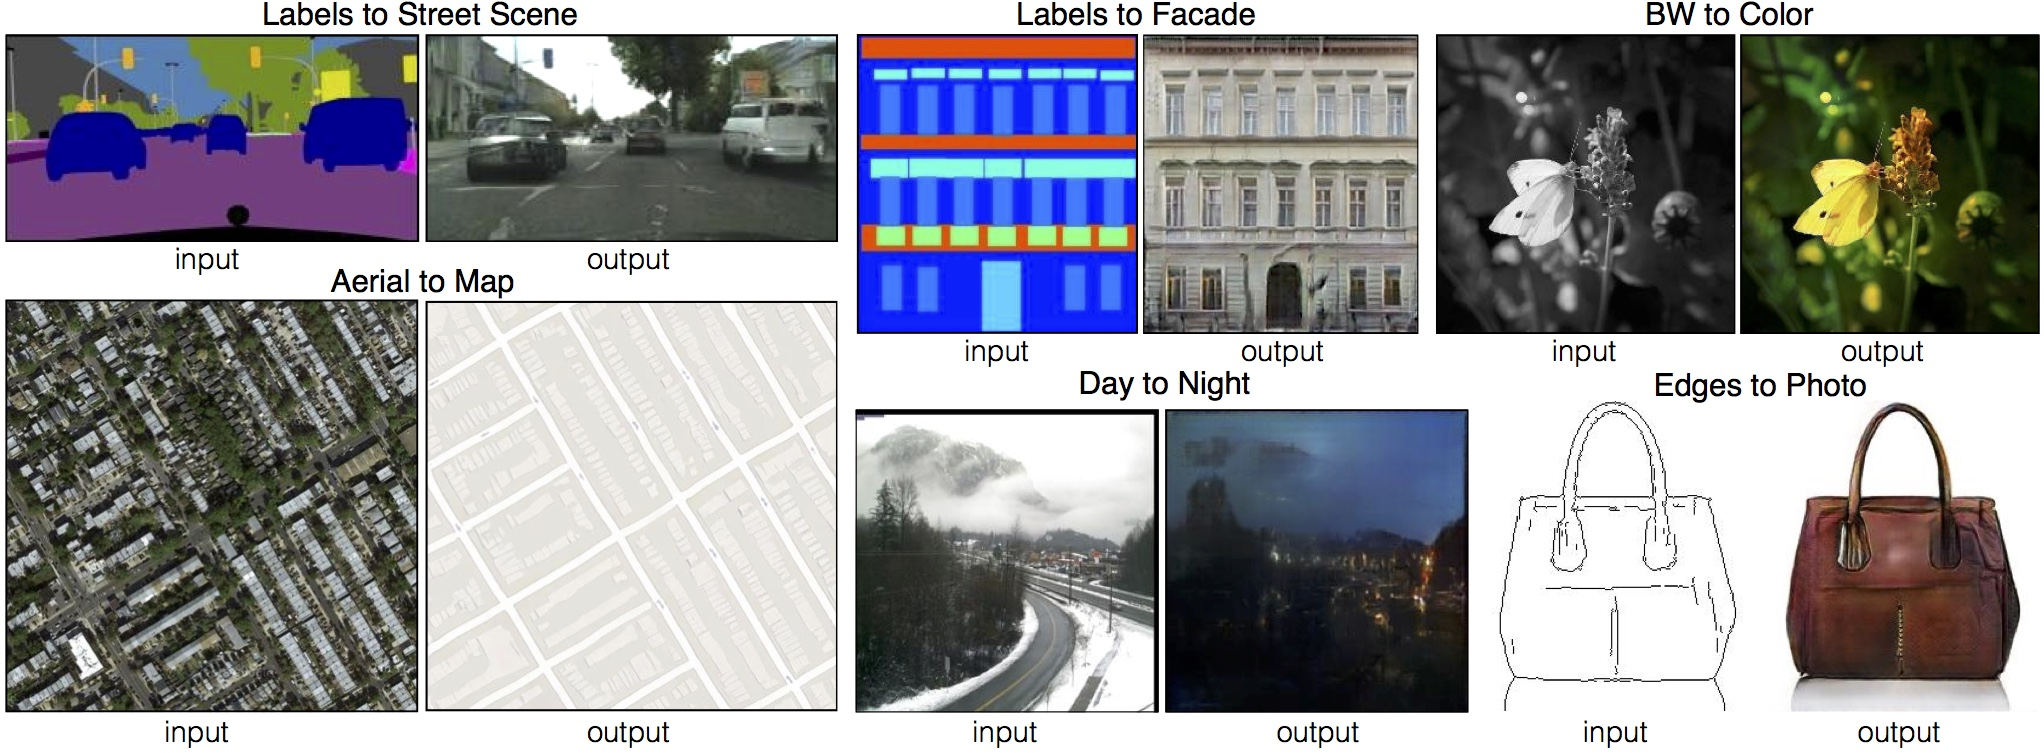
\includegraphics[width=\textwidth]{figure14}
    \caption{Một số ứng dụng của Pix2pix. Nguồn ảnh: \cite{pix2pix2017}.}
\end{figure}

Pix2pix được phát triển bởi và công bố vào năm 2017 bởi các nhà nghiên cứu của trường Đại học California \cite{pix2pix2017}. Khác với mô hình GAN cổ điển, Pix2pix không sử dụng vector latent làm đầu vào cho generator, thay vào đó sử dụng ảnh gốc. Generator sử dụng ảnh gốc để xây dựng ảnh mới có kích cỡ tương tự - giải thích tên gọi Pixel to Pixel - trong khi discriminator giữ nguyên chức năng phân loại ảnh thật/giả.

Tư tưởng của Pix2pix rất đơn giản, song mô hình này có thể hoạt động hiệu quả trên nhiều bài toán Image Translation như tự động hoàn thành ảnh dựa trên nét vẽ, tô màu ảnh đen trắng, phân vùng các đối tượng trong ảnh\dots Tuy nhiên, nhược điểm của mô hình này là yêu cầu cần phải có dữ liệu hình ảnh được gắn nhãn thành cặp trước và sau biến đổi. Trong trong phần lớn trường hợp, bao gồm bài toán đổi màu ảnh nội soi, việc xây dựng bộ dữ liệu theo cặp là rất khó khăn, thậm chí không thể thực hiện được.

\subsection{CycleGAN}

Cũng trong năm 2017, nhóm nghiên cứu của trường Đại học California đề xuất mô hình sinh ảnh CycleGAN, khắc phục được yêu cầu dữ liệu ảnh theo cặp của Pix2pix.

\begin{figure}[H]
    \centering
    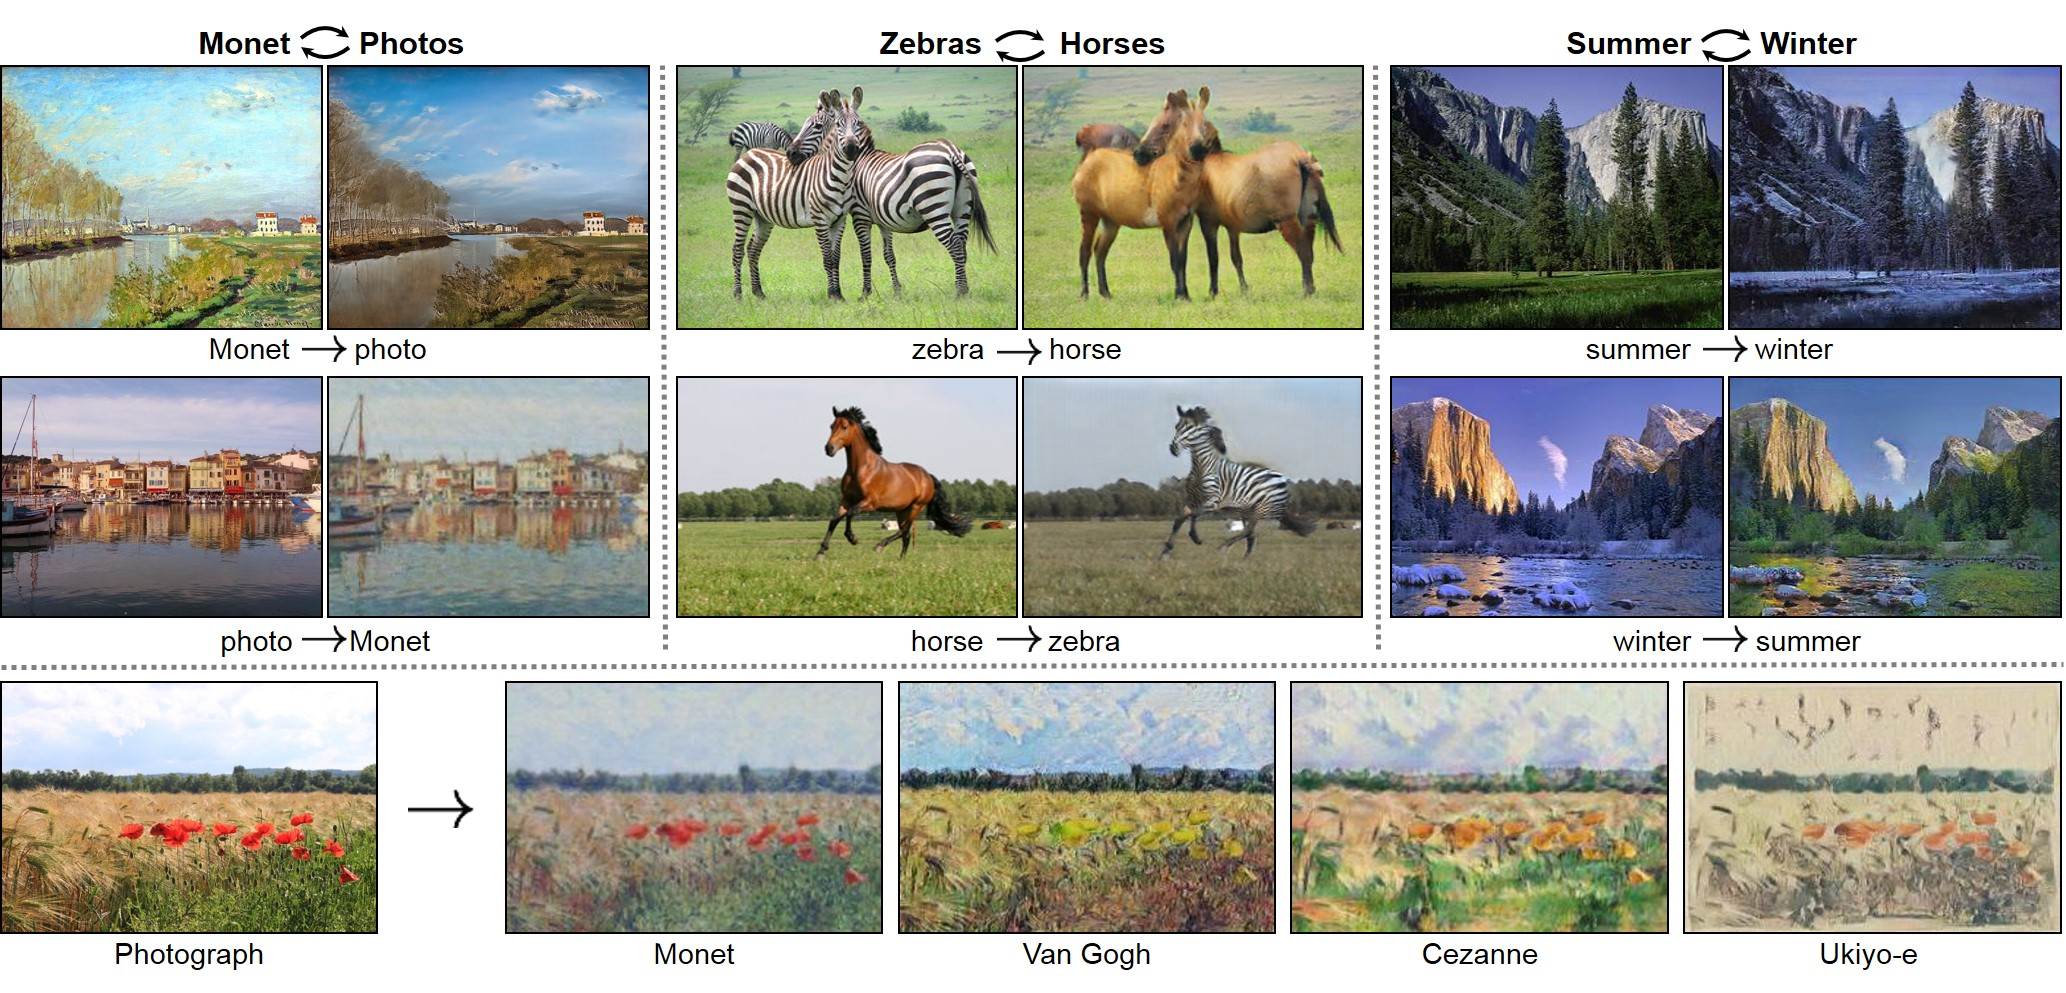
\includegraphics[width=\textwidth]{figure15}
    \caption{Một số ứng dụng của CycleGAN. Nguồn ảnh: \cite{CycleGAN2017}.}
\end{figure}

CycleGAN lấy cảm hứng từ các mô hình autoencoder - mạng nén dữ liệu với số chiều cao thành vector latent có số chiều thấp. Mô hình autoencoder được đánh giá là tốt nếu như quá trình nén đảm bảo toàn vẹn dữ liệu. Tương tự, kiến trúc CycleGAN ngoài hai generator $ G_A $ và discriminator $ D_A $ giống như Pix2pix, còn sử dụng thêm một generator $ G_B $ để biến đổi đầu ra của $ G_B $ về ảnh đầu vào gốc, cùng với một discriminator $ D_B $ để phân loại thật/giả kết quả của $ G_B $. Bằng việc tối ưu cả 4 mô hình, ta kì vọng $ G_A $ và $ G_B $ có thể học được cách biến đổi ảnh đầu vào thành ảnh mục tiêu thỏa mãn, đồng thời vẫn giữ lại được đủ thông tin cần thiết để xây dựng lại ảnh ban đầu.

Khi luyện tập CycleGAN, ta sử dụng hàm mục tiêu minimax cổ điển trên cả 4 mạng:
\begin{align*}
    L_{adv} = & E_{y \in Y} [\log(D_A(y))] + E_{x \in X} [\log(1 - D_A(G_A(x)))] \\
    +         & E_{x \in X} [\log(D_B(x))] + E_{y \in Y} [\log(1 - D_B(G_B(y)))]
\end{align*}
cùng với một hàm mục tiêu mới cycle consistency, thể hiện sự khác biệt giữa ảnh thật và ảnh khôi phục:
\begin{align*}
    L_{cyc} = & E_{x \in X} [|G_B(G_A(x)) - x|] + E_{y \in Y} [|G_A(G_B(y)) - y|]
\end{align*}

Hàm mục tiêu đầy đủ của CycleGAN có công thức:
$$ L = L_{adv} + \lambda_{cyc} L_{cyc} $$
với $ \lambda_{cyc} $ là hệ số do người dùng lựa chọn.

\begin{figure}[H]
    \centering
    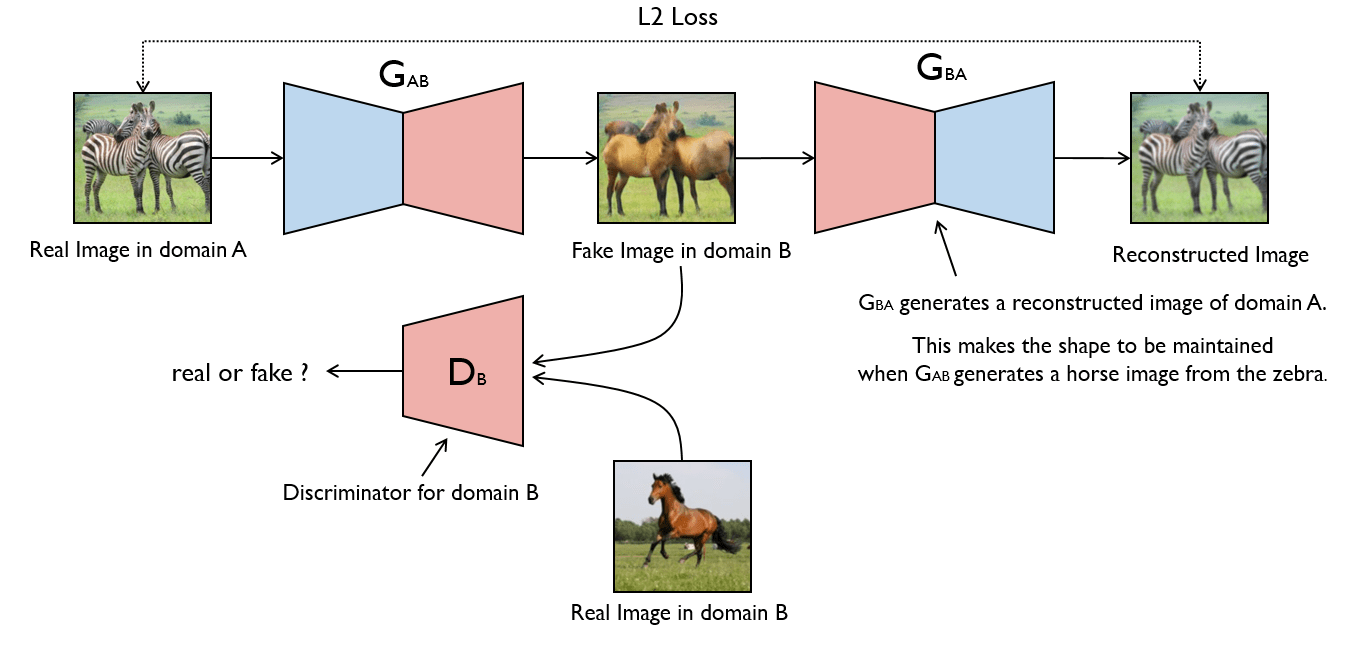
\includegraphics[width=\textwidth]{figure16}
    \caption{Kiến trúc các mạng và hai hàm mục tiêu của CycleGAN. Nguồn ảnh: \cite{mnistsvhntransfer}.}
\end{figure}

Ưu điểm của CycleGAN là loại bỏ rào cản về dữ liệu luyện tập - nhóm nghiên cứu liệt kê ra một loạt các bài toán mà các phương án trước CycleGAN không thể giải quyết được, bao gồm chuyển đổi phong cách ảnh, chuyển đổi đối tượng trong ảnh mà vẫn giữ nguyên tư thế, chuyển đổi mùa của ảnh chụp phong cách, sinh ảnh thực tế từ tranh vẽ,\dots Tuy nhiên, một generator của CycleGAN chỉ có thể chuyển đổi ảnh từ một lớp sang một lớp khác. Để áp dụng vào bài toán chuyển đổi 4 chế độ màu của đồ án này, ta cần luyện tập 12 mô hình - rất tốn thời gian và tài nguyên tính toán.

\subsection{StarGAN (v1)}

\begin{figure}[H]
    \centering
    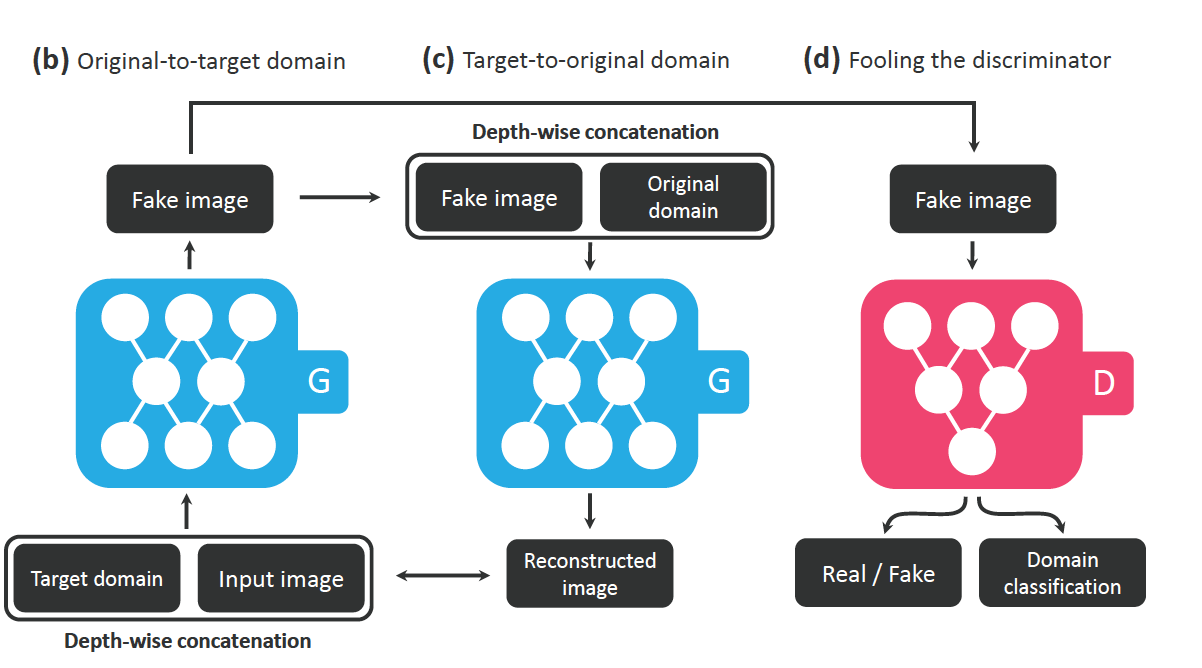
\includegraphics[width=0.8\textwidth]{figure17}
    \caption{Kiến trúc các mạng và hai hàm mục tiêu của StarGAN v1. Nguồn ảnh: \cite{DBLP:journals/corr/abs-1711-09020}.}
\end{figure}

Phiên bản đầu tiên của StarGAN được công bố vào năm 2017 bởi nhóm nghiên cứu Clova AI, trực thuộc tập đoàn NAVER \cite{DBLP:journals/corr/abs-1711-09020}. StarGAN có thể làm việc với nhiều lớp dữ liệu ảnh cùng một lúc chỉ với một mạng generator duy nhất, qua đó giải quyết được vấn đề mở rộng của CycleGAN.

Kiến trúc của StarGAN v1 gần giống với kiến trúc của CycleGAN, với một số thay đổi sau:
\begin{itemize}
    \item Mô hình không có generator và discriminator riêng cho từng lớp một, thay vào đó sử dụng chung một generator $ G $ và một discriminator $ D $.
    \item Generator nhận vào ảnh gốc, cùng với chỉ số của lớp ảnh mục tiêu và cho ra ảnh đã được biến đổi thuộc lớp đó.
    \item Discriminator cho ra dự đoán ảnh thật/giả, đồng thời cũng phân loại ảnh vào một trong các lớp.
\end{itemize}

StarGAN cũng sử dụng hàm mục tiêu minimax và hàm cycle consistency, tuy nhiên hàm minimax được sửa lại để tương tích với bài toán phân loại ảnh nhiều lớp.

Bài báo gốc đánh giá StarGAN bằng cách khảo sát ý kiến người thật khi so sánh với các hình ảnh sinh ra bởi CycleGAN, DIAT và IcGAN. Kết quả khảo sát cho thấy StarGAN cho ra hình ảnh với độ sắc nét cao, chất lượng vượt trội hơn tất cả các mô hình còn lại. Điều này có được là nhờ ưu thế dữ liệu của StarGAN - do các mô hình còn lại chỉ được huấn luyện với từng cặp 2 lớp, generator không học được nhiều đặc điểm chung giữa tất cả các lớp. StarGAN được tiếp xúc với dữ liệu của tất cả các lớp, vì thế có thể học được kiến thức này một cách dễ dàng.

Phiên bản StarGAN được sử dụng trong báo cáo là StarGAN v2, được công bố bởi Clova AI vào năm 2019 \cite{DBLP:journals/corr/abs-1912-01865}. Phiên bản cải tiến này nhắm tới việc đa dạng hóa khả năng sinh ảnh của mô hình StarGAN gốc - với một cặp ảnh gốc và lớp ảnh mục tiêu, StarGAN v2 cho phép sinh ra vô số ảnh khác nhau thỏa mãn điều kiện.

\section{Các chế độ màu}

Để hiểu rõ hơn về bài toán chuyển đổi chế độ màu, ta cần điểm qua đặc điểm của từng chế độ, qua đó rút ra yêu cầu mà mô hình thành quả cần đạt được.

\subsection{Blue Light Imagining (BLI)}

BLI thừa hưởng cơ chế hoạt động của Narrow Band Imagining (NBI) - một kĩ thuật IEE đời đầu. NBI sử dụng hai chùm tia sáng xanh dương (bước sóng 415 $ \pm $ 30 nm) và xanh lục (bước sóng 540 $ \pm $ 30 nm) để tăng cường chất lượng ảnh. Do huyết sắc tố hấp thụ mạnh các bước ánh sáng này, mạch máu sẽ trở nên đậm màu hơn so với các niêm mạc xung quanh, giúp cho việc nhận dạng các tổn thương trở nên dễ dàng hơn.

Khác với NBI, BLI sử dụng hai đèn laser ở bước sóng 410 $ \pm $ 10 nm và 450 $ \pm $ 10 nm thay cho đèn xenon của NBI. Ngoài tác dụng làm nổi mạch máu, laser 450 nm cũng có tác dụng kích thích phosphor ở đầu ống nội soi để cung cấp ánh sáng trắng. Bằng cách điều chỉnh cường độ của hai đèn laser, bác sĩ có thể lựa chọn giữa quan sát tổng quát các mạch máu ở xa và sâu, hoặc ưu tiên quan sát kĩ các tổn thương ở bề mặt \cite{pmid26770267}.

Do được chiếu sáng bằng hai đèn xanh dương và xanh lục, ảnh nội soi sử dụng BLI thường có màu trắng - xám, ít sắc đỏ. Mạch máu có màu sắc tương phản rõ ràng so với niêm mạc xung quanh.

\begin{figure}[H]
    \centering
    \begin{subfigure}[H]{0.45\textwidth}
        \centering
        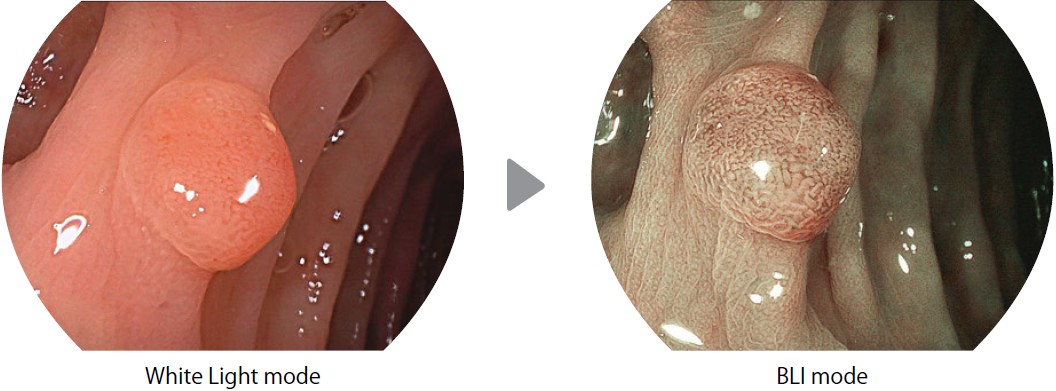
\includegraphics[width=\linewidth]{figure19.jpg}
        \caption{WLI}
    \end{subfigure}
    \begin{subfigure}[H]{0.45\textwidth}
        \centering
        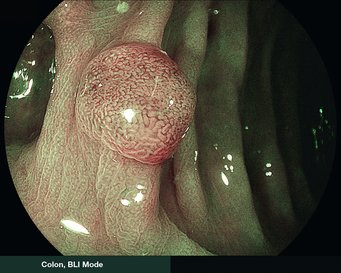
\includegraphics[width=\linewidth]{figure18.jpg}
        \caption{BLI}
    \end{subfigure}
    \caption{So sánh ảnh nội soi WLI và BLI tại cùng một vị trí. Nguồn ảnh: Fujifilm.}
\end{figure}

\subsection{Flexible spectral Imagining Color Enhancement - (FICE)}

Khác với BLI là kĩ thuật tiền xử lý ảnh nội soi (thay đổi môi trường ánh sáng trước khi camera ghi nhận), FICE là kĩ thuật hậu xử lý, tăng cường chất lượng ảnh nội soi trong bước tổng hợp dữ liệu sau khi camera ghi nhận.

\begin{figure}[H]
    \centering
    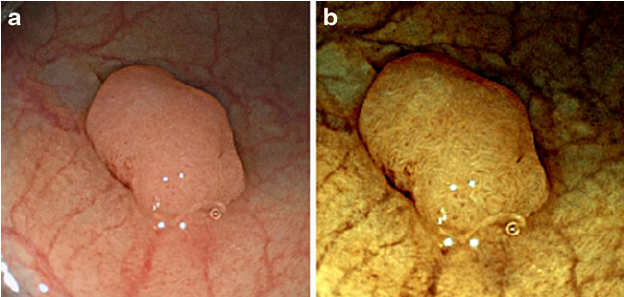
\includegraphics[width=0.9\linewidth]{figure20.png}
    \caption{So sánh ảnh nội soi (a) WLI và (b) FICE tại cùng một vị trí. Nguồn ảnh: \cite{s0038401113808}}
\end{figure}

FICE tăng cường các dải tần ánh sáng đặc biệt trước khi tổng hợp thành ảnh cuối cùng. Các dải tần này có thể là dải ánh sáng bị hấp thụ bởi mạch máu (từ 400 tới 420 nm), bị phản xạ bởi mạch máu (khoảng 470 nm), bị phản xạ bởi niêm mạc (khoảng 500 nm) hoặc bị hấp thụ bởi huyết sắc tố (khoảng 550 nm). Lựa chọn dải tần phù hợp giúp tăng cường độ tương phản giữa các đối tượng trong ảnh nội soi. Tuy nhiên, ảnh FICE bị ám màu vàng không tự nhiên và thường bị tối.

\subsection{Linked Color Imagining (LCI)}
\label{lci}

LCI sử dụng cả kĩ thuật tiền xử lý như NBI và BLI và hậu xử lý như FICE để tăng cường chất lượng hình ảnh. Ảnh nội soi sử dụng LCI không chỉ có độ tương phản giữa các đối tượng cao, được rọi sáng rõ ràng mà còn có khả năng làm nổi bật các tổn thương do ung thư bằng màu sắc.

\begin{figure}[H]
    \centering
    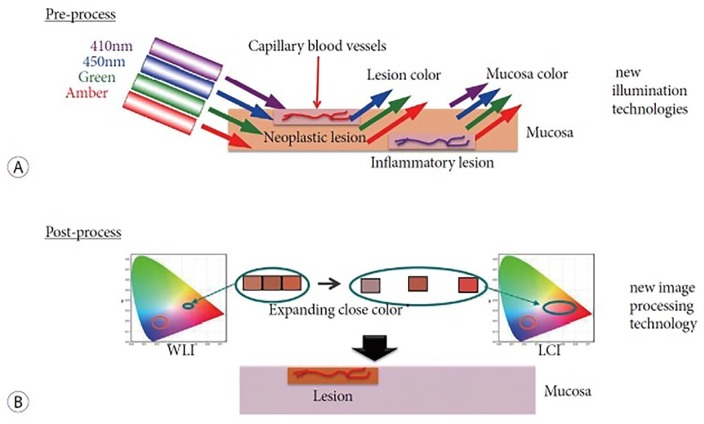
\includegraphics[width=0.9\linewidth]{figure21.jpg}
    \caption{Hai bước xử lý của LCI. (a) Tiền xử lý với một số tần số ánh sáng nhất định. Ánh sáng tím bị hấp thụ bởi các khối u ung thư, nhưng không bị hấp thụ bởi niêm mạc bị viêm. (b) Các màu sắc gần giống nhau được tăng độ tương phản. Nguồn ảnh: \cite{pmid31700545}}
\end{figure}

Trong bước tiền xử lý, LCI sử dụng 4 nguồn sáng tím (410 nm), xanh dương (450 nm), xanh lá và đỏ. Ánh sáng tím dễ bị hấp thụ bởi các mao mạch nông của khối u ung thư, khiến cho các khối u này có màu đỏ-cam khi lên ảnh. Ngược lại, niêm mạc bình thường không có mao mạch nông, do đó ánh sáng tím không bị hấp thụ, bề mặt niêm mạc lên ảnh có màu ám tím.

Trong bước hậu xử lý, các màu sắc thực tế của ảnh được giãn cách xa nhau để tăng cường độ tương phản.

LCI là chế độ màu khó tái tạo lại nhất trong cả 4 chế độ. Trong khi BLI, FICE và WLI chỉ khác nhau về màu sắc và độ tương phản của các đối tượng, LCI còn có thêm khả năng phát hiện mô ung thư. Ngoại việc rút ra tri thức về màu sắc của các lớp ảnh, mô hình học máy còn cần phải hiểu được thông tin nội dung của ảnh để có thể thay đổi màu khối u cho phù hợp.

\subsection{White Light Imagining (WLI)}

Đây là chế độ ảnh nội soi với đèn trắng cơ bản, không có tính năng gì đặc biệt.

\chapter{Phương pháp đề xuất}

Để giải quyết bài toán chuyển đổi chế độ màu ảnh y tế, đồ án này sử dụng mô hình học sâu StarGAN v2, được công bố bởi nhóm nghiên cứu Clova AI vào năm 2019. Chương này đi sâu vào giải thích tư tưởng của nghiên cứu gốc, những thay đổi để phù hợp với yêu cầu của đề tài, kiến trúc cụ thể của các mạng và các hàm mục tiêu được sử dụng.

\section{Tư tưởng thiết kế}

StarGAN v2 là bản cập nhật của mô hình StarGAN năm 2017, bổ sung thêm khả năng đa dạng hóa kết quả: với cùng một lớp mục tiêu, StarGAN v2 có thể sinh ra vô số ảnh thỏa mãn có phong cách khác nhau.

\begin{figure}[H]
    \centering
    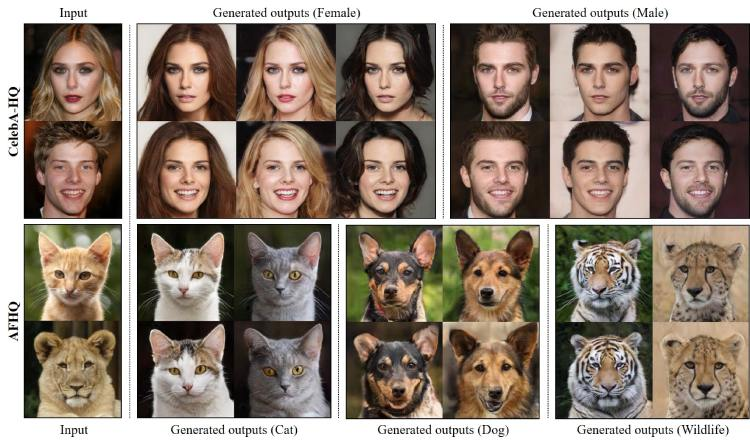
\includegraphics[width=\linewidth]{figure22.jpg}
    \caption{Một số ví dụ về kết quả sinh ảnh của StarGAN v2 trên bộ ảnh người nổi tiếng (CelebA-HQ) và bộ ảnh động vật (AFHQ). Nguồn ảnh: \cite{choi2020stargan}}
\end{figure}

Thay vì chỉ định lớp ảnh mục tiêu cụ thể, StarGAN v2 sử dụng vector mô tả phong cách. Với ảnh đầu vào $ x $ và vector phong cách $ s $ thuộc lớp $ y $, generator $ G $ cần phải học được cách sinh ảnh mới $ x' $ theo phong cách được chỉ định, nhằm đánh lừa discriminator $ D $ phân loại $ x' $ về đúng lớp mục tiêu $ y $.

Để sinh ra vector phong cách, StarGAN v2 bổ sung thêm hai mạng học sâu:
\begin{enumerate}
    \item Style encoder $ E $: Nhận vào ảnh thật $ x $ cùng với lớp của ảnh $ y $, trả về vector $ s $ mã hóa phong cách của $ x $ theo $ y $.
    \item Mapping network $ F $: Nhận vào vector latent $ z $ cùng với lớp $ y $, trả về vector phong cách ảnh $ s $ thuộc về lớp $ y $.
\end{enumerate}
Khi sinh ảnh mới, ta có thể kết hợp generator với style encoder để sinh ảnh với phong cách của ảnh đối chiếu, hoặc kết hợp với mapping network để sinh ảnh với phong cách ngẫu nhiên. Trong cài đặt thực tế, khi chuyển đổi ảnh thật sang ảnh thuộc một lớp khác, ta thường sử dụng vector phong cách trung bình của lớp mục tiêu, được tính bằng cách đưa một lượng lớn ảnh thật vào Style Encoder hoặc đưa một lượng lớn vector latent ngẫu nhiên vào Mapping Network:
$$ E_y[s] \approx \cfrac{1}{N} \sum_{i = 1}^{n} E(x_{y, i}, y) \approx \cfrac{1}{N} \sum_{i = 1}^{n} F(z_{i}, y) $$

\begin{figure}[H]
    \centering
    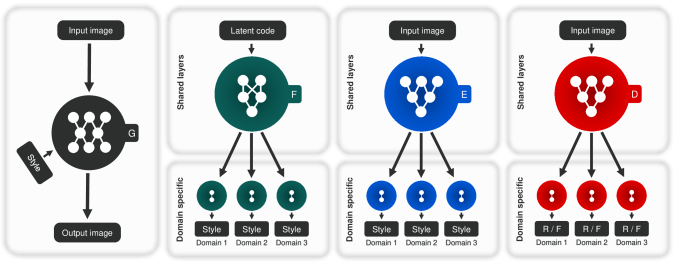
\includegraphics[width=\linewidth]{figure23.png}
    \caption{Kiến trúc mạng của StarGAN v2. Từ trái qua: generator, mapping network, style encoder và discriminator. Nguồn ảnh: \cite{choi2020stargan}}
\end{figure}

Khả năng biểu diễn phong cách của ảnh dưới dạng vector cũng cho phép mạng StarGAN v2 điều khiển mức độ chuyển đổi ảnh: với $ s_{x} $ là vector phong cách của ảnh gốc, $ s' $ là vector phong cách mục tiêu, ta có thể chuyển đổi ảnh một phần tới vector phong cách:
$$ s_{\psi} = \psi s' + (1 - \psi) s_{x} $$
với $ \psi \in [0, 1] $, tương ứng với mức độ từ hoàn toàn giữ nguyên tới hoàn toàn chuyển đổi.

\begin{figure}[H]
    \centering
    \begin{subfigure}[H]{0.19\textwidth}
        \centering
        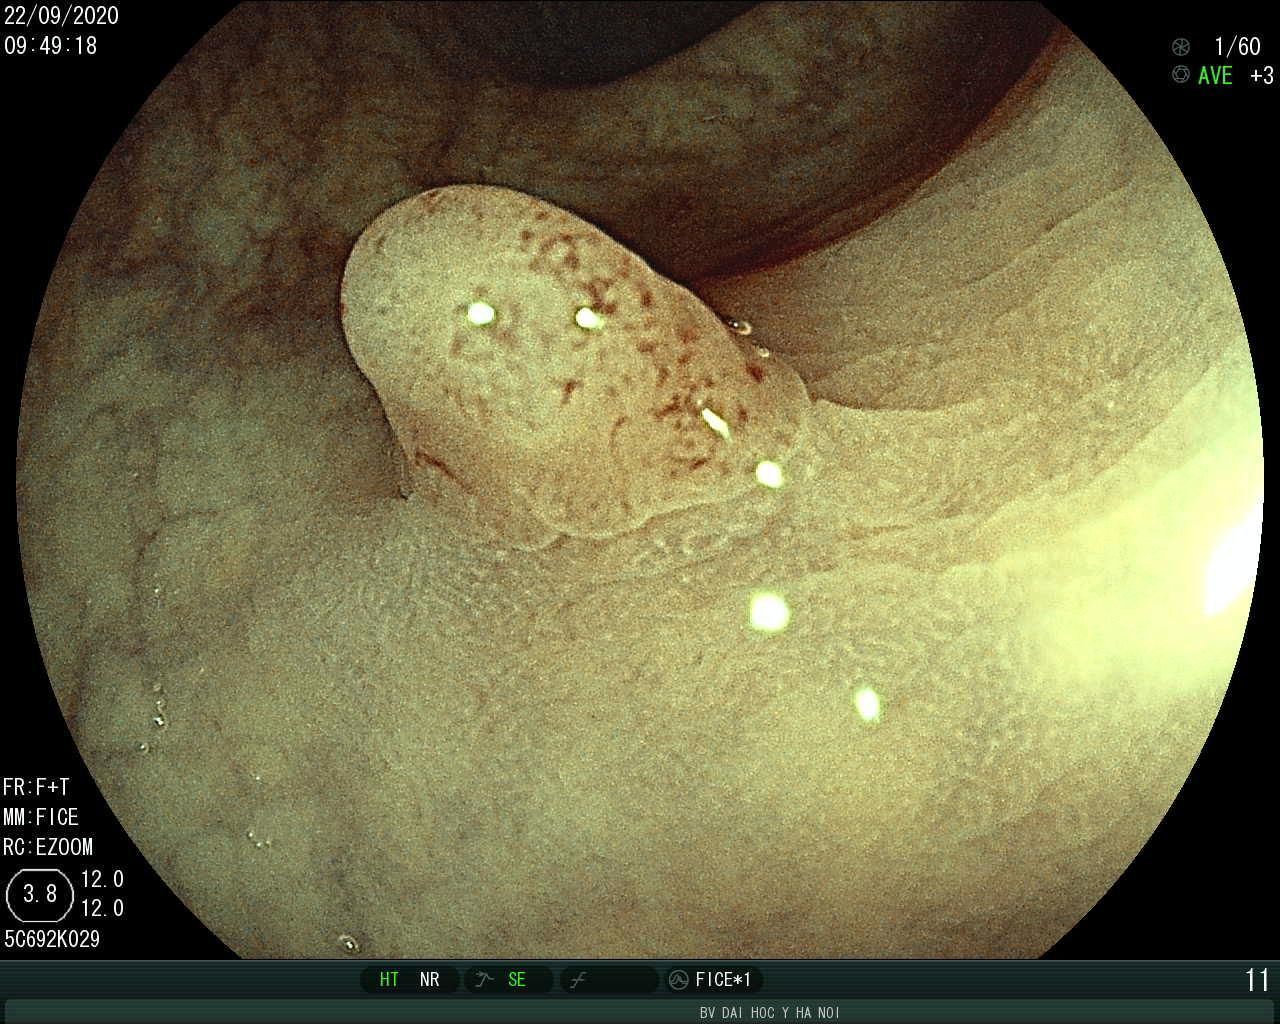
\includegraphics[width=\linewidth]{psi/0c56215fcd9b61e15625e0984adce794.jpeg}
        \caption{Ảnh gốc}
    \end{subfigure}
    \begin{subfigure}[H]{0.19\textwidth}
        \centering
        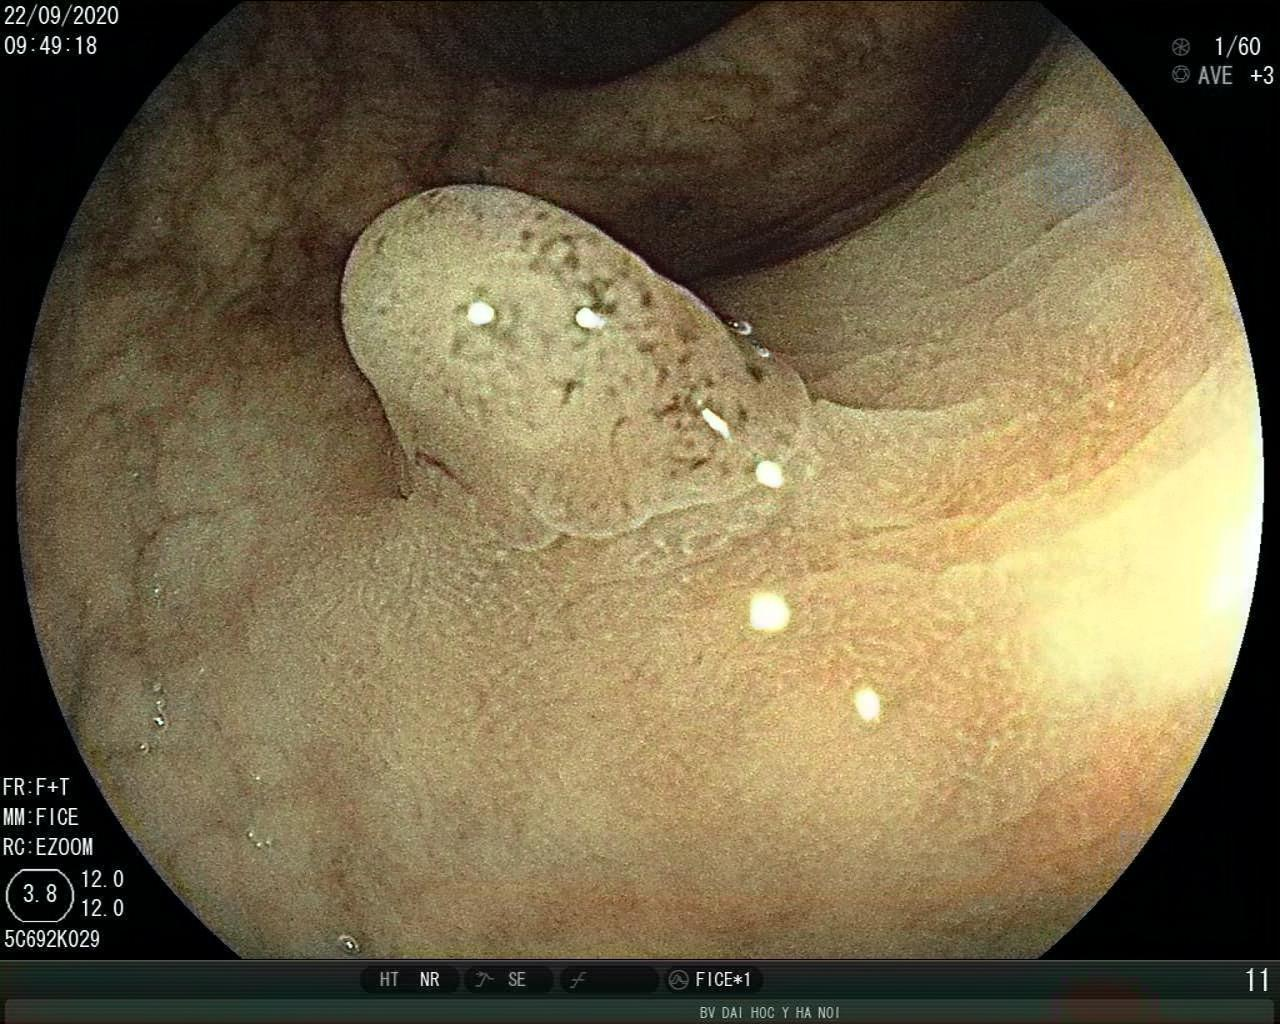
\includegraphics[width=\linewidth]{psi/03.jpeg}
        \caption{$ \psi = 0.3 $}
    \end{subfigure}
    \begin{subfigure}[H]{0.19\textwidth}
        \centering
        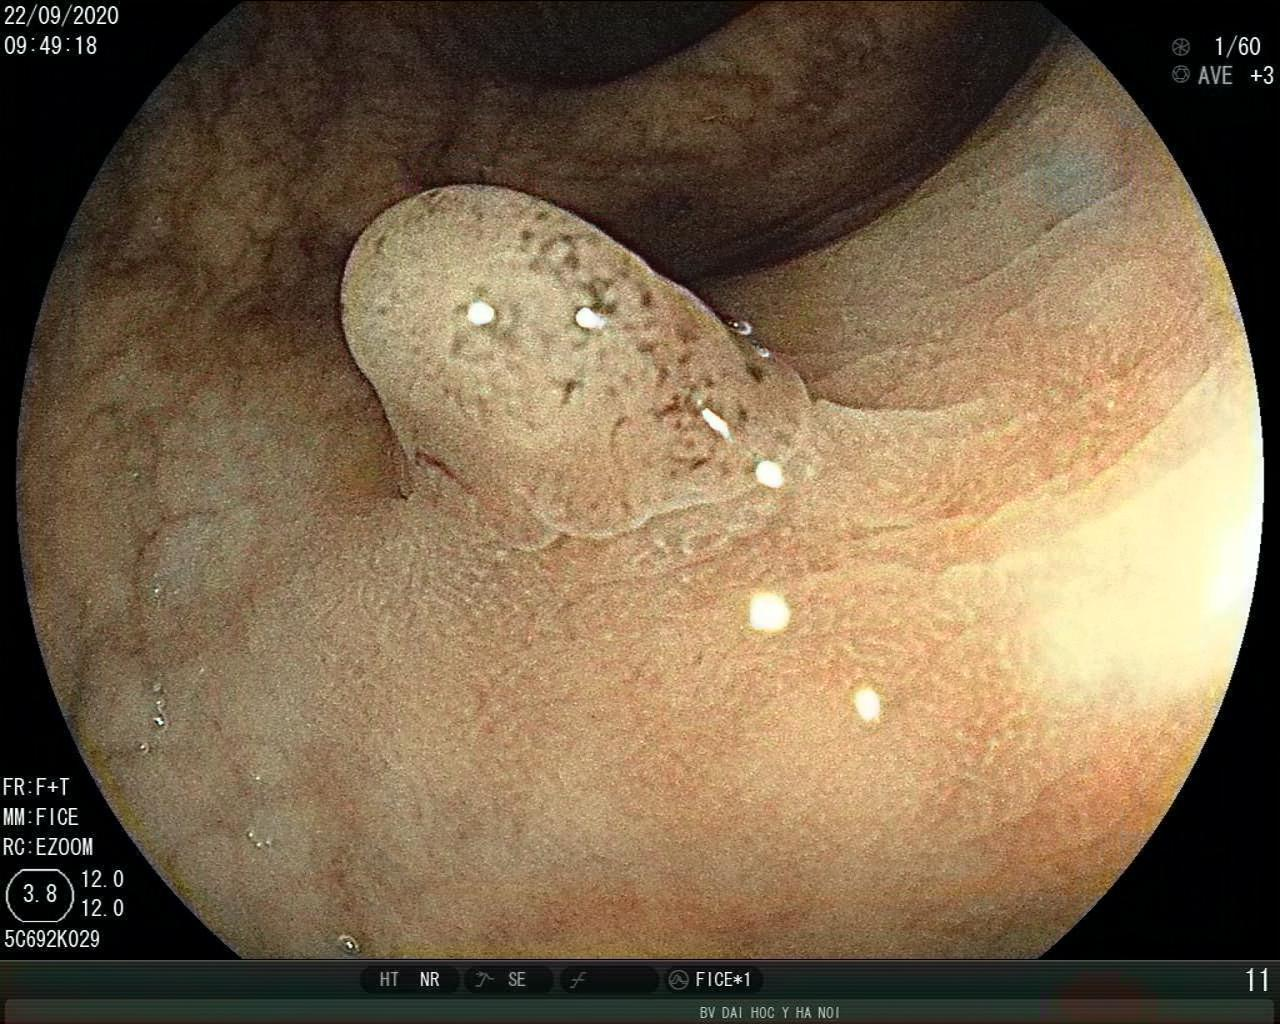
\includegraphics[width=\linewidth]{psi/05.jpeg}
        \caption{$ \psi = 0.5 $}
    \end{subfigure}
    \begin{subfigure}[H]{0.19\textwidth}
        \centering
        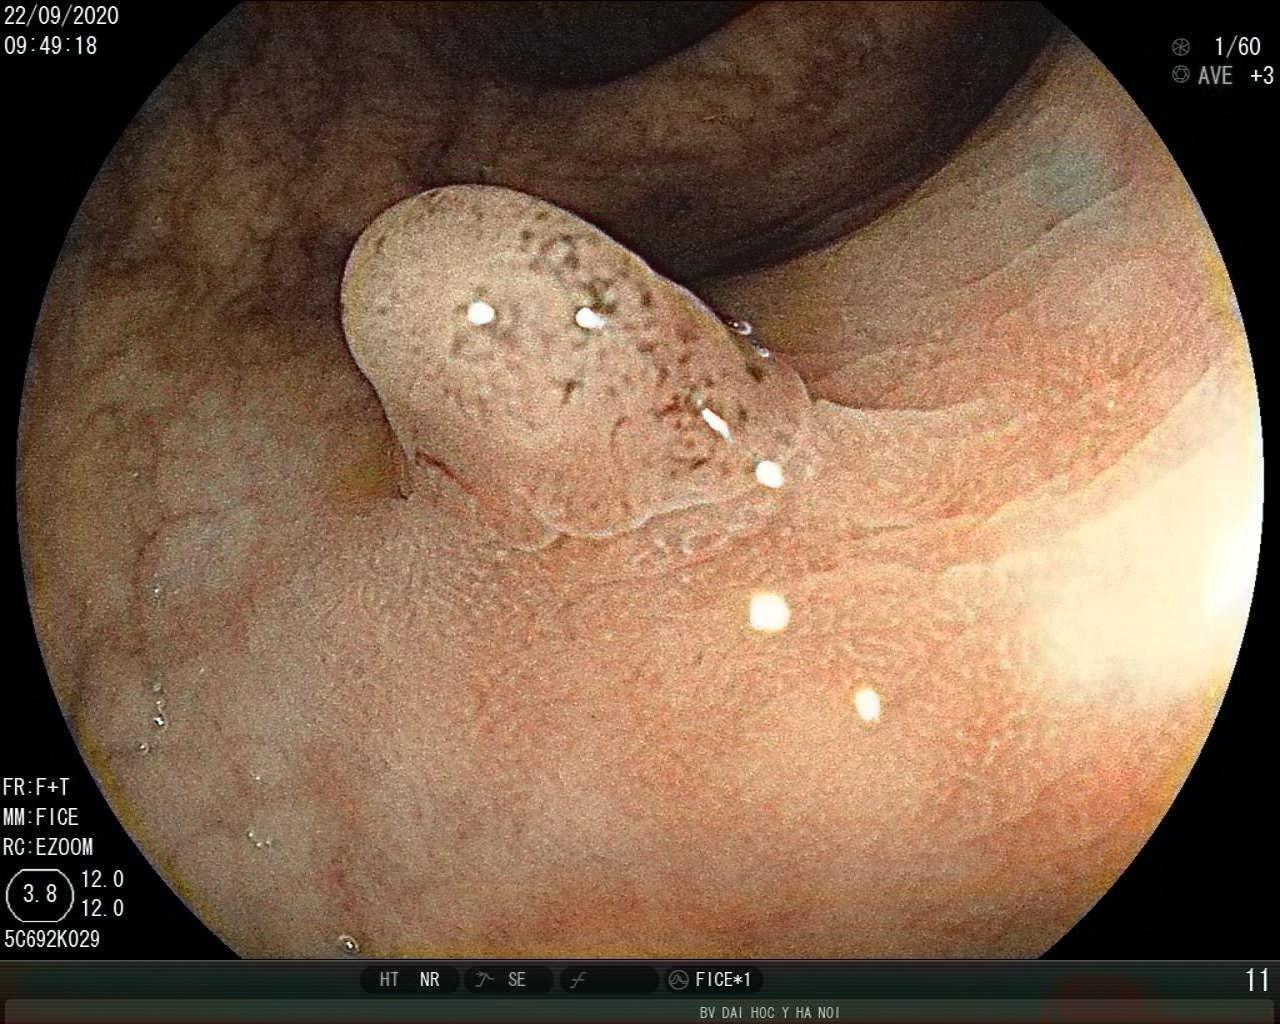
\includegraphics[width=\linewidth]{psi/07.jpeg}
        \caption{$ \psi = 0.7 $}
    \end{subfigure}
    \begin{subfigure}[H]{0.19\textwidth}
        \centering
        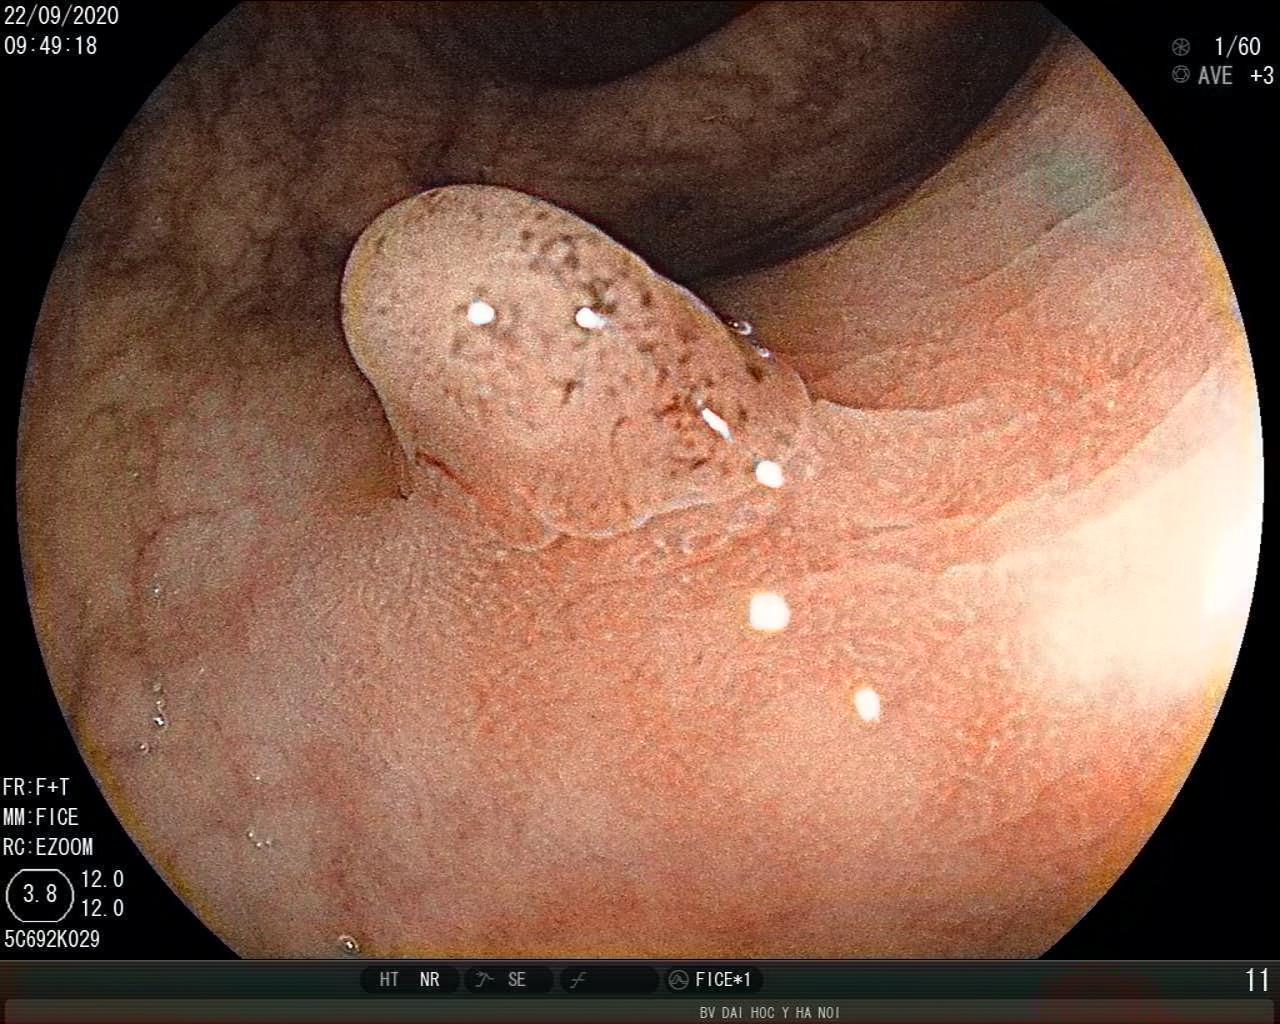
\includegraphics[width=\linewidth]{psi/1.jpeg}
        \caption{$ \psi = 1 $}
    \end{subfigure}
    \caption{Chuyển đổi ảnh FICE sang WLI một phần sử dụng StarGAN v2.}
\end{figure}

Trong nghiên cứu gốc, nhóm tác giả so sánh StarGAN v2 với ba mô hình sinh ảnh khác là MUNIT, DRIT và MSGAN trên hai bộ dữ liệu ảnh người nổi tiếng (CelebA-HQ) và ảnh động vật (AFHQ). Kết quả đánh giá định lượng (sử dụng hai chỉ số FID và LPIPS) và định tính (sử dụng đánh giá của người thực) cho thấy StarGAN v2 sinh ra ảnh chất lượng cao hơn cả ba mô hình còn lại. Nhóm tác giả đưa ra ba lý do giải thích sự vượt trội của StarGAN v2:
\begin{itemize}
    \item Thứ nhất, generator của StarGAN v2 chỉ cần tập trung vào việc sử dụng vector phong cách, trong khi tất các các thông tin liên quan tới lớp ảnh mục tiêu đã được xử lý bởi hai mạng style encoder và mapping network.
    \item Thứ hai, vì vector phong cách của StarGAN v2 được sinh ra bởi mạng học sâu, phân bố xác suất của các vector này phức tạp hơn so với các mô hình sinh ảnh sử dụng vector latent lấy ngẫu nhiên.
    \item Cuối cùng, StarGAN v2 thừa hưởng lợi thế về dữ liệu luyện tập của phiên bản 1: nhờ việc có thể tiếp cận với tất cả các ảnh của tất cả các lớp, StarGAN v2 học được nhiều thuộc tính chung giữa các lớp hơn, qua đó cải thiện khả năng khái quát hóa của mô hình.
\end{itemize}

\section{Thay đổi so với nghiên cứu gốc}

Nhóm nghiên cứu Clova AI đưa ra ví dụ về việc sinh ảnh mới của người và động vật, sao cho tư thế của ảnh gốc được giữ nguyên. So với ví dụ của bài báo gốc, bài toán đổi chế độ màu của ảnh nội soi có hai điểm khác biệt:
\begin{itemize}
    \item Ta chỉ muốn thay đổi màu sắc, độ sáng và độ tương phản của ảnh gốc, tuyệt đối không để nội dung của ảnh gốc bị ảnh hưởng. Để giải quyết vấn đề này, ta thực hiện tính toán trên không gian màu YCbCr.
    \item Để phân loại ảnh người và động vật, discriminator cần sử dụng thông tin của toàn bộ ảnh. Ngược lại, ta không cần nhìn toàn bộ ảnh nội soi để biết chế độ màu - chỉ cần nhìn một vùng nhỏ là có thể phân loại được. Mô hình trong đồ án sử dụng kiến trúc discriminator PatchGAN để lợi dụng đặc điểm này.
\end{itemize}

\subsection{Không gian màu YCbCr}
\label{ycbcr-colorspace}

Giống như CycleGAN và StarGAN phiên bản 1, generator của StarGAN v2 lấy cảm hứng từ mạng autoencoder: ảnh nguyên bản được đưa qua qua một loạt các lớp convolutional để nén thành dữ liệu nén có kích thước nhỏ, sau đó đi qua một loạt các lớp convolutional để giải nén thành ảnh đầu ra. Quá trình nén dữ liệu từ không gian nhiều chiều xuống không gian ít chiều hơn dù có tốt tới đâu cũng không tránh khỏi mất mát thông tin, khiến cho ảnh đầu ra không thể giống hệt ảnh đầu vào. Sai số này không phải là vấn đề lớn đối với bài toán sinh ảnh người và vật, song lại là không thể chấp nhận được đối với các lĩnh vực cần độ chính xác cao như chẩn đoán nội soi.

Để giải quyết vấn đề này, thay vì để generator chịu trách nhiệm sinh toàn bộ ảnh, ta chỉ yêu cầu generator sinh ra phong cách, rồi kết hợp phong cách này cùng với bố cục gốc để cho ra ảnh mới. Để bảo toàn bố cục gốc, ta có thể sử dụng không gian màu YCbCr.

\begin{figure}[H]
    \centering
    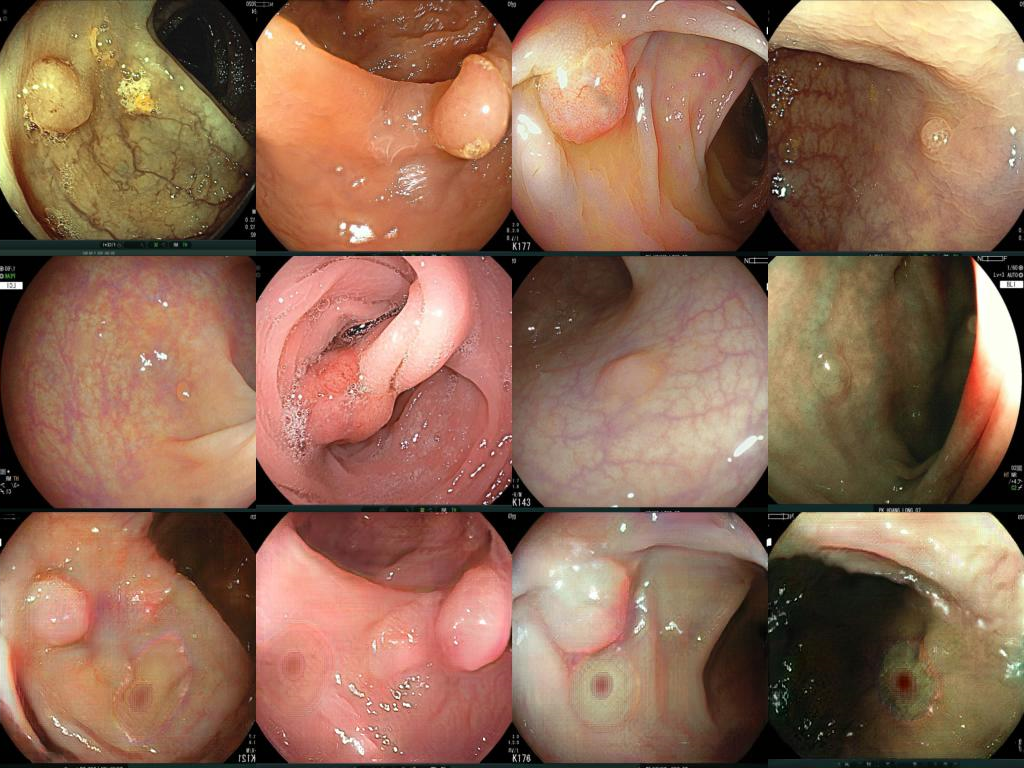
\includegraphics[width=0.9\linewidth]{figure28.png}
    \caption{Sai số khi sử dụng StarGAN v2 để biến đổi toàn bộ ảnh gốc (hàng đầu tiên) thành ảnh mới (hàng dưới cùng) sử dụng phong cách của ảnh đối chiếu (hàng giữa).}
\end{figure}

Không gian màu là các mô hình toán học mô tả màu sắc, thường dưới dạng bộ 3 hoặc bộ 4 kênh giá trị thành phần. Các thiết bị điện tử chủ yếu sử dụng không gian màu RGB, biểu diễn màu sắc dưới dạng bộ 3 số đại diện cho cường độ của ba màu đỏ - xanh lá - xanh lam. RGB có thể biểu diễn phần lớn màu sắc mà con người có thể phân biệt, rất tiện lợi cho các tác vụ đồ họa. Tuy nhiên, từ giá trị của một kênh màu đơn lẻ không thể mô tả được bố cục của ảnh.

\begin{figure}[H]
    \centering
    \begin{subfigure}[H]{\textwidth}
        \centering
        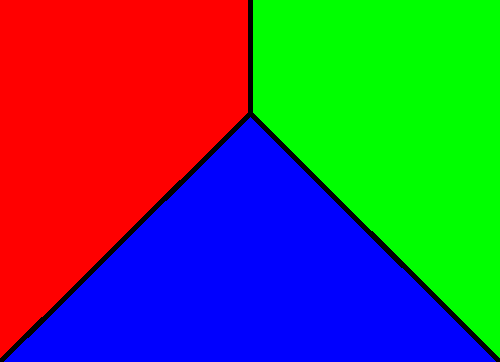
\includegraphics[width=0.3\linewidth]{figure24.png}
        \caption{Hình ảnh gốc}
    \end{subfigure}
    \begin{subfigure}[H]{0.3\textwidth}
        \centering
        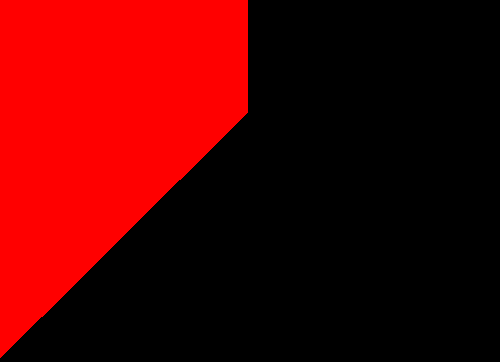
\includegraphics[width=\linewidth]{figure25.png}
        \caption{Kênh R}
    \end{subfigure}
    \begin{subfigure}[H]{0.3\textwidth}
        \centering
        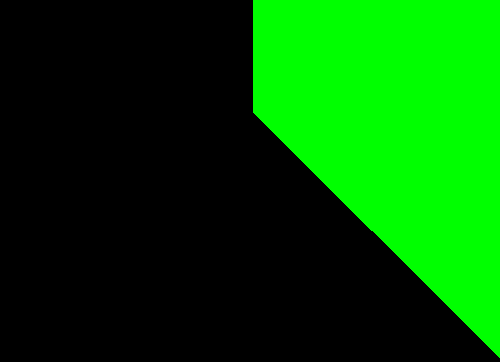
\includegraphics[width=\linewidth]{figure26.png}
        \caption{Kênh G}
    \end{subfigure}
    \begin{subfigure}[H]{0.3\textwidth}
        \centering
        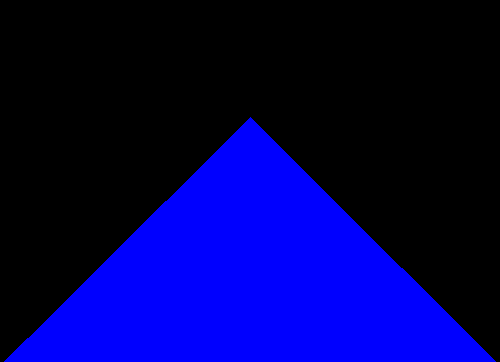
\includegraphics[width=\linewidth]{figure27.png}
        \caption{Kênh B}
    \end{subfigure}
    \caption{Biểu diễn giá trị các kênh màu của ảnh RGB.}
\end{figure}

Không gian màu YCbCr biểu diễn màu sắc bằng 3 kênh Y đại diện cho độ sáng (luma) và Cb, Cr đại diện cho cường độ màu xanh và màu đỏ (chroma) so với Y. Do mắt người nhận diện khác biệt về độ sáng tốt hơn khác biệt về màu sắc, ta có thể ưu tiên bảo toàn dữ liệu kênh Y hơn dữ liệu kênh Cb, Cr. Điều này biến YCbCr thành lựa chọn lý tưởng cho việc nén, lưu trữ và truyền dữ liệu video.

Để chuyển đổi giữa ảnh RGB và ảnh YCbCr, ta thực hiện phép nhân ma trận:
$$ \begin{bmatrix}
        Y  \\
        Cb \\
        Cr
    \end{bmatrix} = \begin{bmatrix}
        K_R                                       & K_G                                       & K_B                                       \\
        \cfrac{-1}{2} \times \cfrac{K_R}{1 - K_B} & \cfrac{-1}{2} \times \cfrac{K_G}{1 - K_B} & \cfrac{1}{2}                              \\
        \cfrac{1}{2}                              & \cfrac{-1}{2} \times \cfrac{K_R}{1 - K_R} & \cfrac{-1}{2} \times \cfrac{K_G}{1 - K_R} \\
    \end{bmatrix} \begin{bmatrix}
        R' \\
        G' \\
        B'
    \end{bmatrix} $$
với $ K_R + K_G + K_B = 1 $ là bộ 3 hệ số phụ thuộc vào phiên bản không gian màu RGB được sử dụng.

Như có thể thấy trong hình \ref{figure_ycbcr}, kênh Y lưu trữ toàn bộ thông tin về nội dung ảnh. Đây chính là cơ sở để ta giải bài toàn bảo toàn bố cục của ảnh: giữ nguyên giá trị kênh Y, chỉ dùng generator để sinh ra giá trị của hai kênh còn lại. Với phương pháp này, ta có thể thay đổi màu sắc của ảnh nội soi, trong khi vẫn bảo toàn được toàn bộ thông tin bố cục của ảnh.

\begin{figure}[H]
    \centering
    \begin{subfigure}[H]{\textwidth}
        \centering
        
\includegraphics[width=0.3\linewidth]{figure29.jpg}
        \caption{Hình ảnh gốc}
    \end{subfigure}
    \begin{subfigure}[H]{0.3\textwidth}
        \centering
        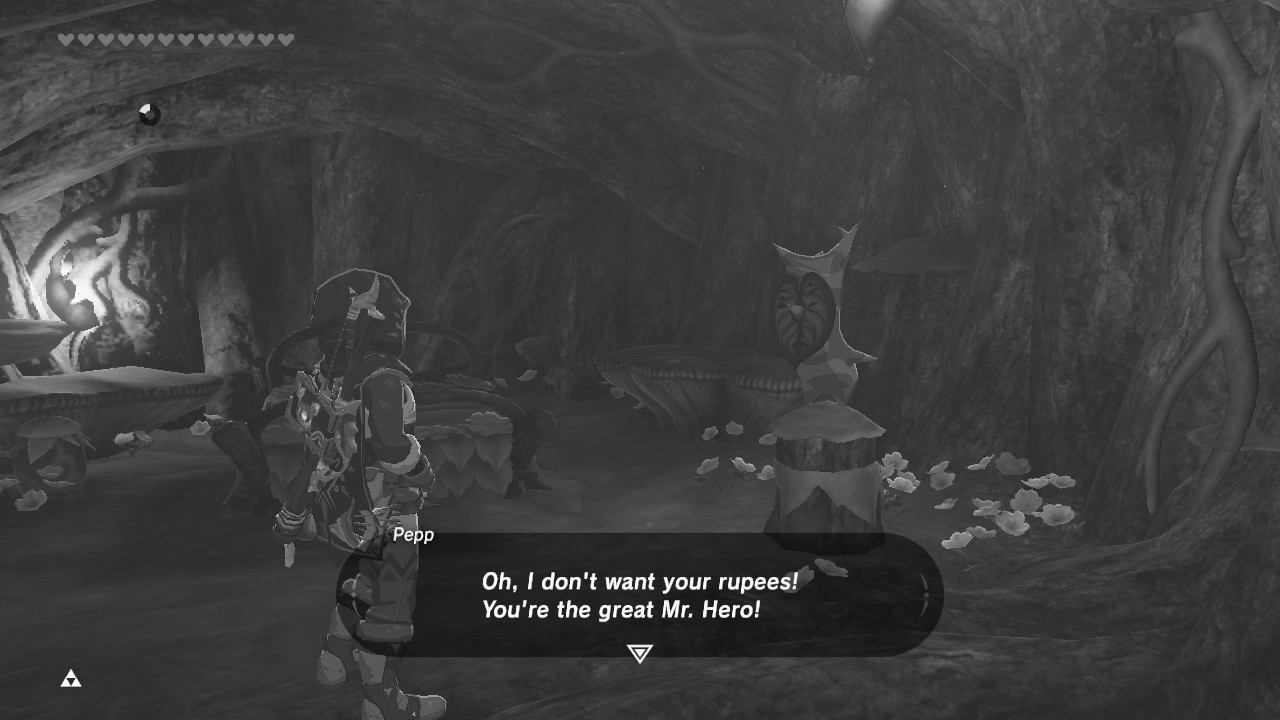
\includegraphics[width=\linewidth]{figure30.png}
        \caption{Kênh Y}
    \end{subfigure}
    \begin{subfigure}[H]{0.3\textwidth}
        \centering
        
\includegraphics[width=\linewidth]{figure31.png}
        \caption{Kênh Cb}
    \end{subfigure}
    \begin{subfigure}[H]{0.3\textwidth}
        \centering
        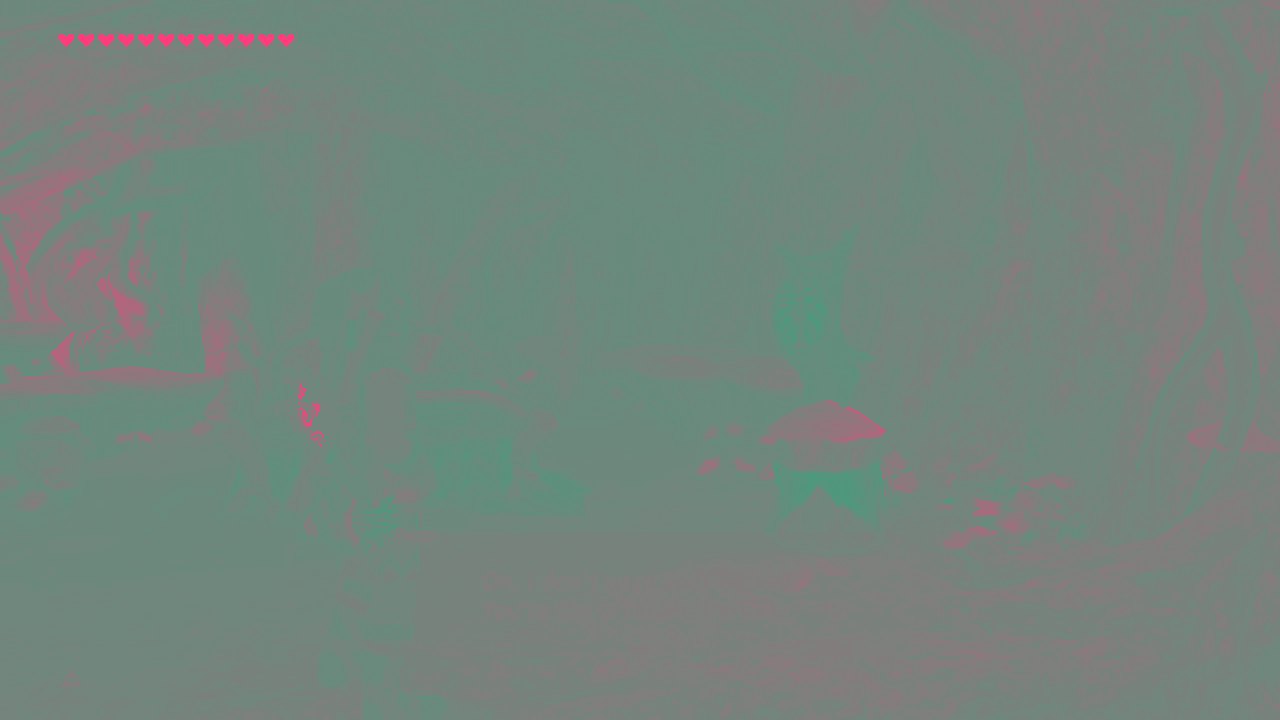
\includegraphics[width=\linewidth]{figure32.png}
        \caption{Kênh Cr}
    \end{subfigure}
    \caption{Biểu diễn giá trị các kênh màu của ảnh YCbCr.}
    \label{figure_ycbcr}
\end{figure}

Tuy nhiên, phương án này khiến ta không thể chỉnh sửa được độ sáng hay độ tương phản của ảnh, do các đặc điểm này được quyết định chủ yếu bởi kênh Y. Điều này khiến cho chất lượng ảnh đầu ra không tốt bằng chất lượng ảnh thực tế.

\subsection{PatchGAN}
\label{patchgan}

Thông thường, discriminator của GAN cho ra một kết quả phân loại thật/giả duy nhất cho toàn bộ ảnh. Thiết kế này hoạt động khá tốt trong phần lớn trường hợp, khi ta cần phải quan sát toàn bộ ảnh để có thể đưa ra kết quả đúng. Tuy nhiên, lượng dữ liệu đầu vào lớn có thể kiến model bỏ qua các chi tiết lỗi nhỏ như nhiễu hay nổ màu, khiến cho chất lượng ảnh đầu ra giảm.

Trong trường hợp của bài toán đổi màu ảnh nội soi, ta không cần phải sử dụng toàn bộ ảnh để phân loại thật - giả: chỉ cần dựa trên màu sắc và độ tương phản, ta có thể đoán được chế độ màu của ảnh. Lợi dụng đặc điểm này, ta có thể sử dụng discriminator PatchGAN để giảm bớt các chi tiết lỗi nhỏ.

\begin{figure}[H]
    \centering
    \begin{subfigure}[H]{0.48\textwidth}
        \centering
        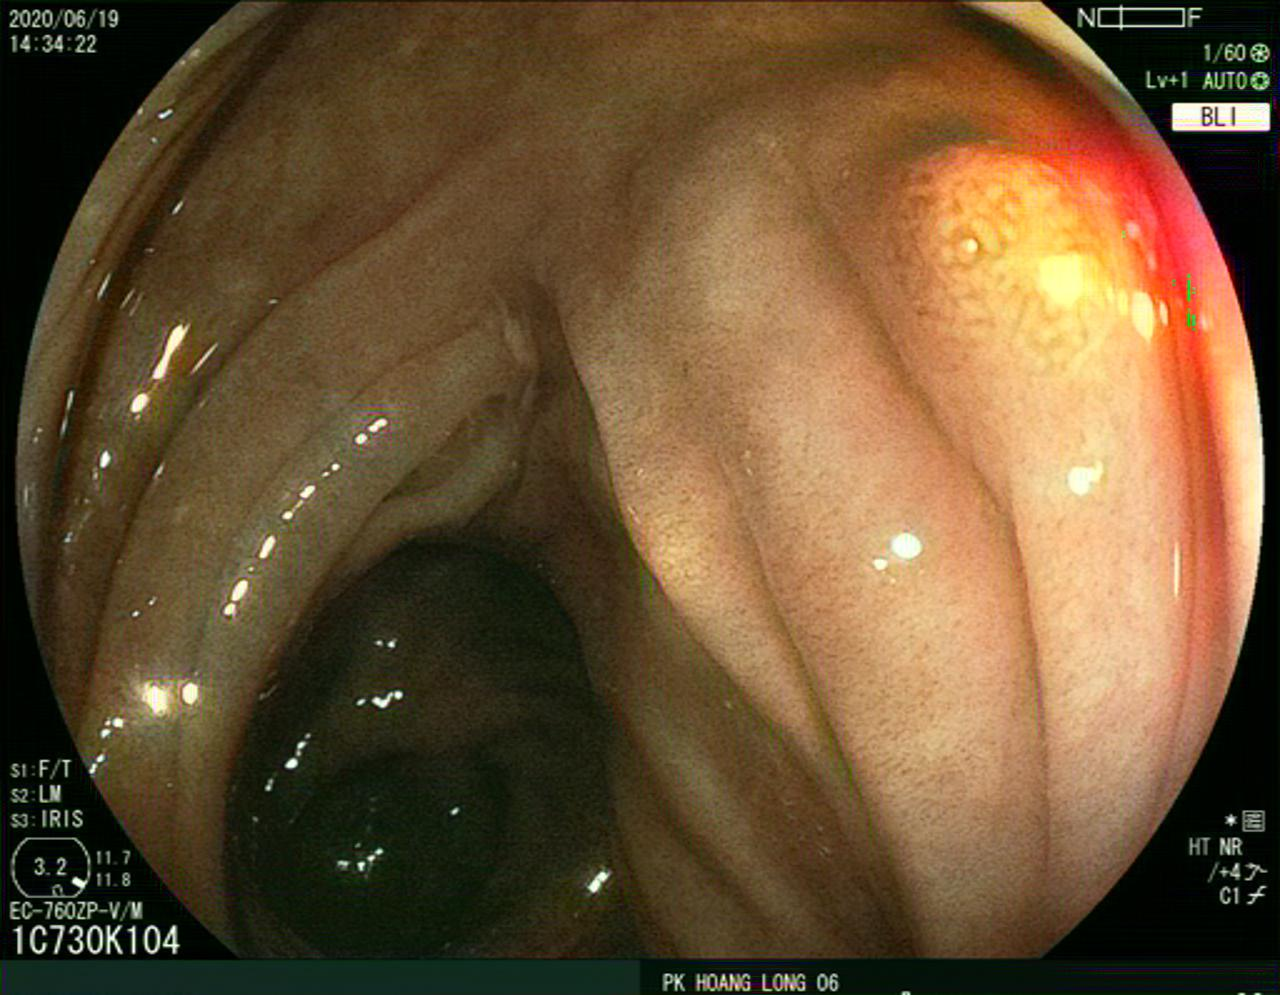
\includegraphics[width=\linewidth]{figure36.jpg}
        \caption{Sử dụng discriminator gốc}
    \end{subfigure}
    \begin{subfigure}[H]{0.48\textwidth}
        \centering
        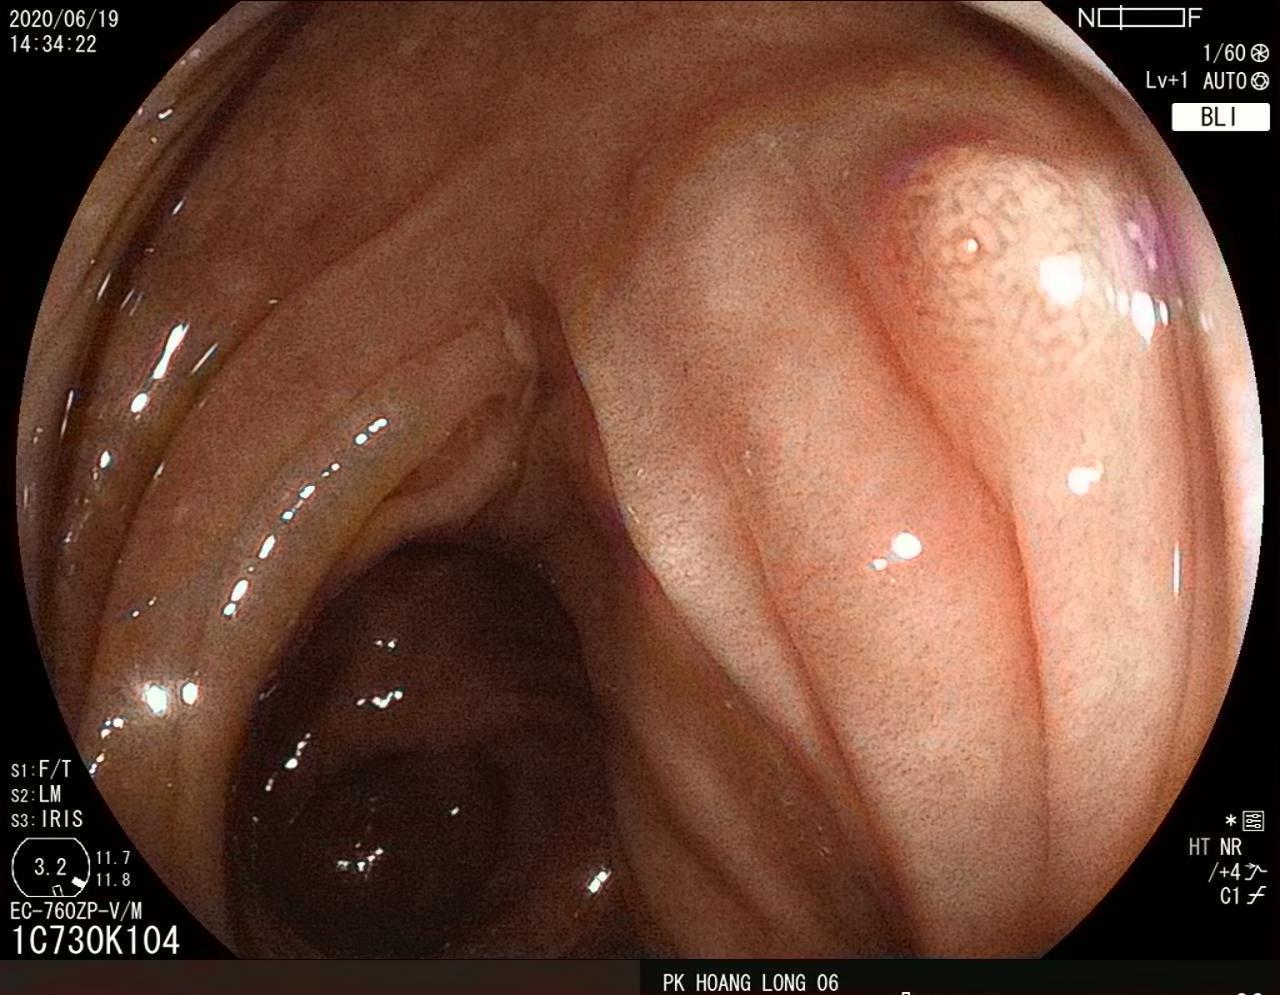
\includegraphics[width=\linewidth]{figure35.jpg}
        \caption{Sử dụng PatchGAN}
    \end{subfigure}
    \caption{So sánh kết quả chuyển đổi ảnh nội soi BLI sang WLI của mô hình StarGAN v2 sử dụng discriminator gốc và sử dụng discriminator PatchGAN. Discriminator gốc bỏ qua các điểm đốm xanh ở góc trên bên phải, trong khi PatchGAN bắt và loại bỏ được lỗi này.}
\end{figure}

PatchGAN là mô hình discriminator được để xuất trong nghiên cứu Pix2pix của các nhà khoa học thuộc trường Đại học California. PatchGAN sử dụng mạng convolutional để phân loại ảnh theo từng mảng (patch) nhỏ. Kết quả trung bình của tất cả các mảng sẽ được sử dụng làm kết quả phân loại cuối cùng.

\begin{figure}[H]
    \centering
    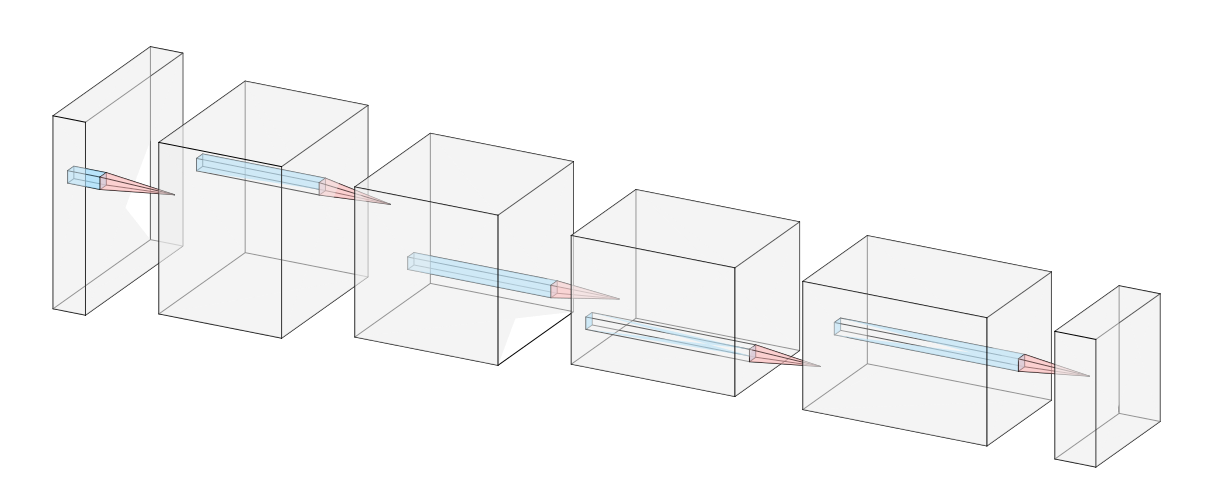
\includegraphics[width=\linewidth]{figure37.png}
    \caption{Minh họa mạng discriminator PatchGAN. Đầu ra của lớp convolutional cuối cùng có kích thước $ C_y \times W_y \times W_y $, trong đó $ C_y $ bằng với số lớp ảnh của bài toán. Mỗi một ô trên dữ liệu đầu ra này tương ứng với kết quả phân loại một vùng nhỏ trên ảnh gốc.}
\end{figure}

Vì làm việc vùng ảnh nhỏ, PatchGAN nhạy cảm với các tiểu tiết bị lỗi trên ảnh hơn các mạng discriminator bình thường, đặc biệt là khi kích thước ảnh lớn, lượng dữ liệu toàn cục nhiều.

\section{Thiết kế các thành phần mạng nơ-ron}

\subsection{Các khối mạng đặc biệt}

\subsubsection{Instance Normalization}

Ioffe và Szegedy đề xuất sử dụng lớp Batch Normalization \cite{DBLP:journals/corr/IoffeS15} để chuẩn hóa phân bố xác suất giá trị đầu vào của các lớp mạng học sâu. Công thức của lớp Batch Normalization có dạng:
$$ BN(x) = \gamma \times \cfrac{x - \mu(x)}{\phi(x)} + \beta $$
với $ \gamma $ và $ \beta $ là các tham số cần học, tương ứng với phương sai và giá trị kì vọng của phân bố xác suất mới. $ \mu(x) $ và $ \phi(x) $ là phương sai và giá trị kì vọng của lô dữ liệu đầu vào:
\begin{align*}
    \mu_c(x)  & = \cfrac{1}{NHW} \sum_{n = 1}^{N} \sum_{h = 1}^{H} \sum_{w = 1}^{W} x_{nchw}                       \\
    \phi_c(x) & = \sqrt{\cfrac{1}{NHW} \sum_{n = 1}^{N} \sum_{h = 1}^{H} \sum_{w = 1}^{W} (x_{nchw} - \mu_c(x))^2}
\end{align*}

Mục đích thiết kế ban đầu của lớp Batch Normalization là để tăng tốc độ học của mạng nơ-ron. Tuy nhiên, các nghiên cứu về sau chỉ ra lớp Batch Normalization cũng có thể được áp dụng vào việc chuyển đổi phong cách ảnh, bằng cách chuyển phân bố xác suất phong cách của ảnh gốc sang phong cách ảnh mục tiêu \cite{radford2015unsupervised}. Với cùng tư tưởng đó, Ulyanov và cộng sự cho ra đời lớp mạng Instance normalization \cite{DBLP:journals/corr/UlyanovVL16}, có nhiệm vụ thay đổi phân bố của từng cá thể dữ liệu thay vì thay đổi cả lô:
\begin{align*}
    \mu_{nc}(x)  & = \cfrac{1}{HW} \sum_{h = 1}^{H} \sum_{w = 1}^{W} x_{nchw}                     \\
    \phi_{nc}(x) & = \sqrt{\cfrac{1}{HW} \sum_{h = 1}^{H} \sum_{w = 1}^{W} (x_{nchw} - \mu(x))^2}
\end{align*}

Bằng cách học các bộ trọng số $ y $ và $ \beta $, lớp Instance Normalization có thể thực hiện biến đổi từ một phong cách (phân bố xác suất) này sang một phong cách (phân bố xác suất) khác.

\subsubsection{Adaptive Instance Normalization}

Adaptive Instance Normalization hay AdaIN là phiên bản cải tiến của Instance Normalization, cho phép biến đổi ảnh sang phong cách bất kì, quyết định bởi vector phong cách. Thay vì học trực tiếp một phân bố xác suất cố định, AdaIN học công thức biến đổi từ vector phong cách sang phân bố xác suất của nó:
\begin{align*}
    \gamma(s) & = W_{\gamma}s + b_{\gamma}                                \\
    \beta(s)  & = W_{\beta}s + b_{\beta}                                  \\
    BN(x)     & = \gamma(s) \times \cfrac{x - \mu(x)}{\phi(x)} + \beta(s)
\end{align*}

\subsubsection{Khối mạng Residual}

Như đã chỉ ra trong chương 2, quá trình luyện tập mô hình học máy có giám sát tương ứng với việc tìm ước lượng hàm $ \hat{f}(x) $ gần nhất so với quan hệ thực tế $ f(x) $. Gọi $ \hat{F}_n(x) $ là tập hợp tất cả các hàm $ \hat{f}(x) $ mà mô hình $ n $ lớp mạng có thể biểu diễn. Khi số lượng lớp mạng gia tăng, độ phức tạp của ước lượng hàm cũng tăng lên tương ứng. Nếu:
\begin{equation}
    \hat{F}_{n-1}(x) \subseteq \hat{F}_n(x)
    \label{eq:res}
\end{equation}
ta hiểu là không gian hàm mở rộng cùng với số lớp mạng, gia tăng khả năng $ \hat{f}(x) $ tiếp cận với $ f(x) $.

Tuy nhiên, trên thực tế điều này có thể không xảy ra - miền $ \hat{F}_n(x) $ có thể không chứa $ \hat{F}_{n-1}(x) $, và các hàm thuộc $ \hat{F}_n(x) $ có thể không tiến tới $ f(x) $ như kì vọng. Nếu mạng nơ-ron có thể học được hàm đồng nhất $ f(x) = x $ một cách đơn giản, ta đảm bảo điều kiện \ref{eq:res}, dẫn tới việc không gian hàm luôn mở rộng khi số lượng lớp mạng gia tăng. Đây chính là tư tưởng đằng sau mô hình mạng Residual, được đề xuất bởi He và cộng sự vào năm 2015 \cite{he2015deep}.

\begin{figure}[H]
    \centering
    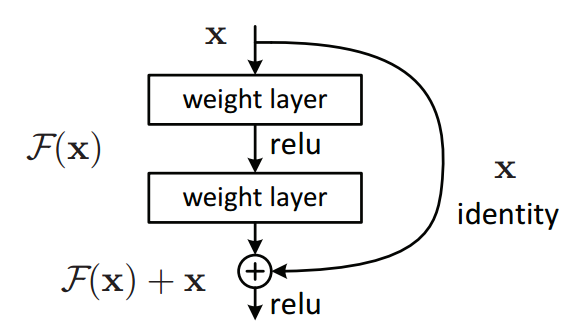
\includegraphics[width=0.7\linewidth]{figure33.png}
    \caption{Thiết kế của một khối Residual cơ bản.}
\end{figure}

Mạng Residual cơ bản sử dụng các khối Residual, mỗi khối bao gồm một phép biến đổi tuyến tính $ z_1 = W_1x $, một trọng số tổng hợp $ W_2 $ và hai hàm kích hoạt ReLU $ f_1(x) $, $ f_2(x) $. Khối Residual tổng hợp giá trị đầu vào $ x $ với kết quả đã kích hoạt của phép biến đổi tuyến tính để cho ra kết quả cuối cùng:
\begin{align*}
    z_1 & = W_1x       \\
    a_1 & = f_1(z_1)   \\
    z_2 & = W_1z_1 + x \\
    y   & = f_2(z_2)
\end{align*}

Trong trường hợp cần phải học hàm đồng nhất, khối Residual chỉ cần tối ưu trọng số $ W_2 $ về 0. Khi đó, nếu tất cả các thành phần của $ x $ đều dương, ta có $ y = f_2(f_1(x)) = x $.

Tổng quát hơn, ta có thể bổ sung thêm một ma trận trọng số $ W_3 $ để tổng hợp các thành phần của $ x $ với các trọng số khác nhau.
$$ y = f_2(z_2 + W_3x) $$

Trường hợp kích thước của $ x $ và $ y $ khác nhau, ta cần sử dụng $ W_3 $ để nén $ x $ về kích cỡ của $ y $.

Trong mô hình StarGAN v2, khối Residual được sử dụng trong generator, discriminator và style encoder để nén và giải nén dữ liệu ảnh. Điểm khác biệt duy nhất giữa khối mạng nén và giải nén nằm ở lớp pooling và normalization - khối nén sử dụng Average Pooling để giảm một nửa kích cỡ dữ liệu và Instance Normalization để chuẩn hóa, trong khi khối giải nén sử dụng Nearest Interpolation để gấp đôi kích cỡ dữ liệu và AdaIN để chuyển đổi phong cách.

Kiến trúc cụ thể của một khối Residual được mô tả dưới đây:

\begin{table}[H]
    \centering
    \begin{subtable}[H]{.48\textwidth}
        \begin{adjustbox}{width=\textwidth}
            \begin{tabular}{c c c}
                Lớp mạng        & Hàm kích hoạt & Đầu ra                                          \\
                \hline
                Input           &               & $ C \times W \times W $                         \\
                \hline
                \textbf{\textit{Nhánh chính}}                                                     \\
                Instance Norm   & Leaky ReLU    & $ C \times W \times W $                         \\
                Conv3x3         &               & $ C \times W  \times W $                        \\
                Average Pooling &               & $ C \times \cfrac{W}{2}  \times \cfrac{W}{2} $  \\
                Instance Norm   & Leaky ReLU    & $ C \times \cfrac{W}{2}  \times \cfrac{W}{2} $  \\
                Conv3x3         &               & $ C' \times \cfrac{W}{2}  \times \cfrac{W}{2} $ \\
                \hline
                \textbf{\textit{Nhánh phụ}}                                                       \\
                Conv1x1         &               & $ C' \times W  \times W $                       \\
                Average Pooling &               & $ C' \times \cfrac{W}{2}  \times \cfrac{W}{2} $ \\
                \hline
                \textbf{\textit{Tổng hợp}}                                                        \\
                Add             &               & $ C' \times \cfrac{W}{2}  \times \cfrac{W}{2} $ \\
            \end{tabular}
        \end{adjustbox}
    \end{subtable}
    \begin{subtable}[H]{.48\textwidth}
        \begin{adjustbox}{width=\textwidth}
            \begin{tabular}{c c c}
                Lớp mạng    & Hàm kích hoạt & Đầu ra                      \\
                \hline
                Input       &               & $ C \times W \times W $     \\
                \hline
                \textbf{\textit{Nhánh chính}}                             \\
                AdaIN       & Leaky ReLU    & $ C \times W \times W $     \\
                Interpolate &               & $ C \times 2W  \times 2W $  \\
                Conv3x3     &               & $ C' \times 2W  \times 2W $ \\
                AdaIN       & Leaky ReLU    & $ C' \times 2W \times 2W $  \\
                Conv3x3     &               & $ C' \times 2W  \times 2W $ \\
                \hline
                \textbf{\textit{Nhánh phụ}}                               \\
                Interpolate &               & $ C \times 2W  \times 2W $  \\
                Conv1x1     &               & $ C' \times 2W  \times 2W $ \\
                \hline
                \textbf{\textit{Tổng hợp}}                                \\
                Add         &               & $ C' \times 2W  \times 2W $ \\
            \end{tabular}
        \end{adjustbox}
    \end{subtable}
    \caption{Kiến trúc một khối Residual trong mô hình StarGAN v2.}
\end{table}

\subsection{Kiến trúc các mạng thành phần}

\subsubsection{Generator}

Generator được xây dựng theo phong cách của mạng autoencoder: Đầu tiên, ảnh gốc ở không gian màu YCbCr kích cỡ $ 1024 \times 1024 $ được đưa vào một loạt các khối Residual để nén xuống thành dữ liệu nén có kích thước $ 16 \times 16 $. Sau đó, dữ liệu nén này lại được đi qua các khối Residual để giải nén và kết hợp cùng với vector phong cách để cho ra ảnh mới, có kích thước bằng với ảnh ban đầu. Như đã nói ở mục \ref{ycbcr-colorspace}, generator chỉ sinh mới hai kênh Cb và Cr để ghép với kênh Y của ảnh gốc.

\begin{table}[H]
    \centering
    \begin{tabular}{c c c}
        Lớp mạng          & Hàm kích hoạt & Đầu ra                         \\
        \hline
        Input             &               & $ 3 \times 1024 \times 1024 $  \\
        Conv1x1           &               & $ 32 \times 1024 \times 1024 $ \\
        Residual nén      &               & $ 64 \times 512 \times 512 $   \\
        Residual nén      &               & $ 128 \times 256 \times 256 $  \\
        Residual nén      &               & $ 256 \times 128 \times 128 $  \\
        Residual nén      &               & $ 512 \times 64 \times 64 $    \\
        Residual nén      &               & $ 512 \times 32 \times 32 $    \\
        Residual nén      &               & $ 512 \times 16 \times 16 $    \\
        Residual nén      &               & $ 512 \times 16 \times 16 $    \\
        Residual nén      &               & $ 512 \times 16 \times 16 $    \\
        Residual giải nén &               & $ 512 \times 16 \times 16 $    \\
        Residual giải nén &               & $ 512 \times 16 \times 16 $    \\
        Residual giải nén &               & $ 512 \times 32 \times 32 $    \\
        Residual giải nén &               & $ 512 \times 64 \times 64 $    \\
        Residual giải nén &               & $ 256 \times 128 \times 128 $  \\
        Residual giải nén &               & $ 128 \times 256 \times 256 $  \\
        Residual giải nén &               & $ 64 \times 512 \times 512 $   \\
        Residual giải nén &               & $ 32 \times 1024 \times 1024 $ \\
        Instance Norm     & Leaky ReLU    & $ 32 \times 1024 \times 1024 $ \\
        Conv1x1           &               & $ 2 \times 1024 \times 1024 $  \\
    \end{tabular}
    \caption{Kiến trúc của mạng generator}
\end{table}

\subsubsection{Style Encoder}

Style Encoder nhận vào ảnh thật cùng với chỉ số lớp của ảnh, và cho ra một vector phong cách có 128 chiều. Kiến trúc của mạng bao gồm phần mạng nén chung giữa tất cả các lớp ảnh mục tiêu, và phần mạng riêng sinh kết quả cho mỗi lớp. Khi tối ưu Style Encoder, chỉ có phần mạng chung và phần mạng riêng tương ứng với lớp của ảnh đầu vào được tối ưu.

\begin{table}[H]
    \centering
    \begin{tabular}{c c c}
        Lớp mạng        & Hàm kích hoạt & Đầu ra                         \\
        \hline
        Input           &               & $ 3 \times 1024 \times 1024 $  \\
        \hline
        \textbf{\textit{Phần chung}}                                     \\
        Conv1x1         &               & $ 32 \times 1024 \times 1024 $ \\
        Residual nén    &               & $ 64 \times 512 \times 512 $   \\
        Residual nén    &               & $ 128 \times 256 \times 256 $  \\
        Residual nén    &               & $ 256 \times 128 \times 128 $  \\
        Residual nén    &               & $ 512 \times 64 \times 64 $    \\
        Residual nén    &               & $ 512 \times 32 \times 32 $    \\
        Residual nén    &               & $ 512 \times 16 \times 16 $    \\
        Residual nén    &               & $ 512 \times 8 \times 8 $      \\
        Residual nén    & Leaky ReLU    & $ 512 \times 4 \times 4 $      \\
        Conv4x4         & Leaky ReLU    & $ 512 \times 1 \times 1 $      \\
        \hline
        \textbf{\textit{Phần riêng}}                                     \\
        Fully Connected &               & 128
    \end{tabular}
    \caption{Kiến trúc của mạng Style Encoder}
\end{table}

\subsubsection{Mapping Network}

Mapping Network nhận vào vector latent có 16 chiều, cùng với chỉ số của một lớp, và cho ra một vector phong cách có 128 chiều, tương ứng với vector latent và đảm bảo ảnh được biểu diễn thuộc về lớp đã chỉ định. Giống như Style Encoder, Mapping Network cũng có hai phần chung và riêng, và chỉ có phần riêng tương ứng với lớp được chỉ định được tối ưu trong quá trình học.

\begin{table}[H]
    \centering
    \begin{tabular}{c c c}
        Lớp mạng        & Hàm kích hoạt & Đầu ra  \\
        \hline
        Input           &               & $ 16 $  \\
        \hline
        \textbf{\textit{Phần chung}}              \\
        Fully Connected & ReLu          & $ 512 $ \\
        Fully Connected & ReLu          & $ 512 $ \\
        Fully Connected & ReLu          & $ 512 $ \\
        Fully Connected & ReLu          & $ 512 $ \\
        \hline
        \textbf{\textit{Phần riêng}}              \\
        Fully Connected & ReLu          & $ 512 $ \\
        Fully Connected & ReLu          & $ 512 $ \\
        Fully Connected & ReLu          & $ 512 $ \\
        Fully Connected &               & $ 128 $
    \end{tabular}
    \caption{Kiến trúc của mạng Mapping Network}
\end{table}

\subsubsection{Discriminator}

Discriminator nhận vào ảnh thật cùng với chỉ số lớp của ảnh, và cho ra giá trị trong khoảng $ [0, 1] $ đánh giá ảnh có phải là ảnh thật của lớp được chỉ định hay không. Như đã giới thiệu trong mục \ref{patchgan}, discriminator này sử dụng mạng CNN để phân loại thật giả từng mảng $ 70 \times 70 $ trên ảnh gốc, sau đó lấy kết quả trung bình để cho ra kết quả phân loại cuối cùng.

\begin{table}[H]
    \centering
    \begin{tabular}{c c c}
        Lớp mạng   & Hàm kích hoạt & Đầu ra                        \\
        \hline
        Input      &               & $ 3 \times 1024 \times 1024 $ \\
        \hline
        Conv4x4    & Leaky ReLU    & $ 64 \times 512 \times 512 $  \\
        Conv4x4    &               & $ 128 \times 256 \times 256 $ \\
        Batch Norm & Leaky ReLU    & $ 128 \times 256 \times 256 $ \\
        Conv4x4    &               & $ 256 \times 128 \times 128 $ \\
        Batch Norm & Leaky ReLU    & $ 256 \times 128 \times 128 $ \\
        Conv4x4    &               & $ 512 \times 127 \times 127 $ \\
        Batch Norm & Leaky ReLU    & $ 512 \times 127 \times 127 $ \\
        Conv4x4    & Leaky ReLU    & $ 4 \times 126 \times 126 $   \\
        Average    & Sigmoid       & 4
    \end{tabular}
    \caption{Kiến trúc của mạng discriminator}
\end{table}

\section{Hàm mục tiêu}

Tất cả các hàm mục tiêu dưới đây đều được tính toán hai lần với vector phong cách $ s $ sinh ra bởi Style Encoder (nhằm tối ưu cho bài toán sinh ảnh dựa theo ảnh đối chiếu) và $ s $ sinh ra bởi Mapping Network (nhằm tối ưu cho bài toán sinh ảnh theo phong cách ngẫu nhiên).

\subsection{Hàm Minimax}

Tương tự như các mô hình GAN truyền thống, ta sử dụng hàm Minimax để tối ưu các mạng thành phần:
$$ L_{adv} =  E_{x,y} [\log(D_y(x))] + E_{x,y,y'} [\log(1 - D_{y'}(G(x,s)))] $$
với $ x $, $ y $ là ảnh đầu vào và lớp của ảnh, $ y' $ là lớp mục tiêu, $ s $ là một vector phong cách của ảnh thuộc lớp $ y' $. Discriminator cố gắng tối đa hóa hàm mục tiêu này này (nhận diện ảnh thật/giả tốt hơn) trong khi generator cố gắng tối thiểu nó (đánh lừa discriminator tốt hơn).

\subsection{Hàm tái tạo phong cách (style reconstruction loss)}

Để hướng generator sử dụng vector phong cách $ s $ khi sinh ảnh, ta sử dụng hàm thiệt hại tái tạo phong cách, biểu diễn sai số giữa phong cách được truyền vào generator và phong cách của ảnh được sinh ra:
$$ L_{sty} = E_{x,y',s} [|s - E_{y'}(G(x, s))|] $$
trong đó $ E_{y}(x) $ là kết quả của Style Encoder khi sinh vector phong cách của ảnh $ x $ theo lớp $ y $. Generator hướng tới tối thiểu giá trị $ L_{sty} $ bằng cách sử dụng tri thức đã được mã hóa trong $ s $ để tạo ra ảnh mới có phong cách mà Style Encoder có thể giải mã được.

\subsection{Hàm đa dạng phong cách (style diversification loss)}

Mục tiêu xây dựng mô hình StarGAN v2 là để sinh ra ảnh với nhiều phong cách đa dạng khác nhau. Ta mô hình hóa mục tiêu này bằng độ đo đa dạng phong cách:
$$ E_{x,y',s_1,s_2} \left[\left|\cfrac{G(x,s_1) - G(x,s_2)}{s_1 - s_2}\right|\right] $$

Với hai vector phong cách $ s_1 $ và $ s_2 $ bất kì, ta kì vọng ảnh đầu ra sử dụng hai vector này càng khác nhau khi $ s_1 $ và $ s_2 $ càng xa nhau. Tuy nhiên, khi luyện tập mô hình thực tế, mẫu số $ | s_1 - s_2 | $ thường rất nhỏ, khiến cho giá trị của độ đo này trở nên rất lớn, làm quá trình luyện tập trở nên không ổn định. Thay vào đó, ta chỉ sử dụng phần tử số hàm hàm mục tiêu:
$$ L_{ds} = E_{x,y',s_1,s_2} \left[\left|G(x,s_1) - G(x,s_2)\right|\right] $$

\subsection{Hàm cycle consistency}

Hàm mục tiêu cycle consistency của StarGAN v2 giống như hàm cycle consistency được sử dụng bởi StarGAN phiên bản đầu tiên:
$$ L_{cyc} = E_{x \in X} [|G_B(G_A(x)) - x|] + E_{y \in Y} [|G_A(G_B(y)) - y|] $$

\subsection{Hàm regularization R1}

Hàm regularization R1 không liên quan tới các mục tiêu của StarGAN v2. Thay vào đó, R1 giúp sự hội tụ của StarGAN v2 ổn định hơn.

Nhắc lại từ mục \ref{gan}, quá trình tối ưu mô hình GAN là một trò chơi Minimax giữa generator và discriminator. Trạng thái tối ưu của mô hình GAN vì thế cũng chính là điểm cân bằng Nash giữa hai mạng này - khi khả năng sinh ảnh giả của generator ngang bằng với khả năng phân biệt ảnh thật/giả của discriminator. Khi cân bằng Nash xảy ra, generator sinh được ảnh đánh lừa được discriminator, discriminator sẽ phải dự đoán ngẫu nhiên. Sai số từ những lần dự đoán ngẫu nhiên này sẽ khiến cho discriminator bị cập nhật sai hướng và giảm chất lượng, kéo chất lượng của generator giảm tương ứng.

Mescheder, Geiger và Nowozin \cite{DBLP:journals/corr/abs-1801-04406} chỉ ra rằng để mô hình GAN hội tụ ổn định hơn, ta cần ngăn cản discriminator rời khỏi điểm cân bằng Nash. Một phương pháp đơn giản để thực hiện điều này là sử dụng hàm regularization R1:
$$ R_1 = \cfrac{1}{2} E_{x \in X_{real}}[|\nabla D(x)|^2] $$

Gradient cập nhật của discriminator càng lớn, giá trị của $ R_1 $ càng lớn. Tối ưu $ R_1 $ đồng nghĩa với việc kiểm soát tốc độ cập nhật của discriminator, khiến cho discriminator khó rời khỏi trạng thái ổn định hơn.  Vì ta không thể biết được khi nào xảy ra cân bằng Nash (generator đánh lừa được discriminator), ta chỉ áp dụng hàm R1 với đầu vào discriminator là các ảnh thật, không áp dụng với dữ liệu đầu ra của generator.

\subsection{Hàm mục tiêu tổng quát}

Hàm mục tiêu tổng quát được tính bằng cách tính tổng hệ số của các hàm mục tiêu kể trên:
$$ L = L_{adv} + \lambda_{sty} L_{sty} - \lambda_{ds} L_{ds} + \lambda_{cyc} L_{cyc} + \lambda_{reg} R_1  $$
trong đó $ \lambda_{sty} $, $ \lambda_{ds} $, $ \lambda_{cyc} $ và $ \lambda_{reg} $ là các hệ số được chọn bởi người dùng. Nghiên cứu gốc khuyến khích giảm dần $ \lambda_{ds} $ qua thời gian để quá trình luyện tập ổn định hơn.

Trên thực tế, discriminator chỉ bị ảnh hưởng tới $ L_{adv} $ và R1, trong khi generator, Style Encoder và Mapping Network bị ảnh hưởng bởi tất cả các hàm mục tiêu trừ hàm R1. Do đó ta chỉ cần tính các giá trị hàm tương ứng khi tối ưu các mạng thành phần.

\chapter{Luyện tập mô hình và đánh giá}

Chương này sẽ trình bày về quá trình thu thập, tiền xử lý dữ liệu ảnh nội soi và luyện tập mô hình StarGAN v2 để giải bài toán chuyển đồi màu ảnh nội soi.

\section{Thu thập và tiền xử lý dữ liệu}

Bộ dữ liệu ảnh nội soi được thu thập bởi các bác sĩ của Viện nghiên cứu và đào tạo tiêu hóa gan mật IGH, thông qua hệ thống quản lý dữ liệu ảnh nội soi Polyp-Labeler. Đây là sản phẩm do em thiết kế cho bộ môn Project 3, thuộc chương trình học của trường. Chương \ref{application-polyp-labeler} sẽ giới thiệu ứng dụng của mô hình StarGAN v2 vào hệ thống này để cài đặt chức năng đổi màu ảnh nội soi.

\begin{figure}[H]
    \centering
    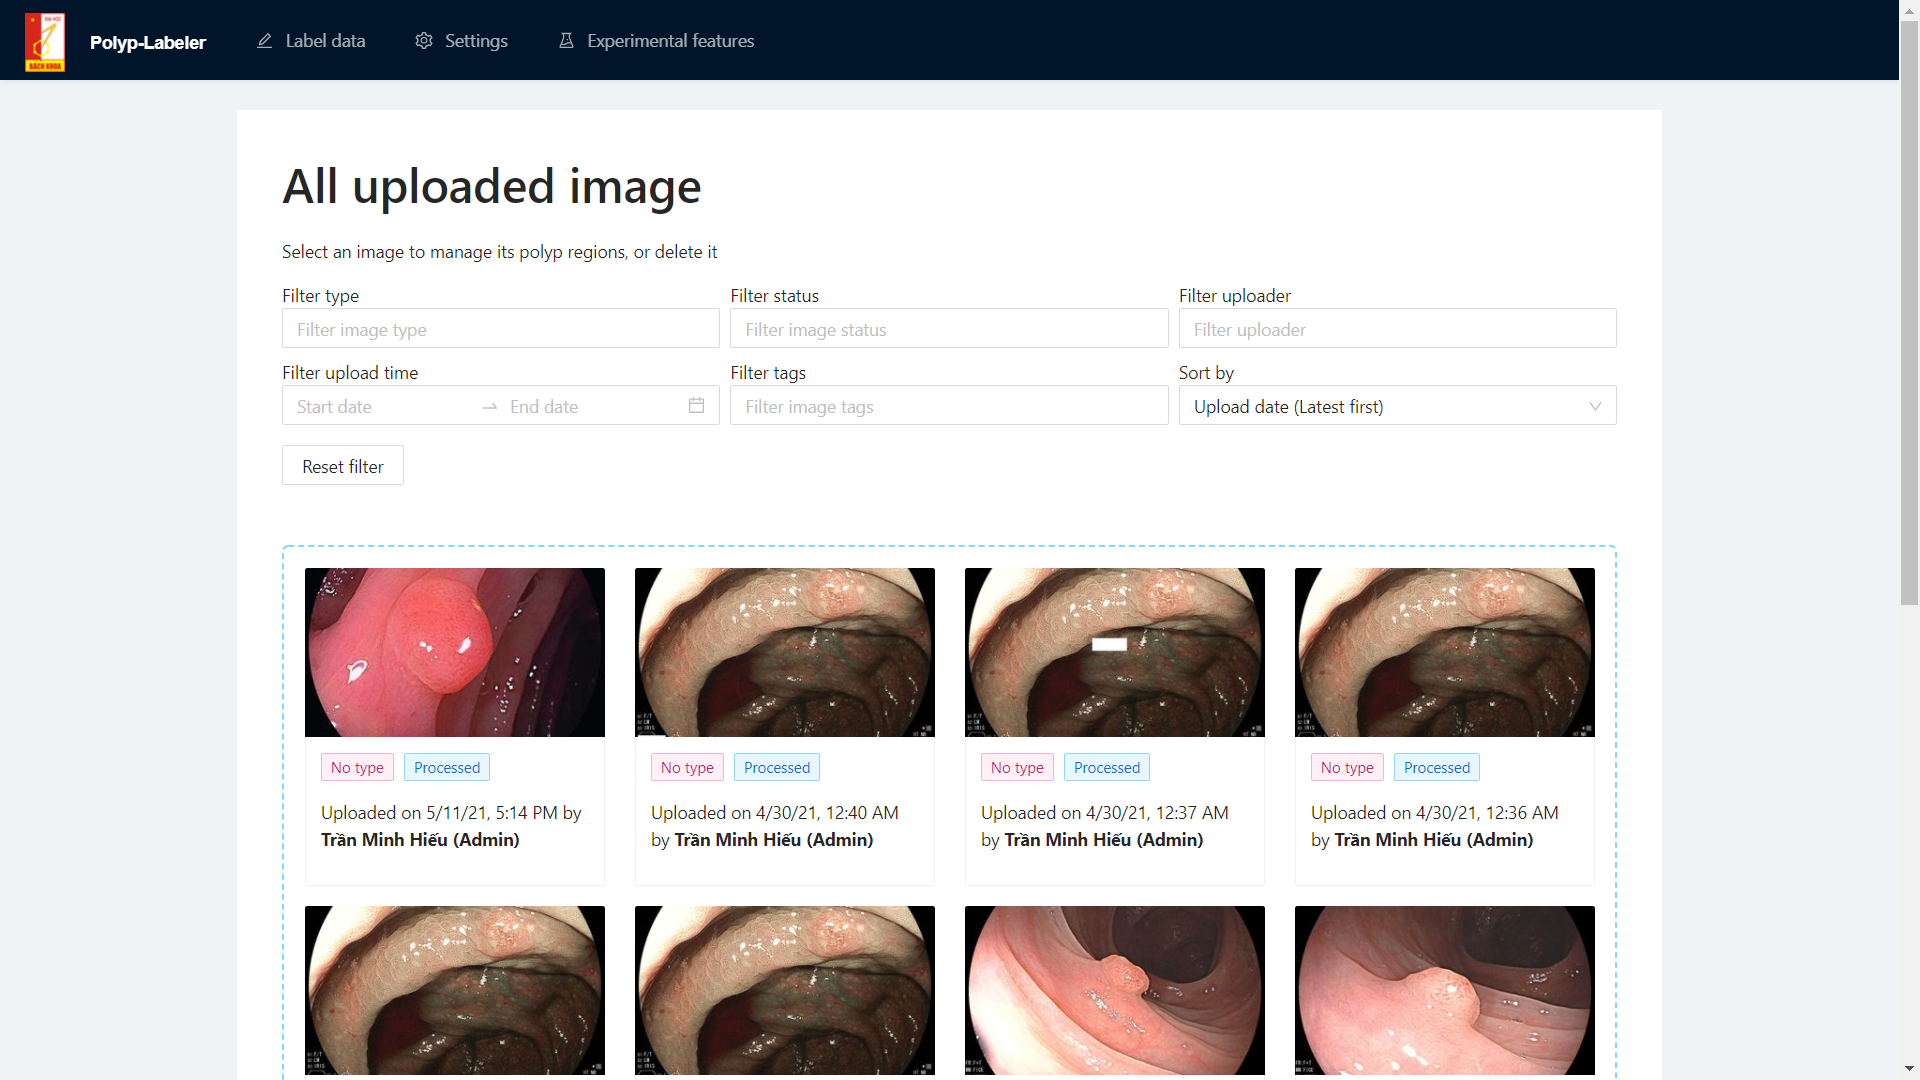
\includegraphics[width=0.7\linewidth]{figure34.png}
    \caption{Hệ thống quản lý dữ liệu ảnh nội soi Polyp-Labeler.}
\end{figure}

Bộ dữ liệu bao gồm 8000 ảnh nội soi đại tràng với nhiều kích cỡ khác nhau, bao gồm ảnh thuộc 4 chế độ màu BLI, FICE, LCI và WLI, mỗi chế độ có 2000 ảnh. Trước khi đưa vào mô hình để luyện tập, các file ảnh sẽ được tiền xử lý theo trình tự sau:
\begin{enumerate}
    \item Xoay ngẫu nhiên theo cả hai chiều kim đồng hồ, tối đa 10 độ.
    \item Di dịch ảnh ngẫu nghiên theo cả hai chiều, tối đa 1\% kích thước ảnh.
    \item Phóng to hoặc thu nhỏ ngẫu nhiên nội dung ảnh, tối đa 20\%.
    \item Ngẫu nhiên lật ảnh theo chiều dọc hoặc chiều ngang.
    \item Thay đổi kích thước ảnh thành $ 512 \times 512 $.
    \item Biến đổi ảnh thành không gian màu YCbCr.
    \item Chuẩn hóa các giá trị màu trong ảnh về miền $ [0, 1] $.
\end{enumerate}

Các bước từ 1 đến 4 cho phép ta gia tăng số lượng ảnh từ bộ dữ liệu ảnh ít ỏi, đồng thời cũng giúp cải thiện chất lượng của mô hình: Do ảnh nội soi được lấy từ nhiều thiết bị khác nhau, mỗi thiết bị có một giao diện đồ họa khác nhau, mô hình có thể bị overfitting vào phần giao diện đồ họa của ảnh và cho ra kết quả kém chất lượng.

\begin{figure}[H]
    \centering
    \begin{subfigure}[H]{0.48\textwidth}
        \centering
        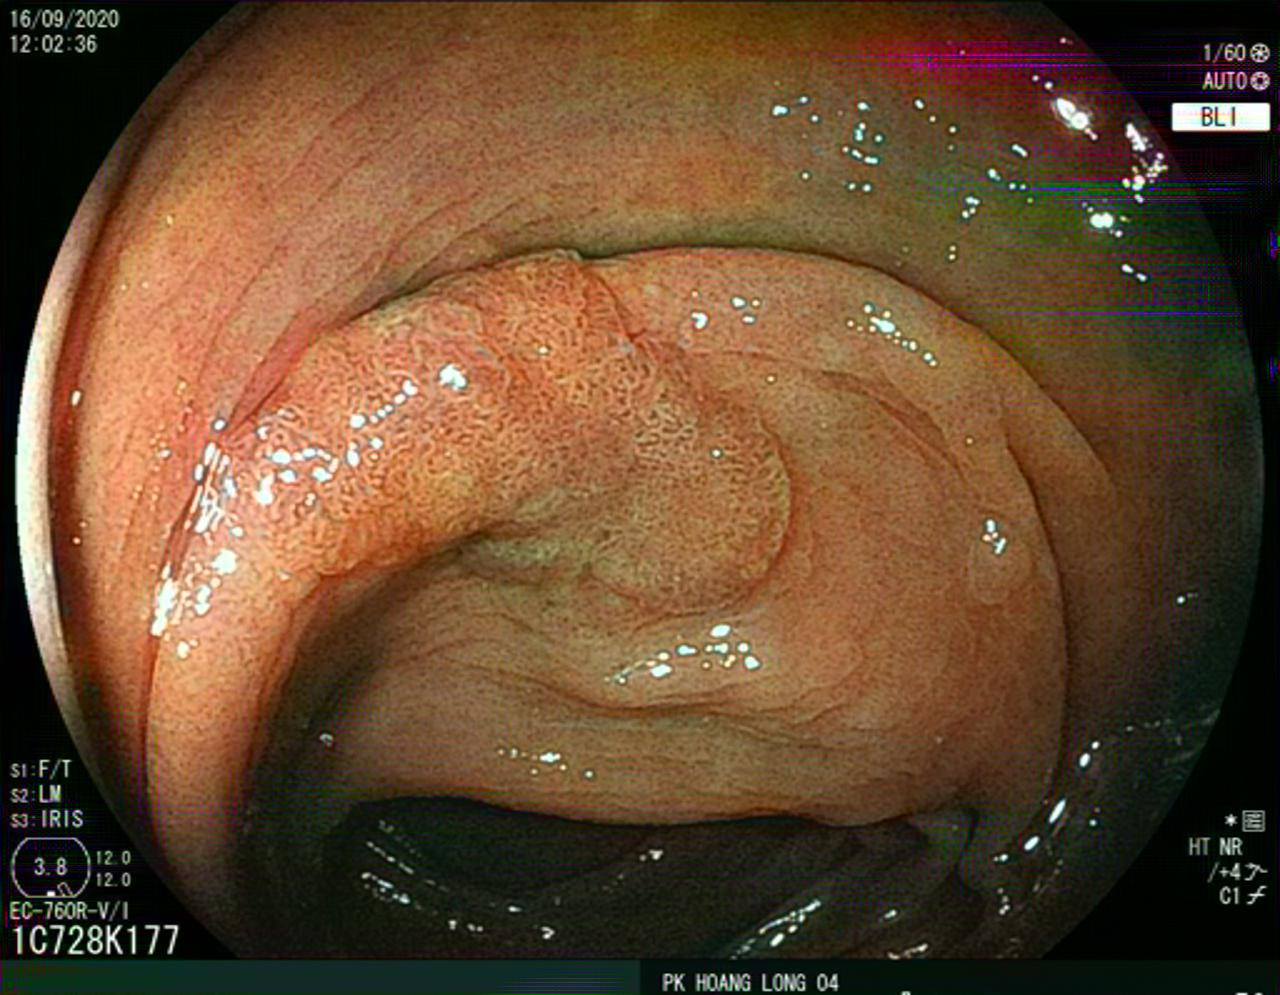
\includegraphics[width=\linewidth]{figure38.jpeg}
    \end{subfigure}
    \begin{subfigure}[H]{0.48\textwidth}
        \centering
        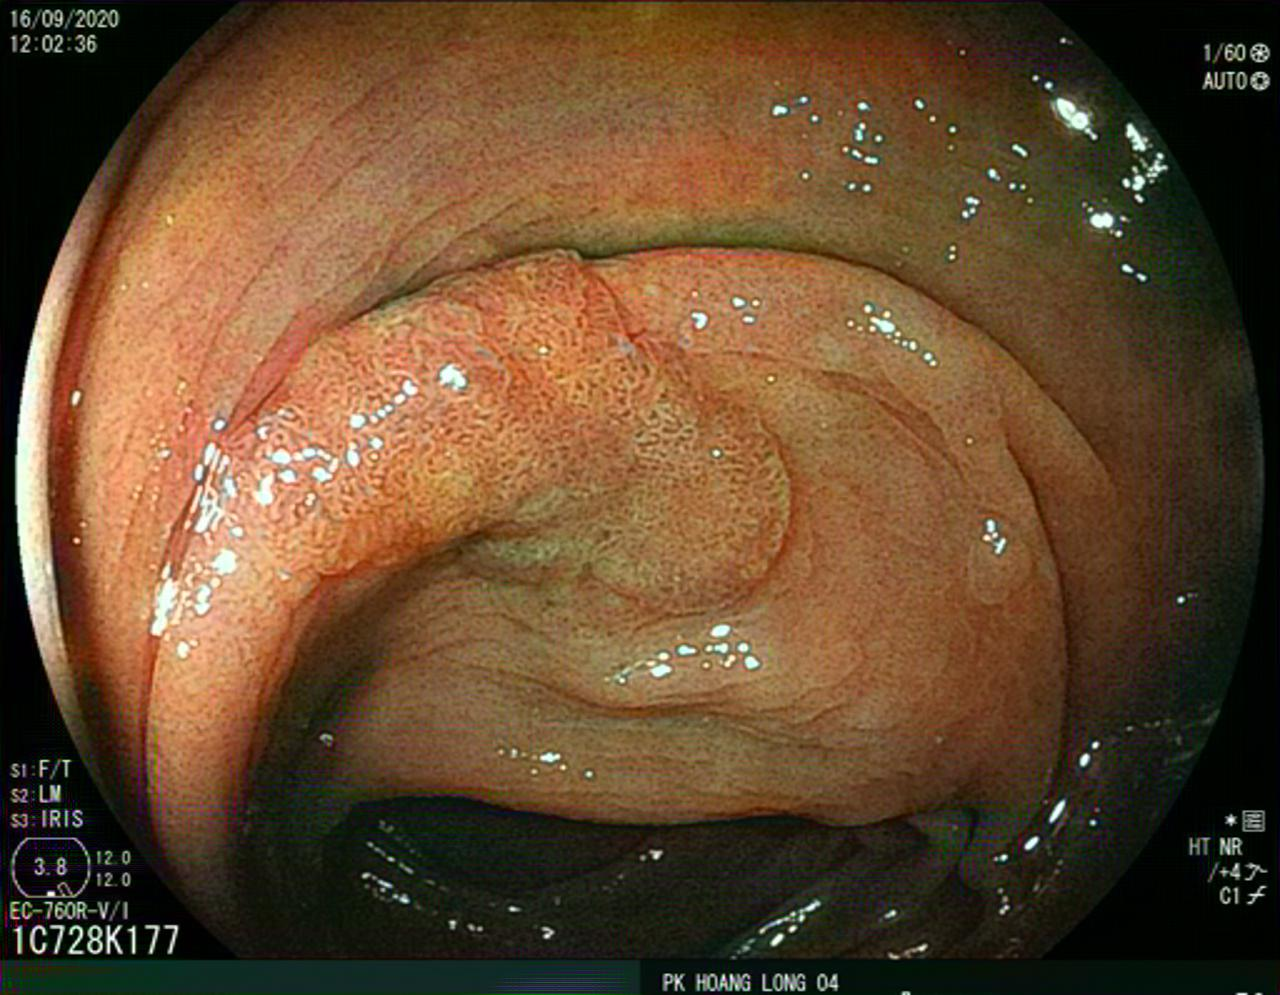
\includegraphics[width=\linewidth]{figure39.jpeg}
    \end{subfigure}
    \caption{Hai ảnh chuyển đổi từ chế độ BLI sang WLI bằng mô hình StarGAN v2 không xoay ảnh khi tiền xử lý dữ liệu. Ảnh bên phải là ảnh bên trái sau khi loại bỏ ô vuông trắng ở góc trên bên phải. Tất cả các ảnh thuộc chế độ màu WLI đều không có chi tiết này, trong khi tất cả các ảnh thuộc chế độ BLI đều có. Loại bỏ ô vuông trắng cũng loại bỏ hiện tượng lỗi ở ảnh trái, chứng tỏ lỗi bị gây ra do mô hình không biết xử lý ô vuông trắng khi chuyển sang chế độ WLI như thế nào.}
\end{figure}

Bước 5 cho phép ảnh lọt vừa kích thước đầu vào của mô hình. Bước 6 được giải thích ở mục \ref{ycbcr-colorspace}. Bước 7 giúp ổn định quá trình luyện tập - các số thực trong khoảng $ [0, 1] $ được biểu diễn chính xác nhất trên máy tính, và phép tính trong khoảng này ít có khả năng bùng nổ thành giá trị lớn, gây tràn miền giá trị biểu diễn.

\section{Môi trường luyện tập}

Chương trình huấn luyện mô hình StarGAN v2 được cài đặt bằng ngôn ngữ Python 3.8.6, sử dụng thư viện PyTorch. Chương trình sử dụng thuật toán tối ưu Adam theo lô, mỗi lô có 4 ảnh, chạy qua 50 nghìn bước lặp trên một GPU Nvidia GeForce RTX 3090 trong khoảng thời gian 2 ngày. Các tham số mô hình được lưu lại sau mỗi 2000 bước lặp để đánh giá chất lượng và sử dụng về sau.

Các hệ số được sử dụng cho quá trình luyện tập bao gồm:
\begin{itemize}
    \item $ \lambda_{sty} = \lambda_{ds} = \lambda_{cyc} = \lambda_{reg} = 1 $. $ \lambda_{ds} $ giảm về 0 một cách tuyến tính sau 100 nghìn bước lặp.
    \item Learning rate cho generator, Style Encoder và discriminator bằng $ 10^{-4} $.
    \item Learning rate cho Mapping Network bằng $ 10^{-6} $.
    \item $ \beta_1 = 0 $, $ \beta_2 = 0.99 $.
    \item Hệ số weight decay bằng $ 10^{-4} $.
\end{itemize}

Mã nguồn của chương trình luyện tập mô hình được lưu trữ trên nền tảng GitHub tại địa chỉ \href{https://github.com/tranHieuDev23/StarGAN-v2}{github.com/tranHieuDev23/StarGAN-v2}.

\section{Đánh giá kết quả luyện tập}

Ta đánh giá chất lượng của mô hình GAN trên hai phương diện - đánh giá định lượng bằng độ đo Frechet Inception Distance (FID) và đánh giá định tính bằng cách nhận xét cảm quan phong cách của ảnh được sinh.

\subsection{Đánh giá định lượng}

\begin{figure}[H]
    \centering
    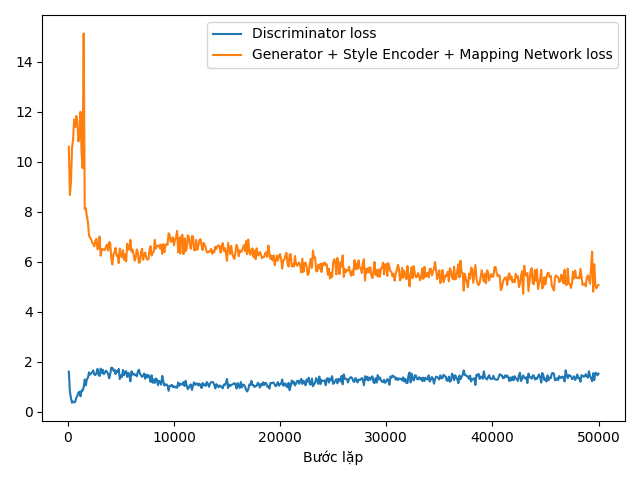
\includegraphics[width=\linewidth]{figure40.png}
    \caption{Giá trị hàm mục tiêu của các mạng thành phần qua thời gian.}
\end{figure}

Khác với quá trình học máy có giám sát, giá trị của hàm mục tiêu không nói lên nhiều về trạng thái hội tụ của mô hình. Dễ thấy từ đồ thị ở trên, hàm mục tiêu hầu như không thay đổi kể từ khoảng 15 nghìn bước lặp, song chất lượng ảnh đầu ra ở các bước lặp vẫn có sự khác biệt đáng kể. Để đánh giá chất lượng của mô hình, ta cần sử dụng một hàm đo hiệu quả hơn, so sánh được không gian xác suất giữa dữ liệu thật và dữ liệu giả sinh ra bởi generator.

Như đã chỉ ra trong mục \ref{convolutional-layer}, mạng CNN có khả năng nhận dạng và mã hóa các đặc điểm trên ảnh, và các lớp về sau có thể tổng hợp các thông tin phức tạp hơn từ kết quả của các lớp đầu tiên. Điều này khiến cho mạng CNN có khả năng mã hóa các đặc điểm nhận dạng hình học của dữ liệu ảnh, rất hữu ích cho nhiều ứng dụng sử dụng học máy. Đây cũng chính là tư tưởng cơ bản của độ đo Khoảng cách Nhận diện Frechet (Frechet Inception Distance hay FID) \cite{DBLP:journals/corr/HeuselRUNKH17}.

Độ đo FID so sánh hai tập hợp ảnh bất kì bằng cách sử dụng mạng Inception v3 - một trong những mạng học sâu đi đầu trong bài toán phân loại ảnh - để mã hóa các ảnh thuộc cả hai tập hợp. Sau khi loại bỏ lớp mạng cuối cùng chịu trách nhiệm phân loại, Inception v3 cho ra một vector 2048 chiều mã hóa đặc điểm của ảnh. FID tính khoảng cách giữa hai tập hợp ảnh bằng công thức:
$$ FID = ||\mu_1 - \mu_2||^2 + Tr(C_1 + C_2 - 2\sqrt{C_1 * C_2}) $$
trong đó:
\begin{itemize}
    \item $ \mu_1 $, $ \mu_2 $ và $ C_1 $, $ C_2 $ lần lượt là vector giá trị kì vọng và ma trận hiệp phương sai theo mỗi chiều của các vector mã hóa.
    \item $ ||x||^2 = \sum_{i=1}^{n} x_i^2 $.
    \item $ Tr(X) = \sum_{i=1}^{n} X_{i,i} $
\end{itemize}

Giá trị của độ đo FID càng thấp, hai tập hợp càng có đặc điểm giống nhau, với $ FID = 0 $ khi hai tập hợp hoàn toàn bằng nhau. Trên thực tế, ta không thể kì vọng $ FID = 0 $, thay vào đó ta lấy giá trị độ đo FID giữa hai tập ảnh thật ngẫu nhiên làm chuẩn để đánh giá chất lượng của tập ảnh sinh ra bởi mô hình GAN.

Để đánh giá chất lượng của mô hình, ta lấy ngẫu nhiên 100 ảnh từ mỗi chế độ màu. Với mỗi chế độ, ta sử dụng FID để so sánh tập hợp ảnh thật thuộc chế độ này với 3 tập hợp ảnh giả được chuyển đổi từ 3 chế độ còn lại, cùng với một bộ 100 ảnh thật thuộc cùng chế độ để lấy giá trị đối chiếu.

\begin{figure}[H]
    \centering
    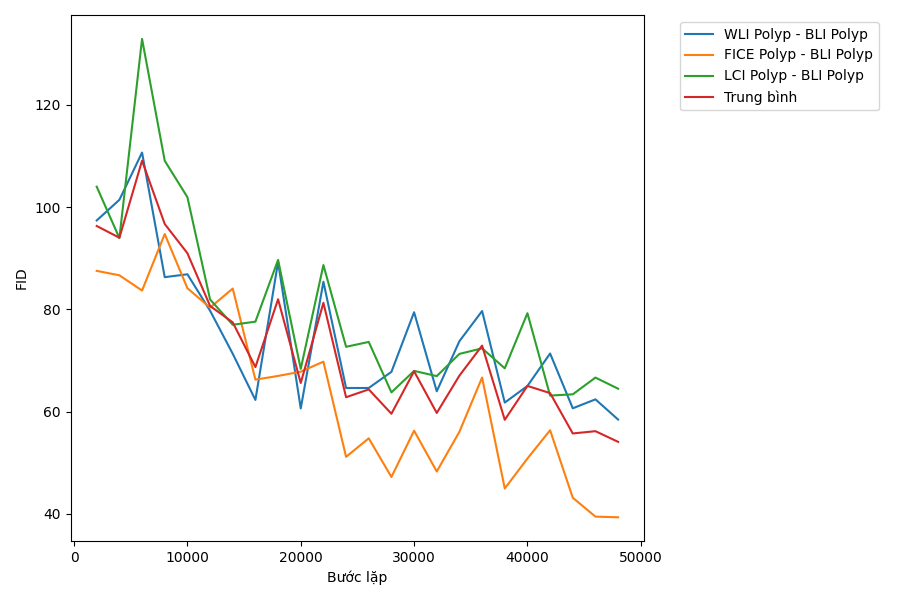
\includegraphics[width=\linewidth]{fid/FID_BLI.png}
    \caption{Giá trị độ đo FID qua các bước lặp khi chuyển đổi ảnh sang chế độ BLI.}
\end{figure}

\begin{figure}[H]
    \centering
    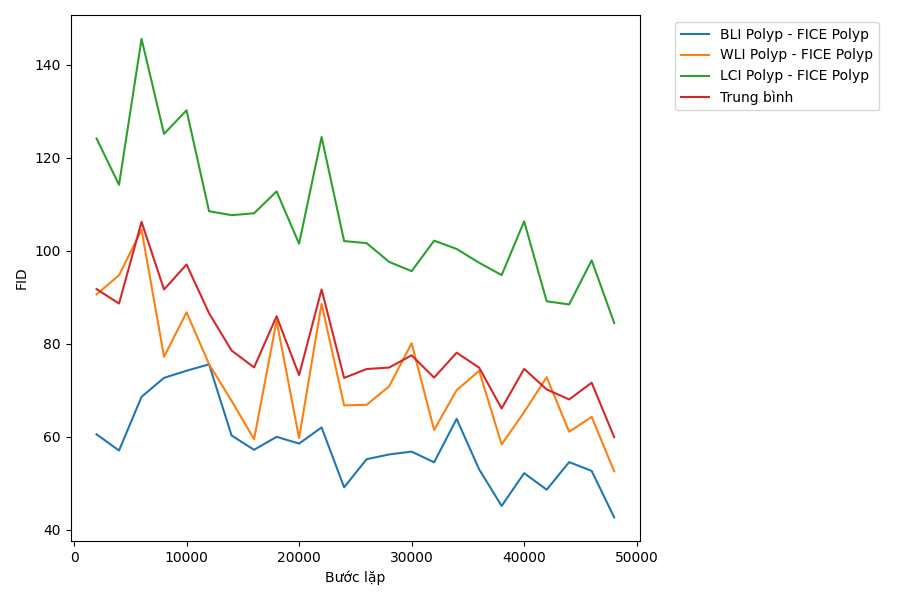
\includegraphics[width=\linewidth]{fid/FID_FICE.png}
    \caption{Giá trị độ đo FID qua các bước lặp khi chuyển đổi ảnh sang chế độ FICE.}
\end{figure}

\begin{figure}[H]
    \centering
    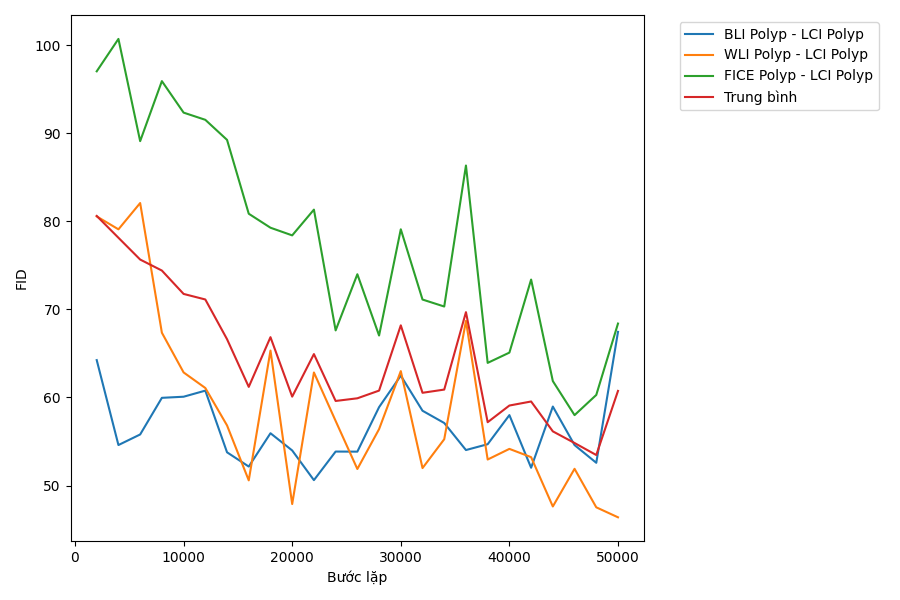
\includegraphics[width=\linewidth]{fid/FID_LCI.png}
    \caption{Giá trị độ đo FID qua các bước lặp khi chuyển đổi ảnh sang chế độ LCI.}
\end{figure}

\begin{figure}[H]
    \centering
    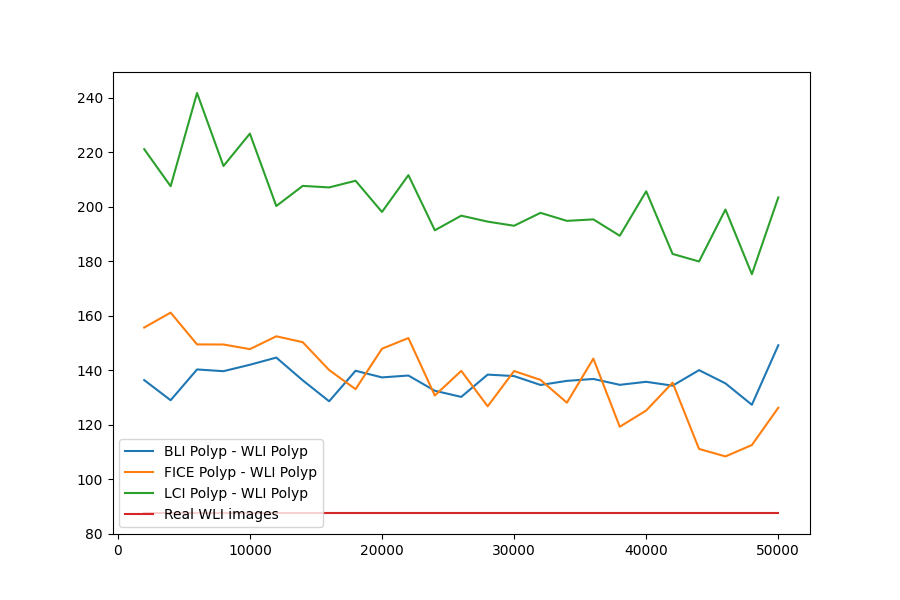
\includegraphics[width=\linewidth]{fid/FID_WLI.png}
    \caption{Giá trị độ đo FID qua các bước lặp khi chuyển đổi ảnh sang chế độ WLI.}
\end{figure}

Qua việc theo dõi độ đo FID, ta nhận thấy mô hình hoạt động tốt nhất theo cả hai hướng biến đổi đi và về khi làm việc với chế độ màu BLI và WLI, kém nhất với chế độ màu LCI. Điều này là có thể dự đoán được - như đã nói ở mục \ref{lci}, chế độ màu LCI có tính năng tô màu các khối u ung thư rất phức tạp, khó có thể tái tạo lại được trên mô hình. Ta sẽ làm rõ nhược điểm của ảnh LCI nhân tạo khi thực hiện đánh giá định tính.

Sau khi lấy trung bình giá trị FID trên tất cả các lớp ảnh, mô hình ở bước lặp thứ 48 nghìn được lựa chọn để sử dụng, vì giá trị độ đo FID của mô hình này là tốt nhất.

\subsection{Đánh giá định tính}

Quan sát kết quả chuyển đổi ảnh từ mỗi chế độ màu sang các chế độ còn lại, ta nhận thấy:
\begin{itemize}
    \item Mô hình làm tốt việc tái tạo lại màu sắc của các chế độ BLI, FICE và WLI. Riêng đối với LCI, ảnh bị pha màu vàng không tự nhiên - ảnh LCI thường có màu đỏ giống WLI, với các mạch máu nổi lên màu tím. Điều này giải thích lý do vì sao độ đo FID của lớp ảnh LCI là cao nhất trong cả 4 lớp.
    \item Vì kênh Y của ảnh được giữ cố định, bố cục của ảnh hoàn toàn được đảm bảo, song các đặc điểm về độ sáng và độ tương phản ảnh không được cải thiện nhiều khi chuyển sang các chế độ ảnh cao cấp. Độ tương phản chủ yếu được tăng cường bởi sự tương phản của các mảng màu trong ảnh.
    \item Vẫn còn hiện tượng nhiễu xuất hiện dưới dạng bóng tròn mờ trên ảnh, song không đáng kể.
\end{itemize}

\begin{table}[H]
    \centering
    \begin{tabular}{c | c | c | c | c}
        Chế độ gốc & BLI                                                                  & FICE                                                                  & LCI                                                                  & WLI                                                                  \\
        Ảnh gốc    & 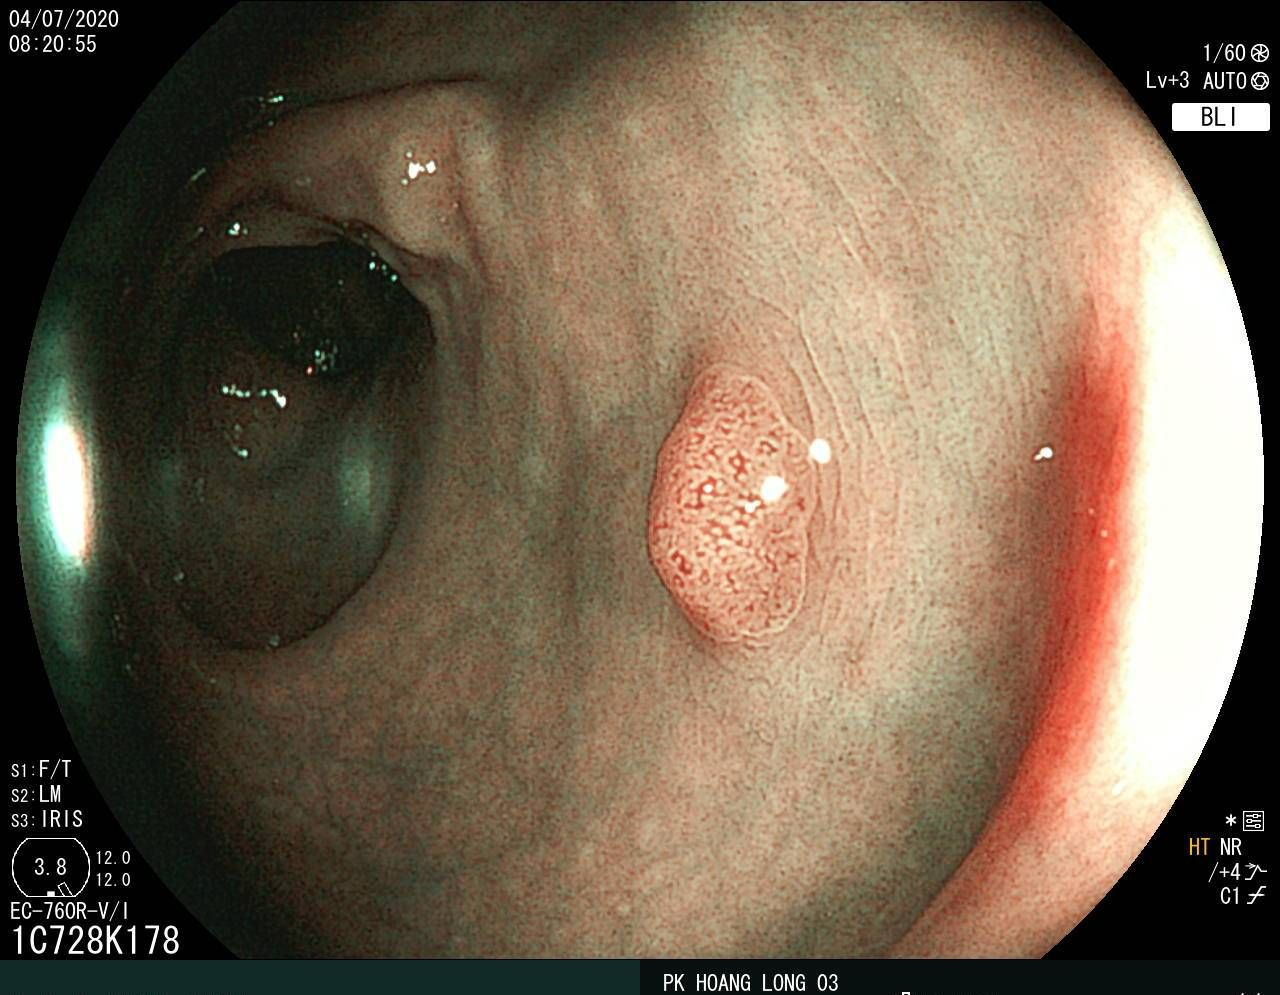
\includegraphics[width=0.185\textwidth]{transform/BLI_original.jpeg} & \includegraphics[width=0.185\textwidth]{transform/FICE_original.jpeg} & \includegraphics[width=0.185\textwidth]{transform/LCI_original.jpeg} & \includegraphics[width=0.185\textwidth]{transform/WLI_original.jpeg} \\
        \hline
        Sang BLI   &                                                                      & \includegraphics[width=0.185\textwidth]{transform/FICE2BLI.jpeg}      & \includegraphics[width=0.185\textwidth]{transform/LCI2BLI.jpeg}      & \includegraphics[width=0.185\textwidth]{transform/WLI2BLI.jpeg}      \\
        Sang FICE  & \includegraphics[width=0.185\textwidth]{transform/BLI2FICE.jpeg}     &                                                                       & \includegraphics[width=0.185\textwidth]{transform/LCI2FICE.jpeg}     & \includegraphics[width=0.185\textwidth]{transform/WLI2FICE.jpeg}     \\
        Sang LCI   & \includegraphics[width=0.185\textwidth]{transform/BLI2LCI.jpeg}      & \includegraphics[width=0.185\textwidth]{transform/FICE2LCI.jpeg}      &                                                                      & \includegraphics[width=0.185\textwidth]{transform/WLI2LCI.jpeg}      \\
        Sang WLI   & \includegraphics[width=0.185\textwidth]{transform/BLI2WLI.jpeg}      & \includegraphics[width=0.185\textwidth]{transform/FICE2WLI.jpeg}      & \includegraphics[width=0.185\textwidth]{transform/LCI2WLI.jpeg}      &                                                                      \\
    \end{tabular}
    \caption{Kết quả biến đổi giữa các chế độ màu với nhau.}
\end{table}

Nhìn chung, tuy không chuyển đổi được tất cả các tính năng của các chế độ màu cao cấp, mô hình StarGAN v2 có thể giúp tăng cường chất lượng và độ tương phản màu sắc của ảnh nội soi, giúp bác sĩ nội soi quan sát tốt hơn các đối tượng trong ảnh và đưa ra chẩn đoán chính xác hơn.

\begin{figure}[H]
    \centering
    \begin{subfigure}[H]{0.32\textwidth}
        \centering
        \includegraphics[width=\linewidth]{example/wli.png}
        \caption{Ảnh gốc WLI}
    \end{subfigure}
    \begin{subfigure}[H]{0.32\textwidth}
        \centering
        \includegraphics[width=\linewidth]{example/lci.jpeg}
        \caption{Ảnh chuyển đổi sang LCI}
    \end{subfigure}
    \begin{subfigure}[H]{0.32\textwidth}
        \centering
        \includegraphics[width=\linewidth]{example/lci_real.png}
        \caption{Ảnh thật LCI}
    \end{subfigure}
    \caption{Chuyển đổi ảnh ví dụ \ref{wli-lci} sang LCI. So với ảnh gốc, các đối tượng trong ảnh chuyển đổi tương phản rõ ràng hơn. Tuy nhiên khi so sánh với ảnh thật, ảnh chuyển đổi rọi sáng kém hơn ở phía xa và không làm nổi vùng tổn thương nhiều.}
\end{figure}

\chapter{Ứng dụng thực tế - áp dụng vào hệ thống Polyp-Labeler}
\label{application-polyp-labeler}

\chapter{Kết luận và hướng phát triển}

\newpage

\bibliography{pericles_1542486368.bib,5109748.bib,10613481.bib,15578301.bib,S0016510708028903.bib,S1590865809001960.bib,S0016508507007950.bib,20628363.bib,24373002.bib,30291440.bib,29539651.bib,26770267.bib,31700545.bib,srivastava14a.bib,citation339446790.bib,cs230.bib,NIPS-2014-generative-adversarial-nets-Bibtex.bib,duchi2011adaptive.bib,S0893608098001166.bib,kingma2017adam.bib,pix2pix2017.bib,CycleGAN2017.bib,cyclegan.bib,DBLP.bib,starganv2.bib,s0038401113808.bib,26668791.bib,choi2020stargan.bib,he2015deep.bib,batchnorm.bib,batchnorm_styletransfer.bib,instancenorm.bib,which_training.bib,fid.bib}

\end{document}
